%\documentclass[conference]{IEEEtran}
\documentclass[10pt, conference, letterpaper]{IEEEtran}


\usepackage{enumitem}

% *** CITATION PACKAGES ***
\usepackage{cite}
% *** GRAPHICS RELATED PACKAGES ***
\usepackage{graphicx}
\usepackage{caption}
\usepackage{subcaption}
\usepackage{refstyle}
% *** MATH PACKAGES ***
\usepackage[cmex10]{amsmath}
\DeclareMathOperator*{\argmin}{\arg\!\min}
% *** SPECIALIZED LIST PACKAGES ***
\usepackage{algorithmic}
% *** ALIGNMENT PACKAGES ***
\usepackage{array}
%\usepackage[font=footnotesize]{subfig}
\usepackage{url}
\usepackage{amsbsy}
\usepackage{fontenc}
\usepackage[utf8]{inputenc}
\usepackage{mathtools}
\usepackage{tabularx}
\usepackage{tabu}
\usepackage{float}
\usepackage{gensymb}
\usepackage{multirow}
\usepackage{siunitx}
\usepackage{bbold}
%\usepackage{algorithm}
\usepackage{algorithmic}
\usepackage{psfrag}
\usepackage{pgfplots}
\usepackage{xcolor}
\newcommand\note[1]{\textcolor{red}{#1}}
\usepackage{comment}
\usepackage{wrapfig}
%\usepackage{nopageno} %% clear page number%%%
\usepackage[utf8]{inputenc}
\usepackage{amsmath,amssymb}
\usepackage{makecell}
\usepackage{booktabs}
\usepackage{bm}
\usepackage{enumitem}
\usepackage{dblfloatfix}    % To enable figures at the bottom of page
%\usepackage[skip=5pt, format=plain, font=it]{caption}
%\usepackage{parskip}
\usepackage[ruled,vlined]{algorithm2e}
%\setlength{\abovedisplayskip}{1pt}
%\setlength{\belowdisplayskip}{1pt}
\usepackage{mathtools,nccmath}

%\usepackage{titling}
%\setlength{\droptitle}{-10pt}




\SetKwInput{KwInput}{Input}                
\SetKwInput{KwOutput}{Output}              
\usepackage{flushend}

%\setlength{\aboverulesep}{0pt}
%\setlength{\belowrulesep}{0pt}
\newcommand{\Rho}{\mathrm{P}}

%\DeclareMathSizes{9}{9}{5}{5} % This makes 9pt maths when the surrounding body text is (nominal) 10pt.

%\setlength{\textfloatsep}{0.1cm}

%\newcommand{\abbrev}{\texttt{LOCI}}

%% This is to add watermark
%\usepackage{draftwatermark}
%\SetWatermarkText{Draft}
%\SetWatermarkScale{1}
\newcommand{\navid}[1]{{\color{teal}{\bf #1}}}
\newcommand{\wenjun}[1]{{\color{blue}{\bf #1}}}
\newcommand{\ahmed}[1]{{\color{green}{\bf #1}}}
%%%%%%%%%%%%%%%%%%%%%%%%%%%%%%%%%%%%%%%%%%%%%%%%%%%%%%%%%%%%%%%%%%%%%%%%%
%%%%%%%%%%%%%%%%%%%%%%%%%%%%%%%%%%%%%%%%%%%%%%%%%%%%%%%%%%%%%%%%%%%%%%%%%
%%%%%%%%%%%%%%%%%%%%%%%%%%%%%%%%%%%%%%%%%%%%%%%%%%%%%%%%%%%%%%%%%%%%%%%%%
\newsavebox{\ieeealgbox}
\newenvironment{boxedalgorithmic}
  {\begin{lrbox}{\ieeealgbox}
   \begin{minipage}{\dimexpr\columnwidth-2\fboxsep-2\fboxrule}
   \begin{algorithmic}}
  {\end{algorithmic}
   \end{minipage}
   \end{lrbox}\noindent\fbox{\usebox{\ieeealgbox}}}
\newcolumntype{M}[1]{>{\arraybackslash}m{#1}}
\newcolumntype{N}{@{}m{0pt}@{}}
%%%%%%%%%%%%%%%%%%%%%%%%%%%%%%%%%%%%%%%%%%%%%%%%%%%%%%%%%%%%%%%%%%%%%%%%%
%%%%%%%%%%%%%%%%%%%%%%%%%%%%%%%%%%%%%%%%%%%%%%%%%%%%%%%%%%%%%%%%%%%%%%%%%
%%%%%%%%%%%%%%%%%%%%%%%%%%%%%%%%%%%%%%%%%%%%%%%%%%%%%%%%%%%%%%%%%%%%%%%%%
%\usepackage[utf8]{inputenc}
%\usepackage[english]{babel}
%\usepackage{amsthm}
\newtheorem{theorem}{Theorem}[section]
\newtheorem{corollary}{Corollary}[theorem]
\newtheorem{lemma}{Lemma}
%\newtheorem{proof}{Proof}[theorem]
\newtheorem{proof}{Proof}
\usepackage{proof}

%\IEEEoverridecommandlockouts
\setlength{\abovedisplayskip}{2pt}
\setlength{\belowdisplayskip}{2pt}

\begin{document}

%\title{Domain Knowledge Guided Neural Network\\ for Wireless Channel Estimation\\}
%\title{Bridging the Gap between Data Driven and Model Based Approach for Wireless Communication}
%\title{Learning the Receiver for Terahertz Communication}

%\title{Neural Network based Receiver\\ for Terahertz Communication}
\title{%\texttt{LOCAL}: \underline{L}ow \underline{O}verhead \underline{L}earning based \underline{C}ollabor\underline{A}tive Interference Cancellation for Radio Astronomy\\
Digital-Twin assisted Network Energy Optimization during Low Traffic Hours}
\begin{comment}
\author{
\IEEEauthorblockN{Shuvam Chakraborty$^{\dagger}$, Ahmed Bedewy$^*$, Wenjun Li$^*$, Navid Abedini$^*$}
\IEEEauthorblockA{$^\dagger$ Department of Electrical \& Computer Engineering, University at Albany, SUNY, USA  - e-mail: schakraborty@albany.edu}
$^*$Qualcomm Technologies Inc. - e-mail: \{ahmebede, wenjunl, navida\}@qti.qualcomm.com
\vspace{0mm}

%\thanks{}
}
\end{comment}

\author{
\IEEEauthorblockN{Shuvam Chakraborty, Ahmed Bedewy, Wenjun Li, Navid Abedini}
\IEEEauthorblockA{
$^*$Qualcomm Technologies Inc. - e-mail: \{shuvchak, ahmebede, wenjunl, navida\}@qti.qualcomm.com}
\vspace{0mm}

%\thanks{}
}
\begin{comment}
\author{\IEEEauthorblockN{Shuvam Chakraborty}
\IEEEauthorblockA{
Department of Electrical \& Computer Engineering \\
University at Albany, SUNY, Albany, NY 12222 USA\\
\{schakraborty\}@albany.edu}
\navid{please put all the names together!}
\and
\IEEEauthorblockN{Ahmed Bedewy, Wenjun Li and Navid Abedini}
\IEEEauthorblockA{
Qualcomm Technologies, Inc.\\
%California Institute of Technology, CA,  USA\\
\{ahmebede, wenjunl, navida\}@qti.qualcomm.com}
%\vspace{-25ex}
}
\end{comment}
%\thanks{Shuvam Chakraborty and Hesham Mohammed are co-first authors.}
%% This is taken from IEEE http://ieeeauthorcenter.ieee.org/wp-content/uploads/IEEE_Style_Manual.pdf 

%\vspace*{-20pt}

\maketitle
%\thispagestyle{empty}
\pagestyle{empty}
%\pagestyle{plain}
%\raggedbottom

\begin{abstract}  
Test time scaling is currently one of the most active research areas that shows promise after training time scaling has reached its limits.
Deep-thinking (DT) models are a class of recurrent models that can perform easy-to-hard generalization by assigning more compute to harder test samples.
However, due to their inability to determine the complexity of a test sample, DT models have to use a large amount of computation for both easy and hard test samples.
Excessive test time computation is wasteful and can cause the ``overthinking'' problem where more test time computation leads to worse results.
In this paper, we introduce a test time training method for determining the optimal amount of computation needed for each sample during test time.
We also propose Conv-LiGRU, a novel recurrent architecture for efficient and robust visual reasoning. 
Extensive experiments demonstrate that Conv-LiGRU is more stable than DT, effectively mitigates the ``overthinking'' phenomenon, and achieves superior accuracy.
\end{abstract}  
\section{Introduction}


\begin{figure}[t]
\centering
\includegraphics[width=0.6\columnwidth]{figures/evaluation_desiderata_V5.pdf}
\vspace{-0.5cm}
\caption{\systemName is a platform for conducting realistic evaluations of code LLMs, collecting human preferences of coding models with real users, real tasks, and in realistic environments, aimed at addressing the limitations of existing evaluations.
}
\label{fig:motivation}
\end{figure}

\begin{figure*}[t]
\centering
\includegraphics[width=\textwidth]{figures/system_design_v2.png}
\caption{We introduce \systemName, a VSCode extension to collect human preferences of code directly in a developer's IDE. \systemName enables developers to use code completions from various models. The system comprises a) the interface in the user's IDE which presents paired completions to users (left), b) a sampling strategy that picks model pairs to reduce latency (right, top), and c) a prompting scheme that allows diverse LLMs to perform code completions with high fidelity.
Users can select between the top completion (green box) using \texttt{tab} or the bottom completion (blue box) using \texttt{shift+tab}.}
\label{fig:overview}
\end{figure*}

As model capabilities improve, large language models (LLMs) are increasingly integrated into user environments and workflows.
For example, software developers code with AI in integrated developer environments (IDEs)~\citep{peng2023impact}, doctors rely on notes generated through ambient listening~\citep{oberst2024science}, and lawyers consider case evidence identified by electronic discovery systems~\citep{yang2024beyond}.
Increasing deployment of models in productivity tools demands evaluation that more closely reflects real-world circumstances~\citep{hutchinson2022evaluation, saxon2024benchmarks, kapoor2024ai}.
While newer benchmarks and live platforms incorporate human feedback to capture real-world usage, they almost exclusively focus on evaluating LLMs in chat conversations~\citep{zheng2023judging,dubois2023alpacafarm,chiang2024chatbot, kirk2024the}.
Model evaluation must move beyond chat-based interactions and into specialized user environments.



 

In this work, we focus on evaluating LLM-based coding assistants. 
Despite the popularity of these tools---millions of developers use Github Copilot~\citep{Copilot}---existing
evaluations of the coding capabilities of new models exhibit multiple limitations (Figure~\ref{fig:motivation}, bottom).
Traditional ML benchmarks evaluate LLM capabilities by measuring how well a model can complete static, interview-style coding tasks~\citep{chen2021evaluating,austin2021program,jain2024livecodebench, white2024livebench} and lack \emph{real users}. 
User studies recruit real users to evaluate the effectiveness of LLMs as coding assistants, but are often limited to simple programming tasks as opposed to \emph{real tasks}~\citep{vaithilingam2022expectation,ross2023programmer, mozannar2024realhumaneval}.
Recent efforts to collect human feedback such as Chatbot Arena~\citep{chiang2024chatbot} are still removed from a \emph{realistic environment}, resulting in users and data that deviate from typical software development processes.
We introduce \systemName to address these limitations (Figure~\ref{fig:motivation}, top), and we describe our three main contributions below.


\textbf{We deploy \systemName in-the-wild to collect human preferences on code.} 
\systemName is a Visual Studio Code extension, collecting preferences directly in a developer's IDE within their actual workflow (Figure~\ref{fig:overview}).
\systemName provides developers with code completions, akin to the type of support provided by Github Copilot~\citep{Copilot}. 
Over the past 3 months, \systemName has served over~\completions suggestions from 10 state-of-the-art LLMs, 
gathering \sampleCount~votes from \userCount~users.
To collect user preferences,
\systemName presents a novel interface that shows users paired code completions from two different LLMs, which are determined based on a sampling strategy that aims to 
mitigate latency while preserving coverage across model comparisons.
Additionally, we devise a prompting scheme that allows a diverse set of models to perform code completions with high fidelity.
See Section~\ref{sec:system} and Section~\ref{sec:deployment} for details about system design and deployment respectively.



\textbf{We construct a leaderboard of user preferences and find notable differences from existing static benchmarks and human preference leaderboards.}
In general, we observe that smaller models seem to overperform in static benchmarks compared to our leaderboard, while performance among larger models is mixed (Section~\ref{sec:leaderboard_calculation}).
We attribute these differences to the fact that \systemName is exposed to users and tasks that differ drastically from code evaluations in the past. 
Our data spans 103 programming languages and 24 natural languages as well as a variety of real-world applications and code structures, while static benchmarks tend to focus on a specific programming and natural language and task (e.g. coding competition problems).
Additionally, while all of \systemName interactions contain code contexts and the majority involve infilling tasks, a much smaller fraction of Chatbot Arena's coding tasks contain code context, with infilling tasks appearing even more rarely. 
We analyze our data in depth in Section~\ref{subsec:comparison}.



\textbf{We derive new insights into user preferences of code by analyzing \systemName's diverse and distinct data distribution.}
We compare user preferences across different stratifications of input data (e.g., common versus rare languages) and observe which affect observed preferences most (Section~\ref{sec:analysis}).
For example, while user preferences stay relatively consistent across various programming languages, they differ drastically between different task categories (e.g. frontend/backend versus algorithm design).
We also observe variations in user preference due to different features related to code structure 
(e.g., context length and completion patterns).
We open-source \systemName and release a curated subset of code contexts.
Altogether, our results highlight the necessity of model evaluation in realistic and domain-specific settings.





\putsec{related}{Related Work}

\noindent \textbf{Efficient Radiance Field Rendering.}
%
The introduction of Neural Radiance Fields (NeRF)~\cite{mil:sri20} has
generated significant interest in efficient 3D scene representation and
rendering for radiance fields.
%
Over the past years, there has been a large amount of research aimed at
accelerating NeRFs through algorithmic or software
optimizations~\cite{mul:eva22,fri:yu22,che:fun23,sun:sun22}, and the
development of hardware
accelerators~\cite{lee:cho23,li:li23,son:wen23,mub:kan23,fen:liu24}.
%
The state-of-the-art method, 3D Gaussian splatting~\cite{ker:kop23}, has
further fueled interest in accelerating radiance field
rendering~\cite{rad:ste24,lee:lee24,nie:stu24,lee:rho24,ham:mel24} as it
employs rasterization primitives that can be rendered much faster than NeRFs.
%
However, previous research focused on software graphics rendering on
programmable cores or building dedicated hardware accelerators. In contrast,
\name{} investigates the potential of efficient radiance field rendering while
utilizing fixed-function units in graphics hardware.
%
To our knowledge, this is the first work that assesses the performance
implications of rendering Gaussian-based radiance fields on the hardware
graphics pipeline with software and hardware optimizations.

%%%%%%%%%%%%%%%%%%%%%%%%%%%%%%%%%%%%%%%%%%%%%%%%%%%%%%%%%%%%%%%%%%%%%%%%%%
\myparagraph{Enhancing Graphics Rendering Hardware.}
%
The performance advantage of executing graphics rendering on either
programmable shader cores or fixed-function units varies depending on the
rendering methods and hardware designs.
%
Previous studies have explored the performance implication of graphics hardware
design by developing simulation infrastructures for graphics
workloads~\cite{bar:gon06,gub:aam19,tin:sax23,arn:par13}.
%
Additionally, several studies have aimed to improve the performance of
special-purpose hardware such as ray tracing units in graphics
hardware~\cite{cho:now23,liu:cha21} and proposed hardware accelerators for
graphics applications~\cite{lu:hua17,ram:gri09}.
%
In contrast to these works, which primarily evaluate traditional graphics
workloads, our work focuses on improving the performance of volume rendering
workloads, such as Gaussian splatting, which require blending a huge number of
fragments per pixel.

%%%%%%%%%%%%%%%%%%%%%%%%%%%%%%%%%%%%%%%%%%%%%%%%%%%%%%%%%%%%%%%%%%%%%%%%%%
%
In the context of multi-sample anti-aliasing, prior work proposed reducing the
amount of redundant shading by merging fragments from adjacent triangles in a
mesh at the quad granularity~\cite{fat:bou10}.
%
While both our work and quad-fragment merging (QFM)~\cite{fat:bou10} aim to
reduce operations by merging quads, our proposed technique differs from QFM in
many aspects.
%
Our method aims to blend \emph{overlapping primitives} along the depth
direction and applies to quads from any primitive. In contrast, QFM merges quad
fragments from small (e.g., pixel-sized) triangles that \emph{share} an edge
(i.e., \emph{connected}, \emph{non-overlapping} triangles).
%
As such, QFM is not applicable to the scenes consisting of a number of
unconnected transparent triangles, such as those in 3D Gaussian splatting.
%
In addition, our method computes the \emph{exact} color for each pixel by
offloading blending operations from ROPs to shader units, whereas QFM
\emph{approximates} pixel colors by using the color from one triangle when
multiple triangles are merged into a single quad.


\section{Problem Formulation} \label{sec:probdef}

This section formally defines the problem of restoring a given pruned network with only using its original pretrained CNN in a way free of data and fine-tuning.



% Unlike many existing works utilize data for identifying unimportant filters as well as fine-tuning to this end, we cannot evaluate the filter importance by data-dependent values like activation maps (\textit{a.k.a.} channels) as our focus in this paper is not to use any training data. Thus, in our problem setting, we can only exploit the values of filters in the original network, and thereby have to make some changes in the remaining filters of the pruned network so that the network can return the output not too much different from the original one.

% No matter how much we carefully select unimportant filters to be pruned, some kinds of retraining process appears inevitable as done by the most existing works to this end. However, since our focus in this paper is not to use any training data, we cannot evaluate the importance of filters by data-dependent values like activation maps (\textit{a.k.a.} channels). 

% To this end, they not only use a careful criterion (\textit{e.g.}, L1-norm), but also fine-tune the network using the original data.
% Most of filter pruning methods try to select filters to be pruned prudently so that pruned network's output be similar to the original network's. To this end, they prune the unimportant filters and then fine-tune the pruned network with using the train data. 

% How can we restore the the pruned networks without any data? In other words, it implies that we cannot use any data-driven values(i.e., activation maps) and we can only exploit the values of original filters. In that case, the only thing we can do maybe changing the weights of remained filters appropriately not to amplify the difference between pruned and unpruned network's outputs through the information of original filters.

\begin{figure*}[t]
	\centering
    \subfigure[\label{fig:matrix:a}Pruning matrix]{\hspace{6mm}\includegraphics[width=0.35\columnwidth]{./figure/LBYL_figure_2_1.pdf}\hspace{6mm}} 
    \subfigure[\label{fig:matrix:b}Delivery matrix for LBYL]{\hspace{6mm}\includegraphics[width=0.35\columnwidth]{./figure/LBYL_figure_2_2.pdf}\hspace{6mm}}
    \subfigure[\label{fig:matrix:c}Delivery matrix for one-to-one]{\hspace{9mm}\includegraphics[width=0.35\columnwidth]{./figure/LBYL_figure_2_3.pdf}\hspace{9mm}} 
    \caption{Comparison between pruning matrix and delivery matrix, where the $4$-th and $6$-th filters are being pruned among $6$ original filters}
	\label{fig:matrix}
	\vspace{-2mm}
\end{figure*}



\subsection{Filter Pruning in a CNN}
Consider a given CNN to be pruned with $L$ layers, where each $\ell$-th layer starts with a convolution operation on its input channels, which are the output of the previous $(\ell-1)$-th layer $\mathbf{A}^{(\ell-1)}$, with the group of convolution filters $\mathbf{W}^{{(\ell)}}$ and thereby obtain the set of \textit{feature maps} $\mathbf{Z}^{(\ell)}$ as follows:
\begin{equation}
\boldsymbol{\mathbf{Z}}^{(\ell)} = {\mathbf{A}^{(\ell-1)} \circledast {\mathbf{W}}^{(\ell)}},
\nonumber
\end{equation}
where $\circledast$ represents the convolution operation. Then, this convolution process is normally followed by a batch normalization (BN) process and an activation function such as ReLU, and the $\ell$-th layer finally outputs an \textit{activation map} $\mathbf{A}^{(\ell)}$ to be sent to the $(\ell+1)$-th layer through this sequence of procedures as:
\begin{equation}
\mathbf{A}^{(\ell)} = \F(\N(\mathbf{Z}^{(\ell)})),
\nonumber
\end{equation}
where $\F(\cdot)$ is an activation function and $\N(\cdot)$ is a BN procedure.

Note that all of $\mathbf{W}^{(\ell)}$, $\mathbf{Z}^{(\ell)}$, and $\mathbf{A}^{(\ell)}$ are tensors such that: $\mathbf{W}^{(\ell)} \in \mathbb{R}^{m \times n \times k \times k}$ and $\mathbf{Z}^{(\ell)},\mathbf{A}^{(\ell)} \in \mathbb{R}^{m \times w \times h}$, where (1) $m$ is the number of filters, which also equals the number of output activation maps, (2) $n$ is the number of input activation maps resulting from the $(\ell-1)$-th layer, (3) $k \times k$ is the size of each filter, and (4) $w \times h$ is the size of each output channel for the $\ell$-th layer.

\smalltitle{Filter pruning as n-mode product}
When filter pruning is performed at the $\ell$-th layer, all three tensors above are consequently modified to their \textit{damaged} versions, namely $\mathbf{\Tilde{W}}^{(\ell)}$, $\mathbf{\Tilde{Z}}^{(\ell)}$, and $\mathbf{\Tilde{A}}^{(\ell)}$, respectively, in a way that: $\mathbf{\Tilde{W}}^{(\ell)} \in \mathbb{R}^{t \times n \times k \times k}$ and $\mathbf{\Tilde{Z}}^{(\ell)},\mathbf{\Tilde{A}}^{(\ell)} \in \mathbb{R}^{t \times w \times h}$, where $t$ is the number of remaining filters after pruning and therefore $t < m$. Mathematically, the tensor of remaining filters, \textit{i.e.}, $\mathbf{\Tilde{W}}^{(\ell)}$, is obtained by the \textit{$1$-mode product} \cite{DBLP:journals/siamrev/KoldaB09} of the tensor of the original filters $\mathbf{W}^{(\ell)}$ with a \textit{pruning matrix} $\boldsymbol{\S} \in \mathbb{R}^{m \times t}$ (see Figure \ref{fig:matrix:a})
as follows:
\begin{eqnarray}\begin{split}\label{eq:pruning}
\mathbf{\Tilde{W}}^{(\ell)} = {\mathbf{W}}^{(\ell)} \times_{1} {\boldsymbol{\S}}^{T},\text{where }\boldsymbol{\S}_{i,k} = 
  \begin{cases} 
   1~ \text{if } i = i'_k \\
   0~ \text{otherwise}
  \end{cases} \\
  \text{s.t. } i, i'_k \in [1, m] 
  \text{ and } k \in [1, t].
  \end{split}
\end{eqnarray}
  
By Eq. (\ref{eq:pruning}), each $i'_k$-th filter is not pruned and the other $(m-t)$ filters are completely removed from $\mathbf{W}^{(\ell)}$ to be $\mathbf{\Tilde{W}}^{(\ell)}$.

This reduction at the $\ell$-th layer causes another reduction for each filter of the $(\ell+1)$-th layer so that $\mathbf{W}^{(\ell+1)}$ is now modified to $\mathbf{\Tilde{W}}^{(\ell+1)} \in \mathbb{R}^{m' \times t \times k' \times k'}$, where $m'$ is the number of filters of size $k' \times k'$ in the $(\ell+1)$-th layer. Due to this series of information losses, the resulting feature map (\textit{i.e.}, $\mathbf{Z}^{(\ell+1)}$) would severely be damaged to be $\mathbf{\Tilde{Z}}^{(\ell+1)}$ as shown below:
\begin{equation}
{\mathbf{\Tilde{Z}}}^{{(\ell+1)}} = \mathbf{\Tilde{A}}^{(\ell)} \circledast {\mathbf{\Tilde{W}}}^{(\ell+1)}~~~\not\approx~~~\mathbf{Z}^{(\ell+1)}
\label{eq:eq}\nonumber
\end{equation}
The shape of $\mathbf{\Tilde{Z}}^{(\ell+1)}$ remains the same unless we also prune filters for the $(\ell+1)$-th layer. If we do so as well, the loss of information will be accumulated and further propagated to the next layers. Note that $\mathbf{\Tilde{W}}^{(\ell+1)}$ can also be represented by the \textit{$2$-mode product} \cite{DBLP:journals/siamrev/KoldaB09} of $\mathbf{W}^{(\ell+1)}$ with the transpose of the same matrix $\boldsymbol{\S}$ as:
\begin{equation} \label{eq:pruning2}
\mathbf{\Tilde{W}}^{(\ell+1)} = {\mathbf{W}}^{(\ell+1)} \times_{2} {\boldsymbol{\S}^T}
\end{equation}




\subsection{Problem of Restoring a Pruned Network without Data and Fine-Tuning}
As mentioned earlier, our goal is to restore a pruned and thus damaged CNN without using any data and re-training process, which implies the following two facts. First, we have to use a pruning criterion exploiting only the values of filters themselves such as L1-norm. In this sense, this paper does not focus on proposing a sophisticated pruning criterion but intends to recover a network somehow pruned by such a simple criterion. Secondly, since we cannot make appropriate changes in the remaining filters by fine-tuning, we should make the best use of the original network and identify how the information carried by a pruned filter can be delivered to the remaining filters.

% For brevity, we formulate our problem here with respect to a specific layer, say $\ell$, and then it can trivially be generalized for the entire network. 
\smalltitle{Delivery matrix}
In order to represent the information to be delivered to the preserved filters, let us first think of what the pruning matrix $\boldsymbol{\S}$ means. As defined in Eq. (\ref{eq:pruning}) and shown in Figure \ref{fig:matrix:a}, each row is either a zero vector (for filters being pruned) or a one-hot vector (for remaining filters), which is intended only to remove filters without delivering any information. Intuitively, we can transform this pruning matrix into a \textit{delivery matrix} that carries information for filters being pruned by replacing some meaningful values with some of the zero values therein. Once we find such an \textit{ideal} $\boldsymbol{\S^*}$, we can plug it into $\boldsymbol{\S}$ of Eq. (\ref{eq:pruning2}) to deliver missing information propagated from the $\ell$-th layer to the filters at the $(\ell+1)$-th layer, which will hopefully generate an approximation $\mathbf{\hat{Z}}^{(\ell+1)}$ close to the original feature map as follows:
\begin{equation} \label{eq:fmap_approx}
{\mathbf{\hat{Z}}}^{{(\ell+1)}} = {\mathbf{\Tilde{A}}^{(\ell)} \circledast ({\mathbf{W}}^{(\ell+1)} \times_{2} {\boldsymbol{\S^*}^T})}
~~~\approx~~~\mathbf{Z}^{(\ell+1)}
\end{equation}
Thus, using the delivery matrix $\boldsymbol{\mathcal{S^*}}$, the information loss caused by pruning at each layer is recovered at the feature map of the next layer.

\smalltitle{Problem statement}
Given a pretrained CNN, our problem aims to find the best delivery matrix $\boldsymbol{\mathcal{S^*}}$ for each layer without any data and training process such that the following \textit{reconstruction error} is minimized:
\begin{equation}
\sum\limits_{i = 1}^{m'}\|{{\mathbf{Z}}_{i}^{{(\ell+1)}}-{\hat{\mathbf{Z}}}_{i}^{{(\ell+1)}}}\|_1,
\label{eq:goal}
\end{equation}
where ${\mathbf{Z}}_i^{{(\ell+1)}}$ and ${\hat{\mathbf{Z}}}_i^{{(\ell+1)}}$ indicate the $i$-th original feature map and its corresponding approximation, respectively, out of $m'$ filters in the $(\ell+1)$-th layer. Note that what is challenging here is that we cannot obtain the activation maps in $\mathbf{A}^{(\ell)}$ and $\mathbf{\Tilde{A}}^{(\ell)}$ without data as they are data-dependent values.

% = \sum\limits_{i = 1}^{m'}\|{{\mathbf{Z}}_{i}^{{(\ell+1)}}-{\mathbf{\Tilde{A}}^{(\ell)} \circledast ({\mathbf{W}}^{(\ell+1)} \times_{2} {\boldsymbol{\mathcal{S^*}^T}})}}\|_{1}


% Our goal is finding the approximation matrix $\boldsymbol{\mathcal{S}}$ to minimize the reconstruction error between the pruned model and the original model without any data, and effectively deliver missing information for pruned filters using this approximation matrix


% $\testit{s}$,which can be represented as below.

% \begin{equation}
% \boldsymbol{\mathcal{S}} =  \underset{{\boldsymbol{\mathcal{S}}}}{\mathrm{argmin}} \sum\limits_{{i} = 1}^{m_{\ell+1}} \|{{\mathbf{Z}}_{i,:,:}^{{(\ell+1)}}-{\hat{\mathbf{Z}}}_{i,:,:}^{{(\ell+1)}}}\|_{1} 
% \label{eq:eq1}
% \end{equation}



% Let us first recall that the ultimate goal of network pruning is to make the output of a pruned network as close as possible to that of its original network. Unlike many existing pruning methods, our focus is not to use any training data at all for the entire pruning and recovery process, and this implies the following two facts. First, we cannot evaluate the filter importance by data-dependent values like activation values or gradients, but have to use a pruning criterion exploiting only the values of filters themselves such as L1-norm. Furthermore, instead of fine-tuning with data, the only thing we can do for the pruned network is to make appropriate changes in the remaining filters by identifying some relationships between pruned filters and the other preserved ones without any support from data. Based on this intuition, this section mathematically and generally defines the problem of restoring a pruned neural network in a manner free of data and fine-tuning.


% Thus, we make approximation matrix $\testit{s}$ $\in$ $\mathbb{R}^{m_{\ell} \times t_{\ell}}$ with relationship between the pruned filter and preserved filters in $\ell$-th layer and then apply it to the original filters in $(\ell+1)$-th layer to compensate for pruned feature maps $\boldsymbol{\hat{\mathbf{Z}}}^{{(\ell+1)}}$ as shown below.
% (\textit{i.e.}, Let $\hat{\mathbf{W}}^{(\ell+1)}$ be ${\mathbf{W}}^{(\ell+1)}$ $\times_2$ ${{\textit{s}}} $, where $\times_2$ is 2-mode matrix product) 

% \begin{equation}
% \mathbf{Z}^{(\ell+1)} = {\mathbf{A}}^{(\ell)} \circledast {\mathbf{W}}^{(\ell+1)}
% \approx {\hat{\mathbf{A}}^{(\ell)} \circledast ({\mathbf{W}}^{(\ell+1)} \times_{2} {{s}}) = {\hat{\mathbf{Z}}}^{{(\ell+1)}}}
% \label{eq:eq}\nonumber
% \end{equation}




% For a Convolutional Neural Network (CNN) with $L$ layers, we denote $\mathcal{A}{^{(\ell-1)}}$ $\in$ $\mathbb{R}^{n_{\ell -1 } \times h_{\ell -1} \times w_{\ell -1}}$ is activation maps at $\ell-1$-th layer, where $n_{\ell -1}$, $h_{\ell -1}$ and $w_{\ell -1}$ are the number of channels, height and width in activation maps, respectively. and we denote $\mathbf{W}^{{(\ell )}}$ $\in$  $\mathbb{R}^{m_{\ell} \times n_{\ell -1}\times k \times k}$ is covolution filters in $\ell$-th layer,where $m_{\ell}$, $n_{\ell-1}$ and $k$ are the number of filters, number of channels and kernel size, respectively. Trough the convolution operation using activation map $\mathcal{A}{^{(\ell-1)}}$ and convolution filter $\mathbf{W}^{{(\ell)}}$ in $\ell$-th layer, the feature maps $\boldsymbol{\mathbf{Z}}^{{(\ell)}}$ $\in$ $\mathbb{R}^{m_{\ell} \times h_{\ell+1} \times w_{\ell+1}}$ is computed as shown as below.


% \begin{equation}
% \boldsymbol{\mathbf{Z}}^{(\ell)} = {\mathcal{A}^{(\ell-1)} \circledast {\mathbf{W}}^{(\ell)}}
% \label{eq:eq1}\nonumber
% \end{equation}
% where $\circledast$ is convolution operation.

% and the feature maps passed through the BN and ReLU layer are activation maps $\mathcal{A}{^{(\ell)}}$ $\in$ $\mathbb{R}^{m_{{\ell}} \times h_{\ell+1} \times w_{\ell+1}} $ in $\ell$-th layer as shown as below.

% \begin{equation}
% \mathcal{A}^{(\ell)} = \mathcal{F}(\mathbf{Z}^{(\ell)} \circledast {\mathbf{W}}^{(\ell)})
% \label{eq:eq2}\nonumber
% \end{equation}
% where $\mathcal{F}$ is the function that implement batch normalization and non-linear activation(\textit{e.g.}, ReLU).

% \smalltitle{Filter Pruning}
% If the filter pruning is performed in $\ell$-th layer, the shape of original filters $\mathbf{W}^{{(\ell)}}$ $\in$ $\mathbb{R}^{m_{\ell} \times n_{\ell-1}\times k \times k}$ is modified to ${\hat {\mathbf{W}}^{(\ell)}}$ $\in$ $\mathbb{R}^{t_{\ell} \times n_{\ell-1}\times k \times k}$, where $t_{\ell}$ $<$ $m_{\ell}$ by pruning criterion. Therefore, the pruned activation maps ${\hat {\mathcal{A}}}{^{({\ell+1})}}$ $\in$ $\mathbb{R}^{t_{{\ell}} \times h_{{\ell+2}} \times w_{{\ell+2}}}$ in (${\ell+1}$)-th layer is computed as below.

% \begin{equation}
% \mathbf{\hat{A}}^{(l+1)} = \mathcal{F}({\mathbf{A}^{(\ell)} \circledast {\mathbf{\hat{W}}}^{(\ell+1)}})
% \label{eq:eq3}\nonumber
% \end{equation}

% Moreover, corresponding channels of each filters in ($\ell +1$)-th layer are sequentially removed. As a result, shape of original filters $\mathbf{W}^{{(\ell+1)}}$ $\in$ $\mathbb{R}^{m_{\ell+1} \times m_{\ell}\times k \times k}$ in ($\ell+1$)-th layer is changed to  ${\hat {\mathbf{W}}^{(\ell+1)}}$ $\in$ $\mathbb{R}^{m_{\ell+1} \times t_{\ell}\times k \times k}$. Although feature maps ${\hat{\mathbf{Z}}}^{{(\ell+1)}}$ $\in$ $\mathbb{R}^{m_{\ell+1} \times h_{\ell+2} \times w_{\ell+2}}$ in ($\ell+1$)-th layer after pruning have same shape with original feature maps ${\mathbf{Z}}^{{(\ell+1)}}$ $\in$ $\mathbb{R}^{m_{\ell+1} \times h_{\ell+2} \times w_{\ell+2}}$, the pruned feature maps $\boldsymbol{\hat{\mathbf{Z}}}^{{(\ell+1)}}$ are damaged.
%\putsec{related}{Related Work}

\noindent \textbf{Efficient Radiance Field Rendering.}
%
The introduction of Neural Radiance Fields (NeRF)~\cite{mil:sri20} has
generated significant interest in efficient 3D scene representation and
rendering for radiance fields.
%
Over the past years, there has been a large amount of research aimed at
accelerating NeRFs through algorithmic or software
optimizations~\cite{mul:eva22,fri:yu22,che:fun23,sun:sun22}, and the
development of hardware
accelerators~\cite{lee:cho23,li:li23,son:wen23,mub:kan23,fen:liu24}.
%
The state-of-the-art method, 3D Gaussian splatting~\cite{ker:kop23}, has
further fueled interest in accelerating radiance field
rendering~\cite{rad:ste24,lee:lee24,nie:stu24,lee:rho24,ham:mel24} as it
employs rasterization primitives that can be rendered much faster than NeRFs.
%
However, previous research focused on software graphics rendering on
programmable cores or building dedicated hardware accelerators. In contrast,
\name{} investigates the potential of efficient radiance field rendering while
utilizing fixed-function units in graphics hardware.
%
To our knowledge, this is the first work that assesses the performance
implications of rendering Gaussian-based radiance fields on the hardware
graphics pipeline with software and hardware optimizations.

%%%%%%%%%%%%%%%%%%%%%%%%%%%%%%%%%%%%%%%%%%%%%%%%%%%%%%%%%%%%%%%%%%%%%%%%%%
\myparagraph{Enhancing Graphics Rendering Hardware.}
%
The performance advantage of executing graphics rendering on either
programmable shader cores or fixed-function units varies depending on the
rendering methods and hardware designs.
%
Previous studies have explored the performance implication of graphics hardware
design by developing simulation infrastructures for graphics
workloads~\cite{bar:gon06,gub:aam19,tin:sax23,arn:par13}.
%
Additionally, several studies have aimed to improve the performance of
special-purpose hardware such as ray tracing units in graphics
hardware~\cite{cho:now23,liu:cha21} and proposed hardware accelerators for
graphics applications~\cite{lu:hua17,ram:gri09}.
%
In contrast to these works, which primarily evaluate traditional graphics
workloads, our work focuses on improving the performance of volume rendering
workloads, such as Gaussian splatting, which require blending a huge number of
fragments per pixel.

%%%%%%%%%%%%%%%%%%%%%%%%%%%%%%%%%%%%%%%%%%%%%%%%%%%%%%%%%%%%%%%%%%%%%%%%%%
%
In the context of multi-sample anti-aliasing, prior work proposed reducing the
amount of redundant shading by merging fragments from adjacent triangles in a
mesh at the quad granularity~\cite{fat:bou10}.
%
While both our work and quad-fragment merging (QFM)~\cite{fat:bou10} aim to
reduce operations by merging quads, our proposed technique differs from QFM in
many aspects.
%
Our method aims to blend \emph{overlapping primitives} along the depth
direction and applies to quads from any primitive. In contrast, QFM merges quad
fragments from small (e.g., pixel-sized) triangles that \emph{share} an edge
(i.e., \emph{connected}, \emph{non-overlapping} triangles).
%
As such, QFM is not applicable to the scenes consisting of a number of
unconnected transparent triangles, such as those in 3D Gaussian splatting.
%
In addition, our method computes the \emph{exact} color for each pixel by
offloading blending operations from ROPs to shader units, whereas QFM
\emph{approximates} pixel colors by using the color from one triangle when
multiple triangles are merged into a single quad.


%\section{Background}\label{sec:backgrnd}

\subsection{Cold Start Latency and Mitigation Techniques}

Traditional FaaS platforms mitigate cold starts through snapshotting, lightweight virtualization, and warm-state management. Snapshot-based methods like \textbf{REAP} and \textbf{Catalyzer} reduce initialization time by preloading or restoring container states but require significant memory and I/O resources, limiting scalability~\cite{dong_catalyzer_2020, ustiugov_benchmarking_2021}. Lightweight virtualization solutions, such as \textbf{Firecracker} microVMs, achieve fast startup times with strong isolation but depend on robust infrastructure, making them less adaptable to fluctuating workloads~\cite{agache_firecracker_2020}. Warm-state management techniques like \textbf{Faa\$T}~\cite{romero_faa_2021} and \textbf{Kraken}~\cite{vivek_kraken_2021} keep frequently invoked containers ready, balancing readiness and cost efficiency under predictable workloads but incurring overhead when demand is erratic~\cite{romero_faa_2021, vivek_kraken_2021}. While these methods perform well in resource-rich cloud environments, their resource intensity challenges applicability in edge settings.

\subsubsection{Edge FaaS Perspective}

In edge environments, cold start mitigation emphasizes lightweight designs, resource sharing, and hybrid task distribution. Lightweight execution environments like unikernels~\cite{edward_sock_2018} and \textbf{Firecracker}~\cite{agache_firecracker_2020}, as used by \textbf{TinyFaaS}~\cite{pfandzelter_tinyfaas_2020}, minimize resource usage and initialization delays but require careful orchestration to avoid resource contention. Function co-location, demonstrated by \textbf{Photons}~\cite{v_dukic_photons_2020}, reduces redundant initializations by sharing runtime resources among related functions, though this complicates isolation in multi-tenant setups~\cite{v_dukic_photons_2020}. Hybrid offloading frameworks like \textbf{GeoFaaS}~\cite{malekabbasi_geofaas_2024} balance edge-cloud workloads by offloading latency-tolerant tasks to the cloud and reserving edge resources for real-time operations, requiring reliable connectivity and efficient task management. These edge-specific strategies address cold starts effectively but introduce challenges in scalability and orchestration.

\subsection{Predictive Scaling and Caching Techniques}

Efficient resource allocation is vital for maintaining low latency and high availability in serverless platforms. Predictive scaling and caching techniques dynamically provision resources and reduce cold start latency by leveraging workload prediction and state retention.
Traditional FaaS platforms use predictive scaling and caching to optimize resources, employing techniques (OFC, FaasCache) to reduce cold starts. However, these methods rely on centralized orchestration and workload predictability, limiting their effectiveness in dynamic, resource-constrained edge environments.



\subsubsection{Edge FaaS Perspective}

Edge FaaS platforms adapt predictive scaling and caching techniques to constrain resources and heterogeneous environments. \textbf{EDGE-Cache}~\cite{kim_delay-aware_2022} uses traffic profiling to selectively retain high-priority functions, reducing memory overhead while maintaining readiness for frequent requests. Hybrid frameworks like \textbf{GeoFaaS}~\cite{malekabbasi_geofaas_2024} implement distributed caching to balance resources between edge and cloud nodes, enabling low-latency processing for critical tasks while offloading less critical workloads. Machine learning methods, such as clustering-based workload predictors~\cite{gao_machine_2020} and GRU-based models~\cite{guo_applying_2018}, enhance resource provisioning in edge systems by efficiently forecasting workload spikes. These innovations effectively address cold start challenges in edge environments, though their dependency on accurate predictions and robust orchestration poses scalability challenges.

\subsection{Decentralized Orchestration, Function Placement, and Scheduling}

Efficient orchestration in serverless platforms involves workload distribution, resource optimization, and performance assurance. While traditional FaaS platforms rely on centralized control, edge environments require decentralized and adaptive strategies to address unique challenges such as resource constraints and heterogeneous hardware.



\subsubsection{Edge FaaS Perspective}

Edge FaaS platforms adopt decentralized and adaptive orchestration frameworks to meet the demands of resource-constrained environments. Systems like \textbf{Wukong} distribute scheduling across edge nodes, enhancing data locality and scalability while reducing network latency. Lightweight frameworks such as \textbf{OpenWhisk Lite}~\cite{kravchenko_kpavelopenwhisk-light_2024} optimize resource allocation by decentralizing scheduling policies, minimizing cold starts and latency in edge setups~\cite{benjamin_wukong_2020}. Hybrid solutions like \textbf{OpenFaaS}~\cite{noauthor_openfaasfaas_2024} and \textbf{EdgeMatrix}~\cite{shen_edgematrix_2023} combine edge-cloud orchestration to balance resource utilization, retaining latency-sensitive functions at the edge while offloading non-critical workloads to the cloud. While these approaches improve flexibility, they face challenges in maintaining coordination and ensuring consistent performance across distributed nodes.


%\section{Background}\label{sec:backgrnd}

\subsection{Cold Start Latency and Mitigation Techniques}

Traditional FaaS platforms mitigate cold starts through snapshotting, lightweight virtualization, and warm-state management. Snapshot-based methods like \textbf{REAP} and \textbf{Catalyzer} reduce initialization time by preloading or restoring container states but require significant memory and I/O resources, limiting scalability~\cite{dong_catalyzer_2020, ustiugov_benchmarking_2021}. Lightweight virtualization solutions, such as \textbf{Firecracker} microVMs, achieve fast startup times with strong isolation but depend on robust infrastructure, making them less adaptable to fluctuating workloads~\cite{agache_firecracker_2020}. Warm-state management techniques like \textbf{Faa\$T}~\cite{romero_faa_2021} and \textbf{Kraken}~\cite{vivek_kraken_2021} keep frequently invoked containers ready, balancing readiness and cost efficiency under predictable workloads but incurring overhead when demand is erratic~\cite{romero_faa_2021, vivek_kraken_2021}. While these methods perform well in resource-rich cloud environments, their resource intensity challenges applicability in edge settings.

\subsubsection{Edge FaaS Perspective}

In edge environments, cold start mitigation emphasizes lightweight designs, resource sharing, and hybrid task distribution. Lightweight execution environments like unikernels~\cite{edward_sock_2018} and \textbf{Firecracker}~\cite{agache_firecracker_2020}, as used by \textbf{TinyFaaS}~\cite{pfandzelter_tinyfaas_2020}, minimize resource usage and initialization delays but require careful orchestration to avoid resource contention. Function co-location, demonstrated by \textbf{Photons}~\cite{v_dukic_photons_2020}, reduces redundant initializations by sharing runtime resources among related functions, though this complicates isolation in multi-tenant setups~\cite{v_dukic_photons_2020}. Hybrid offloading frameworks like \textbf{GeoFaaS}~\cite{malekabbasi_geofaas_2024} balance edge-cloud workloads by offloading latency-tolerant tasks to the cloud and reserving edge resources for real-time operations, requiring reliable connectivity and efficient task management. These edge-specific strategies address cold starts effectively but introduce challenges in scalability and orchestration.

\subsection{Predictive Scaling and Caching Techniques}

Efficient resource allocation is vital for maintaining low latency and high availability in serverless platforms. Predictive scaling and caching techniques dynamically provision resources and reduce cold start latency by leveraging workload prediction and state retention.
Traditional FaaS platforms use predictive scaling and caching to optimize resources, employing techniques (OFC, FaasCache) to reduce cold starts. However, these methods rely on centralized orchestration and workload predictability, limiting their effectiveness in dynamic, resource-constrained edge environments.



\subsubsection{Edge FaaS Perspective}

Edge FaaS platforms adapt predictive scaling and caching techniques to constrain resources and heterogeneous environments. \textbf{EDGE-Cache}~\cite{kim_delay-aware_2022} uses traffic profiling to selectively retain high-priority functions, reducing memory overhead while maintaining readiness for frequent requests. Hybrid frameworks like \textbf{GeoFaaS}~\cite{malekabbasi_geofaas_2024} implement distributed caching to balance resources between edge and cloud nodes, enabling low-latency processing for critical tasks while offloading less critical workloads. Machine learning methods, such as clustering-based workload predictors~\cite{gao_machine_2020} and GRU-based models~\cite{guo_applying_2018}, enhance resource provisioning in edge systems by efficiently forecasting workload spikes. These innovations effectively address cold start challenges in edge environments, though their dependency on accurate predictions and robust orchestration poses scalability challenges.

\subsection{Decentralized Orchestration, Function Placement, and Scheduling}

Efficient orchestration in serverless platforms involves workload distribution, resource optimization, and performance assurance. While traditional FaaS platforms rely on centralized control, edge environments require decentralized and adaptive strategies to address unique challenges such as resource constraints and heterogeneous hardware.



\subsubsection{Edge FaaS Perspective}

Edge FaaS platforms adopt decentralized and adaptive orchestration frameworks to meet the demands of resource-constrained environments. Systems like \textbf{Wukong} distribute scheduling across edge nodes, enhancing data locality and scalability while reducing network latency. Lightweight frameworks such as \textbf{OpenWhisk Lite}~\cite{kravchenko_kpavelopenwhisk-light_2024} optimize resource allocation by decentralizing scheduling policies, minimizing cold starts and latency in edge setups~\cite{benjamin_wukong_2020}. Hybrid solutions like \textbf{OpenFaaS}~\cite{noauthor_openfaasfaas_2024} and \textbf{EdgeMatrix}~\cite{shen_edgematrix_2023} combine edge-cloud orchestration to balance resource utilization, retaining latency-sensitive functions at the edge while offloading non-critical workloads to the cloud. While these approaches improve flexibility, they face challenges in maintaining coordination and ensuring consistent performance across distributed nodes.



%PlanGREEN

%GEN-Plan

%G- generate
%R-refine
%E- edit

%% GREEN-plan

%% PURPLE
\begin{figure*}
    \centering
    \Description{PLAID's system architecture diagram. Top part shows the database (a), and bottom part shows the interface (b). The system starts from bottom right as an instructor is interested in a programming domain, then the pipeline described in the text produces reference materials at different levels of granularity, and these are presented in the interface.}
    \includegraphics[width=\textwidth]{img/system-architecture-subgoals.png}
    \caption{PLAID's reference content is generated through an LLM pipeline
    %inspired by the practices of instructors who have successfully identified programming plans. 
    that produces output on three levels.
    First, a wide variety of use cases are generated to create example programs that focus on code's applications. Next, using LLM's explanatory comments that represent subgoals within the code, the examples are segmented into meaningful code snippets. The LLM is queried to generate other plan components for each code snippet. Finally, the code snippets are clustered to identify the most common patterns, representing plan candidates. The full programs are presented in `Programs' views of PLAID interface, whereas snippets are presented in clusters in the `Plan Creation' view.}
    \label{fig:system-pipeline}
\end{figure*}
\section{PLAID: A System for Supporting Plan Identification}
\label{sec:system-design}

Following the design goals devised from the design workshop, we refined our early prototype into PLAID: a
%LLM-powered
tool to assist instructors in their plan identification process.
PLAID synthesizes the capabilities of LLMs in code generation with interactions enabling plan identification practices observed in our studies with instructors.
As we noted in the findings of our design workshop, the LLM-generated candidate plans are not ready to be used as is in instruction, but instructors can readily adapt and correct them (\cref{sec:workshop-findings-condition2}).
PLAID enables collaboration between instructors and LLMs, enhancing the plan identification process by automating its time-intensive information-gathering tasks and facilitating instructors' ability to refine LLM-generated candidate plans based on their knowledge about pedagogy and the programming domain. 



\subsection{Practical Illustration}

To understand how instructors use can PLAID to more easily adopt plan-based pedagogies, we follow Jane, a computer science instructor using PLAID to design programming plans for her course (summarized in \cref{fig:jane-workflow}).

Jane is teaching a programming course for psychology majors and wants to introduce her students to data analysis using Pandas. As her students have limited prior programming experience and use programming for specific goals, she organizes her lecture material around programming plans to emphasize purpose over syntax. 
% that explain practical concepts to students and help them focus on the purpose behind the code they write.
% However, she realizes that all introductory computer science courses offered at her institution only teach basic programming constructs like data structures. After exploring Google Scholar for effective instructional methods to teach application-focused programming to non-computer science majors, she learned about plan-based pedagogies that help them focus on the purpose behind the code they write. In her literature review, she finds out about PLAID, a tool that can help her design domain-specific plans. She reviews the domains supported by the tool (Pandas, Pytorch, Beautifulsoup, and Django) and decides to use Pandas, a popular and powerful data analysis and manipulation library, to create her curriculum. 

She logs in to the PLAID web interface, % and takes time to explore the system's features. 
and asks PLAID to suggest a plan (\cref{fig:jane-workflow}, 1). The first plan recommended to her 
% she sees is a plan to help students learn about
is about reading CSV files. 
She thinks the topic is important and the solution code aligns with her experience; % the solution is promising and represents an important concept that students need to know about.
% She is satisfied with the given solution 
but she finds the generated name and goal to be too generic. She edits (\cref{fig:jane-workflow}, 2) these fields to provide more context that she feels is right for her students.
% She refines those fields and then 
To make this plan more abstract and appropriate for more use cases, %explain how this plan can be used for reading data from different file formats,
she marks the file path as a changeable area (\cref{fig:jane-workflow}, 3), generalizing the plan for reading data from different file formats.

Inspired by the first plan, she decides to create a plan for saving data to disk. She wants to teach the most conventional way of saving data, so she switches to the use case tab (\cref{fig:jane-workflow}, 4) and explores example programs that save data to get a sense of common practices.  %interact with the list of complete programs.
She finds a complete example where a DataFrame is created and and saved to a file. %performs cleaning tasks like deleting NaN values, and exports it.
% She realizes that something she hadn't thought of before: saving new data is almost always necessary after performing data manipulation operations!
She selects the part of the code that exports data to a file and creates a plan from that selection (\cref{fig:jane-workflow}, 5).


For the next plan, she reflects on her own experience with Pandas. She recalls that merging DataFrames was a key concept, but cannot remember the full syntax. 
% Jane reflects on her experience working with Pandas and recalls that merging DataFrames is a key operation when working with big data.
She switches to the full programs tab (\cref{fig:jane-workflow}, 6) that includes complete code examples and searches (\cref{fig:jane-workflow}, 7) for ``\texttt{.merge}'' to find different instances of merging operations. % and tries to use the search bar to find a relevant program that contains ``.merge''. 
After finding a comprehensive example, she selects the relevant section of the code and creates a plan from it.
% She again selects a part of the example, creates plan from the selection, and refines it. She engages with the system iteratively and designs twenty plans for her lecture. 

After designing a set of plans that capture the important topics, she organizes them into groups (\cref{fig:jane-workflow}, 8) 
% also grouped similar plans together
to emphasize sets of plans with similar goals but different implementations. For instance, she takes her plans about \texttt{.merge} and \texttt{.concat} and groups them together to form a category of plans that students can reference when they want to {combine data from different sources}.

% combining data using ``merge'' or ``concat''.

% the the she used plans isn't very good right now
% She exports these plans and starts preparing her lecture slides, using the plans as a way of presenting key concepts to students with minimal programming experience.
She exports these plans to support her students with minimal programming experience by preparing lecture slides that organize the sections around plan goals, using plan solutions as worked examples in class, and providing students with cheat sheets that include relevant plans for their laboratory sessions.
% using the plan goals as titles for different sections of her slides, and using the solutions as references for the examples she creates. Finally, she makes a PDF cheatsheet with all the plans for students to reference during the week's laboratory.
% The next day, she starts preparing her lecture slides and realizes that the names and goals she wrote for her plans represent key concepts in Pandas. She references the plans she created to design annotated examples that she includes on her lecture slides.

%% How does Jane actually use the plans? 
%% > Important to be careful to note that this isn't actually part of the system....
%% > She uses the generated plans to (a) as inspiration for worked examples in teh course, (b) as stems for questions that test how code should be completed
%% > She notices she now has a list of key concepts in the area


\begin{figure*}[h]
        \Description{An annotated screenshot of PLAID's `Programs' view. On the left, a list of use cases such as `Renaming columns in a Frame' and `Plotting a histogram of a column' is shown, with a scrollable list and a search bar. The latter one is selected, and on the right, we see the contents of the program in a monospaced font, with four buttons explained in the caption.}
        \includegraphics[width=\textwidth]{img/system-diagram-1-fixed.png}
        \caption{Plan Identification using PLAID: (a) list of example programs for instructors organized by natural language descriptions, (b) list of full programs of code, (c) search bar enabling easy navigation of given content to find code for specific ideas, (d) button to create a plan using the selected part of the code, (e) button to create a plan using the complete example program, (f) button to view an explanation for a selected code snippet, and (g) button for executing the selected code.}
        \label{fig:system-diagram-1}
\end{figure*}

\subsection{System Design}

At a high level, PLAID\footnote{The code for PLAID can be found at: https://github.com/yosheejain/plaid-interface.} operates on two subsystems: (1) a database of LLM-generated reference materials created through a pipeline that uses \edit{OpenAI's GPT-4o\footnote{https://openai.com/index/hello-gpt-4o/}~\cite{achiam2023gpt}}, inspired by instructors' best practices for identifying programming plans (see ~\cref{fig:system-pipeline})
%LLM for identifying plans in application-focused domains 
and (2) an interface that allows instructors to browse reference materials for relevant code snippets 
% and other plan components to achieve a goal that meets their needs. Then, they refine the candidates to mine plans 
and refine suggested content into programming plans
(see Figures~\ref{fig:system-diagram-1} and~\ref{fig:system-diagram-2}).
% In this section, we describe the implementation of the pipeline generating the reference materials and the key interface features of PLAID.



\subsubsection{Database of Reference Materials for Application-Focused Domains}

PLAID extracts information from reference materials at three levels of granularity to support each instructor's unique workflow: complete programs that address a particular use case, annotated program snippets that include goals and changeable areas, and plan candidates that cluster relevant program snippets together.

\textbf{Generating complete example programs.}
The content at the lowest level of granularity in the PLAID database are the complete programs. 
%These candidate plans were generated using a pipeline to generate \textit{plan-ful examples}, which we define as examples of programming plans in use, with all plan components identified (see Section~\ref{sec:components}). This implementation had three stages: (1) generating in-domain programs, (2) segmenting programs into plan-ful examples, and (3) clustering plan-ful examples into plans. 
\label{sec:llm-pipeline}
% \begin{figure}
% \centering
% % \includegraphics[width=0.5\textwidth]{img/pipeline-new.png}
% \includegraphics[width=\textwidth]{img/new-plan-pipeline.png}
% \caption{The three stage process for generating example programs, segmenting them with plan components, and clustering these plan-ful examples.
% %collecting and processing responses from ChatGPT into plan-ful examples}
% %\caption{The pipeline for LLM plan generation.}
% }
% \label{fig:llm-methods}
% \end{figure}
% \subsubsection{Generating In-Domain Programs}
% Informed by the insights identified in our interview study, we generated programming plans relevant to an application-focused domain: web scraping via BeautifulSoup. We utilized an LLM-based approach to generate these plans with the GPT-4 model from OpenAI using its publicly available API in an iterative workflow. 
% Our participants examined example programs and conducted literature reviews (Section \ref{sec:viewing-programs}) as key parts of their plan identification process. 
As these examples should capture a variance of use cases in the real world, we utilized an LLM trained on a large corpus of computer programs and natural language descriptions~\cite{liu2023isyourcode}.
% Inspired by this, we used Open AI's GPT-4, a state-of-the-art large language model for code generation that is trained on a large corpus of computer programs~\cite{liu2023isyourcode},
% to generate candidate programs along with its respective plan components in the programs.
We prompted\footnote{Full prompts can be found in \cref{sec:appendix-pipeline}.} the model to generate \texttt{specific use cases of <application-focused library>}, defining use case as \texttt{a task you can achieve 
with the given library} (see \cref{sec:use_case_prompt}). Subsequently, we prompted the model to \texttt{write code to do the following: <use case>}, producing a set of 100 example programs with associated tasks (see \cref{sec:code_prompt}). By generating the use cases first and generating the solution later, we avoided the problems with context windows of LLMs where the earlier input might get `forgotten', resulting in the model producing the same output repeatedly. For practical purposes, we generated 100 programs per domain. \edit{To test for potential ``hallucinations'' where the LLM generates plausible yet incorrect code~\cite{Ji_2023_hallucination}, we checked the syntactic validity of the generated programs before developing the rest of our pipeline. No more than one out of 100 generated programs included syntax errors in each of our domains, i.e., Pandas, Django, and PyTorch. Thus, we concluded that hallucinations are not a major threat to the code generation aspect of PLAID.}
%while hallucinations in LLMs are a pressing concern for systems that utilize these models,
% This collection of example programs (which we refer to as 
%dataset 
% $\mathcal{D}$) was used as our primary dataset for further analysis.

\textbf{Generating annotated program snippets.}
% \subsubsection{Segmenting Programs Into Plan-ful Examples}
% We then proceed to compile these examples with each of the plan components generated using ChatGPT. We construct a new dataset with these components, Dataset \((\mathcal{D}^{\textit{Comp}})\).
The second level of granularity in PLAID consists of small program snippets and a goal, with changeable areas annotated. 
We used the generated programs from
% \mathcal{D}$
the prior step as the input to the LLM to add subgoal labels, where we prompted the LLM to annotate subgoals (see \cref{sec:subgoals_prompt}) as comments that describe \texttt{small chunks of code that achieve a task that can be explained in natural language}. These subgoal labels were used to break the full program into shorter snippets. Each snippet was fed back to the model to generate changeable areas (see \cref{sec:ca_prompt}), defined in the prompt as \texttt{parts of the idiom that would change when it is used in different scenarios}. The subgoal label that explained a code snippet corresponded to its goal in the plan view and the list of elements assigned as changeable was used for annotations.
% (see Stage 2 in Figure~\ref{fig:llm-methods}),
%We fragmented these generated programs into smaller code pieces by generating \textit{subgoals} in the program. Then, each goal (Section \ref{sec:goal}) and the accompanying code solution (Section \ref{sec:solution}) were added as a single unit of data in our plan-ful example dataset of components, \(\mathcal{D}^{\textit{Plan-ful}}\). For each of these datapoints, we prompted the model to identify \textit{changeable areas} (Section \ref{sec:changeable}). %The name (Section \ref{sec:name}) was determined later in the pipeline (Stage 2 in Figure \ref{fig:llm-methods}).


% From the results of our qualitative study, we now know about the parts of a programming plan. In order to extract these plans automatically, we used ChatGPT. We accessed it using its publicly available API and we used the GPT-4 model. We selected 3 domains that are interesting for non-majors. This included . 

% For each of these domains, we first asked the LLM to generate 100 use cases. We then re-prompted it with the use cases it generated and asked it to generate code that would be written to accomplish that use case.
% potential for another table?
% add code metrics from stackoverflow github work for chatgpt
% With all these code pieces collected, we then asked ChatGPT to generate each of the plan parts one-by-one.

% \subsubsection*{Extracting Goals and Solutions}Generated programs 
% in \(\mathcal{D}\) 
% typically included a comment before each line, which described that line's functionality. However, these comments did not capture the high-level purpose of the code, as required by a plan goal. To generate more abstract goals for a piece of code, we defined subgoals as \texttt{short descriptions of small pieces of code that do something meaningful} in a prompt and asked the LLM to \texttt{highlight subgoals as comments in the code.} %In our query, we also added the way we define subgoals to provide the relevant context to the model. Specifically, we wrote that 
% The output from this prompt was a modified version of each program
% from \(\mathcal{D}\), 
% where blocks of code are preceded by a comment describing the goal of that block. % of code. % instead of restating functionality. 

% We split each complete program into multiple segments based on these new comments. Thus, the subgoal comments from each complete program I
% n the modified \(\mathcal{D}\) 
% became a plan goal, and the code following that comment became the associated solution. %, collected in \(\mathcal{D}^{\textit{Plan-ful}}\). % After it returned the annotated code piece, we extracted the comment and the following lines of code before the next comment. This pair acted as a subgoal-code piece. We collected all such pairs across all use cases from \(\mathcal{D}\) and added them to \(\mathcal{D}^{\textit{Plan-ful}}\).
% Each goal 
% %(Section \ref{sec:goal}) 
% and solution pair
% %(Section \ref{sec:solution}) 
% was added as a single unit of data in our plan-ful example dataset.
% , \(\mathcal{D}^{\textit{Plan-ful}}\).

% \subsubsection*{Extracting Changeable Areas}To annotate the changeable areas for a plan, we defined changeable areas as \texttt{parts of the plan that would change when it is used in a different context} in our prompt and asked the model to \texttt{return the exact part of the code from the line that would change} for all code pieces from the dataset with plan-ful examples.
% from \(\mathcal{D}^{\textit{Plan-ful}}\). 
% This data was added to \(\mathcal{D}^{\textit{Plan-ful}}\).

% to-do
% \subsubsection{Clustering Plan-ful Examples into Plans}
\textbf{Generating clustered plan candidates.}
\label{sec:clustering}
% We perform k-means clustering on the plans \(\mathcal{D}^{\textit{Plan-ful}}\) to identify clusters of similar code pieces and thus, programming plans.
The highest level of granularity provided in PLAID
%presents users with 
are
plan candidates, in the form of clusters of annotated program snippets. To compare the similarity of program snippets, we used CodeBERT embeddings following prior work~\cite{codebert} and applied Principal Component Analysis (PCA) \cite{PCAanalysis} to reduce the dimensionality of the embedding while preserving 90\% of the variance. The snippets were clustered using the K-means algorithm~\cite{kmeansclustering}, using the mean silhouette coefficient for determining optimal K~\cite{silhouettecoeff}. Each cluster is treated as a plan candidate, with the goal, code, and changeable areas from each program snippet in the cluster presented as a suggested value for the plan attributes.
% We used a clustering algorithm to group similar program snippets 
% plan-ful examples together as a programming plan. For clustering the code pieces, we used the CodeBERT model from Microsoft \cite{codebert} to obtain embeddings for each code piece in our dataset of plan-ful examples
% % in \(\mathcal{D}^{\textit{Plan-ful}}\) 
% and applied Principal Component Analysis (PCA) \cite{PCAanalysis} to reduce the dimensionality of the embedding vectors while preserving 90\% of the variance. These embeddings were clustered using the K-means algorithm~\cite{kmeansclustering}. The optimal number of clusters \(\mathcal{K}\) was determined by assessing all possible \(\mathcal{K}\) values 
% % (where \(\mathcal{K} \in [2, \texttt{length}(\mathcal{D}^{\textit{Plan-ful}})]\))
% using the mean silhouette coefficient \cite{silhouettecoeff}. We assigned each example 
% % in \(\mathcal{D}^{\textit{Plan-ful}}\) 
% to a cluster of similar code pieces. 
% \subsubsection*{Extracting Names}
For each plan candidate, a name (see \cref{sec:name_prompt}) that summarizes all snippets in the cluster was generated by prompting an LLM with the contents of the snippets and stating that it should generate \texttt{a name that reflects the code's purpose} and it should focus on \texttt{what the code is achieving and not the context}. 
% Then, all code snippets from each cluster of examples were provided as input to the LLM along with a prompt asking it to \texttt{devise a name for that cluster of plans}.

% \subsection{Interface for Refining Candidate Plans}

% %nd the back-end server relied on routes written in Flask. The domain-specific candidate plans suggested to the user are queried from the database of candidate plans generated using the LLM. Each participant was required to log in to the web page using their unique credentials, which allowed us to record their activity for analysis. While the complete details of our implementation of the web-based application are out of scope for this paper, we describe its main features in Section~\ref{sec:implementation_of_webinterface}.

% \subsubsection{\edit{Preliminary Technical Evaluation of Generated Content}}

% \edit{syntactic validity and standard code complexity metrics to determine
% their suitability for novices}


\begin{figure*}[h]
    \Description{An annotated screenshot of PLAID's Plan Creation view with three panes, with plans shown as boxes on the left. A plan is highlighted, and we see its components on the middle pane. On the rightmost pane, we see suggested values for the selected component.}
    \includegraphics[width=\textwidth]{img/system-diagram-2-new.png}        
    \caption{Plan Identification using PLAID: (h) button that suggests a domain-specific candidate plan from the system database, (i) pane enabling viewing of similar values for the selected plan component, (j) button to view the solution code as part of a complete program, (k) pane with a structured template for plan design with editable fields to refine plan components, (l) button to copy a selected plan, (m) button to mark snippets of code from the plan solution as changeable areas, and (n) a button to group plans together into a category and add a name.}
    \label{fig:system-diagram-2}
\end{figure*}

% \subsubsection{Key Characteristics}
% PLAID supports the process of plan identification in data processing with Pandas, machine learning with Pytorch, web development using Django, and web scraping using BeautifulSoup. 

\subsubsection{Interface for Designing Programming Plans}
Building on the 
%characteristics addressed in the artifact (Section~\ref{sec:design-artifact}) and 
design goals identified in the design workshop (\cref{sec:design-goals}), PLAID enables a set of key interactions to assist instructors in refining candidates to design plans for their instruction. 



\textbf{Interactions for Initial Plan Identification.}
% Initial Plan Identification with Quick Exploration of Many Authentic Programs
While instructors valued the availability of code examples in the design workshop (Section~\ref{sec:design-workshop-findings}), we observed many opportunities for scaffolding their interaction with the reference material. To this end, PLAID presents example programs in two different views \textbf{(DG1)}. 
% We saw instructors scanning examples, selecting desired code pieces, and copying them over into their plan templates in all conditions in the study. 
The ``Programs (Organized by Use Case)'' (\cref{fig:system-diagram-1}a) tab includes a list of use cases where instructors can click on an item to expand the program for that use case.
The ``Programs (Full Text)''  tab (\cref{fig:system-diagram-1}b) lists all the programs and enables instructors to scroll or search through (\cref{fig:system-diagram-1}c) all the code at once.
% presents the contents of all the programs expanded viewing a list of complete code examples, allowing instructors to look at materials they would typically search for when designing plans.
% equipping instructors with full-code programs organized in a list of short natural language descriptions of common use cases in their domain of expertise. 
Both views support directly creating a plan from the whole example (\cref{fig:system-diagram-1}e), or a selected part of it (\cref{fig:system-diagram-1}d), by copying the solution and the goal of the program into an empty plan template
% < Highlight code in full code and code pane in tab1 and make a plan (D1)
% < Add a button to add full program as a plan too (D1)
further supporting efficient use of the material \textbf{(DG3)}.
% This interaction copies over the selected code and its respective use case into the solution and name fields, respectively. 
% < Code explanation plugin for strange syntax (GPT) (D2)

To facilitate understanding unfamiliar code and syntax, we implemented a ``View Explanation'' button (\textbf{DG2}) that generates a short description of the selected line(s) of code by prompting an LLM (\cref{fig:system-diagram-1}f). 
% In this case, participants hesitated to use the suggested syntax in their plans because its functionality was unclear to them. PLAID supports a button named ``View Explanation'' where the user can select a method, function, or line of code that is unclear and click on it to understand its working \textbf{(D2)}. 
Participants also looked for code execution to validate and understand a program. However, since the code snippets instructors work with are often incomplete in this task, we implemented a ``Run Code'' feature (\textbf{DG2}) that predicts the output of a selected code snippet by prompting an LLM to walk through the code \texttt{step by step}, using Chain-of-Thought prompting~\cite{wei2022chain} (\cref{fig:system-diagram-1}g). Only the predicted output for the code is presented, ignoring other output from the LLM.

% to examine the code behavior and thus mitigate the challenge of being faced with unfamiliar syntax. Thus, using PLAID, instructors are able to run complete programs to view their output \textbf{(D2)}.
% < Search in the use cases (and full progs) (D3)
% Frequently, instructors relied on their expertise and experience to formulate ideas about goals for which they wanted to create plans. While interacting with condition C in the design workshop, interviewees suggested including a mechanism to search for specific keywords within code and  its natural language description. To facilitate the instructor-LLM collaboration, allowing users to find examples implementing their ideas, PLAID includes a search bar that helps users navigate the given use cases, complete programs, and effectively find specific examples they may be looking for \textbf{(D3)}.

\textbf{Interactions for Plan Refinement.}
% Support Plan Refinement with Comparisons of content
% Participants indicated difficulty mining plans from code examples (Section~\ref{sec:challenges_practice}). 
To provide suggestions for code patterns common enough to be potential programming plans,
%To alleviate challenges in identifying content common enough for designing plans, 
we utilize the clustered program snippets from our database. In the ``Plan Creation'' view of PLAID, instructors can ask for suggestions (\cref{fig:system-diagram-2}h) to see a candidate plan to refine (\textbf{DG3}).  \edit{This functionality allows instructors to draw on their experience to recognize common code snippets and decide if they are valuable to teach students.}
% If instructors want to demonstrate their plan as part of a complete code example, they can review these examples reducing the effort that they would need to put in to recall syntax and construct a complete example. 
\edit{This promotes recognition over recall \cite{recognition_over_recall}, thus helping reduce the cognitive effort that instructors may have to put in while designing programming plans traditionally.}
To allow instructors to better understand the context of a plan under refinement, PLAID 
also includes a button for searching for the current solution within the entire set of full programs
%, showing the code snippet in context 
%as part of a complete example
(\textbf{DG3}, \cref{fig:system-diagram-2}j).
% < Keyword search/embedding filter for potential values (D1)

As instructors edit the components of a plan, they are shown similar values from the corresponding component in that cluster (\cref{fig:system-diagram-2}i). By clicking on any suggested value, instructors can replace a plan component with a suggestion that better captures that aspect of the plan \textbf{(DG1)}. \edit{By allowing instructors to view the plan they are working on along with other related code pieces in a split screen view, we promote instructor efficiency by reducing the split-attention effect \cite{tarmizi1988guidance}. In the current plan creation process, even when using LLMs from their chat interface, instructors would have to switch between windows with code examples and their text editor which may increase the load on the instructors' working memory \cite{clark2023learning}. In PLAID, instructors can edit their plans and view similar code pieces at the same time.}

% \edit{By enabling these interactions and thus organizing ``knowledge in the world'' effectively, PLAID reduces the need for instructors to store and retrieve the ``knowledge in their head'' \cite{Norman_DOET}. Thus, PLAID optimizes the plan creation process by allowing efficient search within the ``knowledge in the world'' and reducing the cognitive load while storing and retrieving ``knowledge in the head'', minimizing the total effort required \cite{} by instructors.}
% after searching its code corpus for similar examples using a keyword search \textbf{(DG1)}.
% < Show use case button in solution (add highlighting) (D2)
% To help instructors easily consider the context of a plan as they refine it, PLAID 
% In the design workshop, few instructors emphasized the importance of presenting worked and contextualized examples to students. 

% ‘go to a use case’ button that redirects the user to the tab with full code programs and highlights the plan as part of a complete example \textbf{(D2)}.

\textbf{Interactions for Building Robust and Shareable Plan Descriptions.}
% Support robust/sharable plan descriptions
% From Section~\ref{sec:process_intro_plan_design}, instructors indicated drawing on their experience in the application-specific domain and instructional expertise to think about how to best solve a problem. 
PLAID encourages instructors to design plans in a structured template (\cref{fig:system-diagram-2}k). Moreover, PLAID reinforces the plan template by providing a dedicated method for annotating changeable areas by highlighting any part of the code (\textbf{DG3}, \cref{fig:system-diagram-2}m). Instructors can further explain the changeable areas by adding comments as text.
% \edit{The structured template view of the plan encourages instructors to articulate their mental models of how the plan would generalize to other problems, allowing the transfer of ``knowledge in the head'' to ``knowledge in the world''.}

Our design workshop showed that participants would create a plan and copy it to emphasize alternatives or modifications to the underlying idea. To support this workflow,
% In our design workshop, participants created copies of their plans to display alternative solutions to achieve the same goal, emphasizing that multiple possible solutions in code could accomplish the same goal.
% < Duplicating plans (D3)
% To accelerate this process of teaching a variety of possible solutions, 
PLAID allows users to ``duplicate'' plans on the canvas and further edit them to present alternative solutions for the same plan \textbf{(DG3}, \cref{fig:system-diagram-2}l).
% Highlight text from solution to change it to changeable areas (highlighting code itself) (D4)

% In conditions A and B, instructors highlighted the changeable areas in the code itself.
% To allow participants to emphasize the changeable areas in code in PLAID, we implemented the ``add to changeable areas'' button. After selecting the changeable piece of code, clicking on this button highlights the text in a different color and adds it to the box of changeable areas to complete the templated plan design (\textbf{D4}).
% Grouping plans into categories (D4)
% < Multiple selection of the boxes (D4)
% < Naming groups of boxes (D4)
To encourage instructors to think about organizing plans in ways that they would present them to students, PLAID provides an open canvas view for instructors that allows them to arrange plans as they prefer. In addition, PLAID supports a ``grouping'' feature (\cref{fig:system-diagram-2}n), which allows instructors to combine plans with similar goals together into one category (\textbf{DG4}).

% A handful of users postulated each plan as an example question that can be used on assessments. They intended to create multiple variants of the same question for students. They suggested that being able to visualize the different categories would be helpful. Using PLAID, users can select multiple patterns together, add them to a group, and name the group \textbf{(D4)}.  % :(

\subsubsection{System Architecture}
The pipeline to create reference materials is implemented in Python, using the state-of-the-art large language model GPT-4o (Model Version: 2024-05-13). The interface for PLAID is implemented as a web application in Python as a Flask webserver, with an SQLite database. The user-facing interface is implemented using HTML, CSS, and JavaScript, with the canvas interactions realized with the library `\textit{interact.js}'. 




%|>>|///////////////////////////////////////////////////////////////////////////////////////////|>>|
%|>>|///////////////////////////////////////////////////////////////////////////////////////////|>>|
%|>>|///////////////////////////////////////////////////////////////////////////////////////////|>>|
% \begin{figure}
% %
% %\begin{subfigure}{0.66\textwidth}
% %
% \includegraphics[width=\textwidth]{errors-and-inconsistent--logistic--nbiht--beta=1.png}
% \caption{\label{fig:error-decay-plot:logistic-regression}
% %This experiment was run under the logistic regression model with \betaXnamelr \(  \betaX = 1  \).
% %The \LHS shows the error decay of BIHT approximations empirically and theoretically.
% %%The empirical results were obtained by running \(  100  \) trials of \(  50  \) iterations of the normalized BIHT algorithm when recovering random \(  k  \)-sparse unit vectors.
% %The \RHS displays the fraction of covariates which fall onto opposite sides of
% %the hyperplanes associated with
% %%the hyperplane whose normal vector is
% %the true parameter, \(  \thetaStar  \), and the approximations.
% %The empirical results were obtained by running \(  100  \) trials of recovering random \(  k  \)-sparse unit vectors via the normalized BIHT algorithm for \(  25  \) iterations.
% %The parameters were set as: \(  d = 2000  \), \(  k = 5  \), \(  n = 3000  \), \(  \epsilonX = 0.25  \), and \(  \rhoX = 0.25  \).%
% This experiment demonstrates the convergence behavior of the normalized BIHT algorithm under logistic regression with \betaXnamelr \(  \betaX = 1  \).
% The left plot shows the empirical and theoretical error decay of the BIHT approximations.
% The right plot shows the fraction of covariates which fall onto opposite sides of
% the hyperplanes associated with
% %the hyperplane whose normal vector is
% the true parameter, \(  \thetaStar  \), and the approximations.
% The experiment ran \(  100  \) trials of recovery for \(  25  \) iterations with parameters: \(  d = 2000  \), \(  k = 5  \), \(  n = 3000  \), \(  \epsilonX = 0.25  \), and \(  \rhoX = 0.25  \).%
% }
% %
% %\Description[Two box plots showing the rates of decay of (1) the error, and (2) the fraction of mismatches in a numerical experiment.]{Two side-by-side box plots displaying the number of iterations of BIHT versus (1) the error, and (2) the fraction of mismatches in a numerical experiment, which are seen to track with the theoretically predicted rates of decay. Results are shown for each of the first 25 iterations.}
% %
% %\end{subfigure}
% \end{figure}
% %|>>|///////////////////////////////////////////////////////////////////////////////////////////|>>|
% %|>>|///////////////////////////////////////////////////////////////////////////////////////////|>>|
% %|>>|///////////////////////////////////////////////////////////////////////////////////////////|>>|

% %|<<|\\\\\\\\\\\\\\\\\\\\\\\\\\\\\\\\\\\\\\\\\\\\\\\\\\\\\\\\\\\\\\\\\\\\\\\\\\\\\\\\\\\\\\\\\\\|<<|
% %|<<|\\\\\\\\\\\\\\\\\\\\\\\\\\\\\\\\\\\\\\\\\\\\\\\\\\\\\\\\\\\\\\\\\\\\\\\\\\\\\\\\\\\\\\\\\\\|<<|
% %|<<|\\\\\\\\\\\\\\\\\\\\\\\\\\\\\\\\\\\\\\\\\\\\\\\\\\\\\\\\\\\\\\\\\\\\\\\\\\\\\\\\\\\\\\\\\\\|<<|
% \begin{figure}
% %\begin{subfigure}{0.33\textwidth}
% %
% \centering
% \includegraphics[width=0.85\textwidth]{m-vs-errors--logistic--nbiht--beta=1.png}
% \caption{\label{fig:m-vs-error-plot:logistic-regression}%
% %This plot shows the (roughly linear) relationship between the number of covariates, \(  d  \), (\(  x  \)-axis) and the reciprocal of the squared error (\(  y  \)-axis), where the error is the \(  \lnorm{2}  \)-distance between the true parameter and the approximation obtained after \(  25  \) iterations of the normalized BIHT algorithm under the logistic regression model with \betaXnamelr \(  \betaX = 1  \).
% %The sparsity and dimension parameters were set, respectively, as: \(  d = 2000  \) and \(  k = 5  \).%
% This experiment studies the relationship between the \errorrate and sample complexity for the normalized BIHT algorithm under logistic regression with \betaXnamelr \(  \betaX = 1  \).
% This plot shows the reciprocal of the squared error (\(  y  \)-axis) scaling roughly linearly with the number of covariates, \(  d  \), (\(  x  \)-axis), where the error is the \(  \lnorm{2}  \)-distance between the true parameter and the approximation obtained after \(  25  \) iterations of the algorithm.
% The experiment ran 100 trials of recovery with dimension and sparsity parameters: \(  d = 2000  \) and \(  k = 5  \).%
% }
% %
% %\Description[A box plot of the relationship between the number of measurements and reciprocal of the error in a numerical experiment.]{A box plot displaying the approximately linear scaling of the number of measurements versus the reciprocal of the error in a numerical experiment, where the number of measurements is varied between 100 and 2000 at increments of 100.}
% %\end{subfigure}
% \end{figure}
% %|<<|\\\\\\\\\\\\\\\\\\\\\\\\\\\\\\\\\\\\\\\\\\\\\\\\\\\\\\\\\\\\\\\\\\\\\\\\\\\\\\\\\\\\\\\\\\\|<<|
% %|<<|\\\\\\\\\\\\\\\\\\\\\\\\\\\\\\\\\\\\\\\\\\\\\\\\\\\\\\\\\\\\\\\\\\\\\\\\\\\\\\\\\\\\\\\\\\\|<<|
% %|<<|\\\\\\\\\\\\\\\\\\\\\\\\\\\\\\\\\\\\\\\\\\\\\\\\\\\\\\\\\\\\\\\\\\\\\\\\\\\\\\\\\\\\\\\\\\\|<<|

% %|>>|///////////////////////////////////////////////////////////////////////////////////////////|>>|
% %|>>|///////////////////////////////////////////////////////////////////////////////////////////|>>|
% %|>>|///////////////////////////////////////////////////////////////////////////////////////////|>>|
% \begin{figure}
% %
% %\begin{subfigure}{0.66\textwidth}
% %
% \includegraphics[width=\textwidth]{errors-and-inconsistent--probit--nbiht--beta=1.png}
% \caption{\label{fig:error-decay-plot:probit}
% %This experiment was run under the probit regression model with \betaXnamepr \(  \betaX = 1  \).
% %The \LHS shows the empirical and theoretical error decay of the BIHT approximations.
% %The \RHS shows the fraction of covariates which fall onto opposite sides of
% %the hyperplanes associated with
% %%the hyperplane whose normal vector is
% %the true parameter, \(  \thetaStar  \), and the approximations.
% %The experiment ran \(  100  \) trials of recovery with the normalized BIHT algorithm for \(  25  \) iterations under the probit regression model with \betaXnamepr \(  \betaX = 1  \) with the parameters: \(  d = 2000  \), \(  k = 5  \), \(  n = 3000  \), \(  \epsilonX = 0.25  \), and \(  \rhoX = 0.25  \).%
% This experiment demonstrates the convergence behavior of the normalized BIHT algorithm under probit regression with \betaXnamepr \(  \betaX = 1  \).
% The left plot shows the empirical and theoretical error decay of the BIHT approximations.
% The right plot shows the fraction of covariates which fall onto opposite sides of
% the hyperplanes associated with
% %the hyperplane whose normal vector is
% the true parameter, \(  \thetaStar  \), and the approximations.
% The experiment ran \(  100  \) trials of recovery for \(  25  \) iterations with parameters: \(  d = 2000  \), \(  k = 5  \), \(  n = 3000  \), \(  \epsilonX = 0.25  \), and \(  \rhoX = 0.25  \).%
% }
% %
% %\Description[Two box plots showing the rates of decay of (1) the error, and (2) the fraction of mismatches in a numerical experiment.]{Two side-by-side box plots displaying the number of iterations of BIHT versus (1) the error, and (2) the fraction of mismatches in a numerical experiment, which are seen to track with the theoretically predicted rates of decay. Results are shown for each of the first 25 iterations.}
% %
% %\end{subfigure}
% \end{figure}
% %|>>|///////////////////////////////////////////////////////////////////////////////////////////|>>|
% %|>>|///////////////////////////////////////////////////////////////////////////////////////////|>>|
% %|>>|///////////////////////////////////////////////////////////////////////////////////////////|>>|

% %|<<|\\\\\\\\\\\\\\\\\\\\\\\\\\\\\\\\\\\\\\\\\\\\\\\\\\\\\\\\\\\\\\\\\\\\\\\\\\\\\\\\\\\\\\\\\\\|<<|
% %|<<|\\\\\\\\\\\\\\\\\\\\\\\\\\\\\\\\\\\\\\\\\\\\\\\\\\\\\\\\\\\\\\\\\\\\\\\\\\\\\\\\\\\\\\\\\\\|<<|
% %|<<|\\\\\\\\\\\\\\\\\\\\\\\\\\\\\\\\\\\\\\\\\\\\\\\\\\\\\\\\\\\\\\\\\\\\\\\\\\\\\\\\\\\\\\\\\\\|<<|
% \begin{figure}
% %\begin{subfigure}{0.33\textwidth}
% %
% \centering
% \includegraphics[width=0.85\textwidth]{m-vs-errors--probit--nbiht--beta=1.png}
% \caption{\label{fig:m-vs-error-plot:probit}%
% %This plot shows the (roughly linear) relationship between the number of covariates, \(  d  \), (\(  x  \)-axis) and the reciprocal of the squared error (\(  y  \)-axis), where the error is the \(  \lnorm{2}  \)-distance between the true parameter and the approximation obtained after \(  25  \) iterations of the normalized BIHT algorithm under the probit regression model with \betaXnamepr \(  \betaX = 1  \).
% %The sparsity and dimension parameters were set, respectively, as: \(  d = 2000  \) and \(  k = 5  \).%
% This experiment studies the relationship between the \errorrate and sample complexity for the normalized BIHT algorithm under probit regression with \betaXnamepr \(  \betaX = 1  \).
% This plot shows the reciprocal of the squared error (\(  y  \)-axis) scaling roughly linearly with the number of covariates, \(  d  \), (\(  x  \)-axis), where the error is the \(  \lnorm{2}  \)-distance between the true parameter and the approximation obtained after \(  25  \) iterations of the algorithm.
% The experiment ran 100 trials of recovery with dimension and sparsity parameters: \(  d = 2000  \) and \(  k = 5  \).%
% }
% %
% %\Description[A box plot of the relationship between the number of measurements and reciprocal of the error in a numerical experiment.]{A box plot displaying the approximately linear scaling of the number of measurements versus the reciprocal of the error in a numerical experiment, where the number of measurements is varied between 100 and 2000 at increments of 100.}
% %\end{subfigure}
% \end{figure}
% %|<<|\\\\\\\\\\\\\\\\\\\\\\\\\\\\\\\\\\\\\\\\\\\\\\\\\\\\\\\\\\\\\\\\\\\\\\\\\\\\\\\\\\\\\\\\\\\|<<|
% %|<<|\\\\\\\\\\\\\\\\\\\\\\\\\\\\\\\\\\\\\\\\\\\\\\\\\\\\\\\\\\\\\\\\\\\\\\\\\\\\\\\\\\\\\\\\\\\|<<|
% %|<<|\\\\\\\\\\\\\\\\\\\\\\\\\\\\\\\\\\\\\\\\\\\\\\\\\\\\\\\\\\\\\\\\\\\\\\\\\\\\\\\\\\\\\\\\\\\|<<|

% %|>>|///////////////////////////////////////////////////////////////////////////////////////////|>>|
% %|>>|///////////////////////////////////////////////////////////////////////////////////////////|>>|
% %|>>|///////////////////////////////////////////////////////////////////////////////////////////|>>|
\begin{figure}
%
%\begin{subfigure}{0.66\textwidth}
%
\includegraphics[width=\textwidth]{errors--logistic--nbiht-beta=1.png}
\includegraphics[width=\textwidth]{errors--logistic--biht-beta=1.png}
\caption{\label{fig:error-decay-nbiht-biht-comparison-beta=1-plot:logistic-regression}
This experiment compares the iterative approximation errors for BIHT with (top plot) and without (bottom plot) the normalization step of the algorithm under logistic regression with \betaXnamelr \(  \betaX = 1  \).
The error is the \(  \lnorm{2}  \)-distance between the normalized approximation and the true parameter.
In both plots, the theoretical error decay for the normalized version of BIHT with logistic regression is displayed for reference.
The experiment ran \(  100  \) trials of recovery for \(  30  \) iterations with parameters: \(  d = 2000  \), \(  k = 5  \), \(  n = 3000  \), \(  \epsilonX = 0.25  \), and \(  \rhoX = 0.25  \).%
}
%
%\end{subfigure}
\end{figure}
%|>>|///////////////////////////////////////////////////////////////////////////////////////////|>>|
%|>>|///////////////////////////////////////////////////////////////////////////////////////////|>>|
%|>>|///////////////////////////////////////////////////////////////////////////////////////////|>>|

%|>>|///////////////////////////////////////////////////////////////////////////////////////////|>>|
%|>>|///////////////////////////////////////////////////////////////////////////////////////////|>>|
%|>>|///////////////////////////////////////////////////////////////////////////////////////////|>>|
\begin{figure}
%
%\begin{subfigure}{0.66\textwidth}
%
\includegraphics[width=\textwidth]{errors--sign--nbiht.png}
\includegraphics[width=\textwidth]{errors--sign--biht.png}
\caption{\label{fig:error-decay-nbiht-biht-comparison-beta=1-plot:sign}
This experiment compares the iterative approximation errors for BIHT with (top plot) and without (bottom plot) the normalization step of the algorithm under the noiseless model.
The error is the \(  \lnorm{2}  \)-distance between the normalized approximation and the true parameter.
In both plots, the theoretical error decay for the normalized version of BIHT in the noiseless setting---established by \cite{matsumoto2022binary}---is displayed for reference.
The experiment ran \(  100  \) trials of recovery for \(  30  \) iterations with parameters: \(  d = 2000  \), \(  k = 5  \), \(  n = 700  \), \(  \epsilonX = 0.25  \), and \(  \rhoX = 0.25  \).%
}
%
%\end{subfigure}
\end{figure}
%|>>|///////////////////////////////////////////////////////////////////////////////////////////|>>|
%|>>|///////////////////////////////////////////////////////////////////////////////////////////|>>|
%|>>|///////////////////////////////////////////////////////////////////////////////////////////|>>|

\begin{comment}

%|>>|///////////////////////////////////////////////////////////////////////////////////////////|>>|
%|>>|///////////////////////////////////////////////////////////////////////////////////////////|>>|
%|>>|///////////////////////////////////////////////////////////////////////////////////////////|>>|
\begin{figure}
%
%\begin{subfigure}{0.66\textwidth}
%
\includegraphics[width=\textwidth]{lr-nbiht-errors-and-inconsistent-n=2000-k=5-m=1000-epsilon=0.05-rho=0.05-num_trials=100-figsize=(28, 6)--2-1--cropped.png}%{lr-nbiht-errors-and-inconsistent-n=2000-k=5-m=1000-epsilon=0.05-rho=0.05-num_trials=100--2-1b.png}
\caption{\label{fig:error-decay-plot:logistic-regression}
This experiment was run under the logistic regression model with \betaXnamelr \(  \betaX = 1  \).
The \LHS shows the error decay of BIHT approximations empirically and theoretically.
%The empirical results were obtained by running \(  100  \) trials of \(  50  \) iterations of the normalized BIHT algorithm when recovering random \(  k  \)-sparse unit vectors.
The \RHS displays the fraction of covariates which fall onto opposite sides of
the hyperplanes associated with
%the hyperplane whose normal vector is
the true parameter, \(  \thetaStar  \), and the approximations.
The empirical results were obtained by running \(  100  \) trials of recovering random \(  k  \)-sparse unit vectors via the normalized BIHT algorithm for \(  25  \) iterations.
The parameters were set as: \(  d = 2000  \), \(  k = 5  \), \(  n = 1000  \), \(  \epsilonX = 0.05  \), and \(  \rhoX = 0.05  \).%
}
%
%\Description[Two box plots showing the rates of decay of (1) the error, and (2) the fraction of mismatches in a numerical experiment.]{Two side-by-side box plots displaying the number of iterations of BIHT versus (1) the error, and (2) the fraction of mismatches in a numerical experiment, which are seen to track with the theoretically predicted rates of decay. Results are shown for each of the first 25 iterations.}
%
%\end{subfigure}
\end{figure}
%|>>|///////////////////////////////////////////////////////////////////////////////////////////|>>|
%|>>|///////////////////////////////////////////////////////////////////////////////////////////|>>|
%|>>|///////////////////////////////////////////////////////////////////////////////////////////|>>|

%|<<|\\\\\\\\\\\\\\\\\\\\\\\\\\\\\\\\\\\\\\\\\\\\\\\\\\\\\\\\\\\\\\\\\\\\\\\\\\\\\\\\\\\\\\\\\\\|<<|
%|<<|\\\\\\\\\\\\\\\\\\\\\\\\\\\\\\\\\\\\\\\\\\\\\\\\\\\\\\\\\\\\\\\\\\\\\\\\\\\\\\\\\\\\\\\\\\\|<<|
%|<<|\\\\\\\\\\\\\\\\\\\\\\\\\\\\\\\\\\\\\\\\\\\\\\\\\\\\\\\\\\\\\\\\\\\\\\\\\\\\\\\\\\\\\\\\\\\|<<|
\begin{figure}
%\begin{subfigure}{0.33\textwidth}
%
\centering
\includegraphics[width=0.85\textwidth]{lr-nbiht-m-vs-errors--n=2000-k=5-m=[100-2000]-epsilon=0.1-rho=0.05-num_trials=100-figsize=(24, 6)--2-1--cropped.png}%{lr-nbiht-m-vs-errors--n=2000-k=5-m=[100-2000]-epsilon=0.1-rho=0.05-num_trials=100--2-1b.png}
\caption{\label{fig:m-vs-error-plot:logistic-regression}%
This plot shows the (roughly linear) relationship between the number of covariates, \(  d  \), (\(  x  \)-axis) and the reciprocal of the squared error (\(  y  \)-axis), where the error is the \(  \lnorm{2}  \)-distance between the true parameter and the approximation obtained after \(  25  \) iterations of the normalized BIHT algorithm under the logistic regression model with \betaXnamelr \(  \betaX = 1  \).
The sparsity and dimension parameters were set, respectively, as: \(  d = 2000  \) and \(  k = 5  \).%
}
%
%\Description[A box plot of the relationship between the number of measurements and reciprocal of the error in a numerical experiment.]{A box plot displaying the approximately linear scaling of the number of measurements versus the reciprocal of the error in a numerical experiment, where the number of measurements is varied between 100 and 2000 at increments of 100.}
%\end{subfigure}
\end{figure}
%|<<|\\\\\\\\\\\\\\\\\\\\\\\\\\\\\\\\\\\\\\\\\\\\\\\\\\\\\\\\\\\\\\\\\\\\\\\\\\\\\\\\\\\\\\\\\\\|<<|
%|<<|\\\\\\\\\\\\\\\\\\\\\\\\\\\\\\\\\\\\\\\\\\\\\\\\\\\\\\\\\\\\\\\\\\\\\\\\\\\\\\\\\\\\\\\\\\\|<<|
%|<<|\\\\\\\\\\\\\\\\\\\\\\\\\\\\\\\\\\\\\\\\\\\\\\\\\\\\\\\\\\\\\\\\\\\\\\\\\\\\\\\\\\\\\\\\\\\|<<|

%|>>|///////////////////////////////////////////////////////////////////////////////////////////|>>|
%|>>|///////////////////////////////////////////////////////////////////////////////////////////|>>|
%|>>|///////////////////////////////////////////////////////////////////////////////////////////|>>|
\begin{figure}
%
%\begin{subfigure}{0.66\textwidth}
%
\includegraphics[width=\textwidth]{pr-nbiht-errors-and-inconsistent-n=2000-k=5-m=1000-epsilon=0.05-rho=0.05-num_trials=100-figsize=(28, 6)--2-1--cropped.png}%{pr-nbiht-errors-and-inconsistent-n=2000-k=5-m=1000-epsilon=0.05-rho=0.05-num_trials=100--2-1c.png}
\caption{\label{fig:error-decay-plot:probit}
This experiment was run under the probit regression model with \betaXnamepr \(  \betaX = 1  \).
The \LHS shows the error decay of BIHT approximations empirically and theoretically.
%The empirical results were obtained by running \(  100  \) trials of \(  50  \) iterations of the normalized BIHT algorithm when recovering random \(  k  \)-sparse unit vectors.
The \RHS displays the fraction of covariates which fall onto opposite sides of
the hyperplanes associated with
%the hyperplane whose normal vector is
the true parameter, \(  \thetaStar  \), and the approximations.
The empirical results were obtained by running \(  100  \) trials of recovering random \(  k  \)-sparse unit vectors via the normalized BIHT algorithm for \(  25  \) iterations.
The parameters were set as: \(  d = 2000  \), \(  k = 5  \), \(  n = 1000  \), \(  \epsilonX = 0.05  \), and \(  \rhoX = 0.05  \).%
}
%
%\Description[Two box plots showing the rates of decay of (1) the error, and (2) the fraction of mismatches in a numerical experiment.]{Two side-by-side box plots displaying the number of iterations of BIHT versus (1) the error, and (2) the fraction of mismatches in a numerical experiment, which are seen to track with the theoretically predicted rates of decay. Results are shown for each of the first 25 iterations.}
%
%\end{subfigure}
\end{figure}
%|>>|///////////////////////////////////////////////////////////////////////////////////////////|>>|
%|>>|///////////////////////////////////////////////////////////////////////////////////////////|>>|
%|>>|///////////////////////////////////////////////////////////////////////////////////////////|>>|

%|<<|\\\\\\\\\\\\\\\\\\\\\\\\\\\\\\\\\\\\\\\\\\\\\\\\\\\\\\\\\\\\\\\\\\\\\\\\\\\\\\\\\\\\\\\\\\\|<<|
%|<<|\\\\\\\\\\\\\\\\\\\\\\\\\\\\\\\\\\\\\\\\\\\\\\\\\\\\\\\\\\\\\\\\\\\\\\\\\\\\\\\\\\\\\\\\\\\|<<|
%|<<|\\\\\\\\\\\\\\\\\\\\\\\\\\\\\\\\\\\\\\\\\\\\\\\\\\\\\\\\\\\\\\\\\\\\\\\\\\\\\\\\\\\\\\\\\\\|<<|
\begin{figure}
%\begin{subfigure}{0.33\textwidth}
%
\centering
\includegraphics[width=0.85\textwidth]{pr-nbiht-m-vs-errors--n=2000-k=5-m=[100-2000]-epsilon=0.1-rho=0.05-num_trials=100-figsize=(24, 6)--2-1--cropped.png}%{pr-nbiht-m-vs-errors--n=2000-k=5-m=[100-2000]-epsilon=0.1-rho=0.05-num_trials=100--2-1f.png}
\caption{\label{fig:m-vs-error-plot:probit}%
This plot shows the (roughly linear) relationship between the number of covariates, \(  d  \), (\(  x  \)-axis) and the reciprocal of the squared error (\(  y  \)-axis), where the error is the \(  \lnorm{2}  \)-distance between the true parameter and the approximation obtained after \(  25  \) iterations of the normalized BIHT algorithm under the probit regression model with \betaXnamepr \(  \betaX = 1  \).
The sparsity and dimension parameters were set, respectively, as: \(  d = 2000  \) and \(  k = 5  \).%
}
%
%\Description[A box plot of the relationship between the number of measurements and reciprocal of the error in a numerical experiment.]{A box plot displaying the approximately linear scaling of the number of measurements versus the reciprocal of the error in a numerical experiment, where the number of measurements is varied between 100 and 2000 at increments of 100.}
%\end{subfigure}
\end{figure}
%|<<|\\\\\\\\\\\\\\\\\\\\\\\\\\\\\\\\\\\\\\\\\\\\\\\\\\\\\\\\\\\\\\\\\\\\\\\\\\\\\\\\\\\\\\\\\\\|<<|
%|<<|\\\\\\\\\\\\\\\\\\\\\\\\\\\\\\\\\\\\\\\\\\\\\\\\\\\\\\\\\\\\\\\\\\\\\\\\\\\\\\\\\\\\\\\\\\\|<<|
%|<<|\\\\\\\\\\\\\\\\\\\\\\\\\\\\\\\\\\\\\\\\\\\\\\\\\\\\\\\\\\\\\\\\\\\\\\\\\\\\\\\\\\\\\\\\\\\|<<|

\end{comment}
%
%\section{Experiments}
\label{sec:exp}
Following the settings in Section \ref{sec:existing}, we evaluate \textit{NovelSum}'s correlation with the fine-tuned model performance across 53 IT datasets and compare it with previous diversity metrics. Additionally, we conduct a correlation analysis using Qwen-2.5-7B \cite{yang2024qwen2} as the backbone model, alongside previous LLaMA-3-8B experiments, to further demonstrate the metric's effectiveness across different scenarios. Qwen is used for both instruction tuning and deriving semantic embeddings. Due to resource constraints, we run each strategy on Qwen for two rounds, resulting in 25 datasets. 

\subsection{Main Results}

\begin{table*}[!t]
    \centering
    \resizebox{\linewidth}{!}{
    \begin{tabular}{lcccccccccc}
    \toprule
    \multirow{3}*{\textbf{Diversity Metrics}} & \multicolumn{10}{c}{\textbf{Data Selection Strategies}} \\
    \cmidrule(lr){2-11}
    & \multirow{2}*{\textbf{K-means}} & \multirow{2}*{\vtop{\hbox{\textbf{K-Center}}\vspace{1mm}\hbox{\textbf{-Greedy}}}}  & \multirow{2}*{\textbf{QDIT}} & \multirow{2}*{\vtop{\hbox{\textbf{Repr}}\vspace{1mm}\hbox{\textbf{Filter}}}} & \multicolumn{5}{c}{\textbf{Random}} & \multirow{2}{*}{\textbf{Duplicate}} \\ 
    \cmidrule(lr){6-10}
    & & & & & \textbf{$\mathcal{X}^{all}$} & ShareGPT & WizardLM & Alpaca & Dolly &  \\
    \midrule
    \rowcolor{gray!15} \multicolumn{11}{c}{\textit{LLaMA-3-8B}} \\
    Facility Loc. $_{\times10^5}$ & \cellcolor{BLUE!40} 2.99 & \cellcolor{ORANGE!10} 2.73 & \cellcolor{BLUE!40} 2.99 & \cellcolor{BLUE!20} 2.86 & \cellcolor{BLUE!40} 2.99 & \cellcolor{BLUE!0} 2.83 & \cellcolor{BLUE!30} 2.88 & \cellcolor{BLUE!0} 2.83 & \cellcolor{ORANGE!20} 2.59 & \cellcolor{ORANGE!30} 2.52 \\    
    DistSum$_{cosine}$  & \cellcolor{BLUE!30} 0.648 & \cellcolor{BLUE!60} 0.746 & \cellcolor{BLUE!0} 0.629 & \cellcolor{BLUE!50} 0.703 & \cellcolor{BLUE!10} 0.634 & \cellcolor{BLUE!40} 0.656 & \cellcolor{ORANGE!30} 0.578 & \cellcolor{ORANGE!10} 0.605 & \cellcolor{ORANGE!20} 0.603 & \cellcolor{BLUE!10} 0.634 \\
    Vendi Score $_{\times10^7}$ & \cellcolor{BLUE!30} 1.70 & \cellcolor{BLUE!60} 2.53 & \cellcolor{BLUE!10} 1.59 & \cellcolor{BLUE!50} 2.23 & \cellcolor{BLUE!20} 1.61 & \cellcolor{BLUE!30} 1.70 & \cellcolor{ORANGE!10} 1.44 & \cellcolor{ORANGE!20} 1.32 & \cellcolor{ORANGE!10} 1.44 & \cellcolor{ORANGE!30} 0.05 \\
    \textbf{NovelSum (Ours)} & \cellcolor{BLUE!60} 0.693 & \cellcolor{BLUE!50} 0.687 & \cellcolor{BLUE!30} 0.673 & \cellcolor{BLUE!20} 0.671 & \cellcolor{BLUE!40} 0.675 & \cellcolor{BLUE!10} 0.628 & \cellcolor{BLUE!0} 0.591 & \cellcolor{ORANGE!10} 0.572 & \cellcolor{ORANGE!20} 0.50 & \cellcolor{ORANGE!30} 0.461 \\
    \midrule    
    \textbf{Model Performance} & \cellcolor{BLUE!60}1.32 & \cellcolor{BLUE!50}1.31 & \cellcolor{BLUE!40}1.25 & \cellcolor{BLUE!30}1.05 & \cellcolor{BLUE!20}1.20 & \cellcolor{BLUE!10}0.83 & \cellcolor{BLUE!0}0.72 & \cellcolor{ORANGE!10}0.07 & \cellcolor{ORANGE!20}-0.14 & \cellcolor{ORANGE!30}-1.35 \\
    \midrule
    \midrule
    \rowcolor{gray!15} \multicolumn{11}{c}{\textit{Qwen-2.5-7B}} \\
    Facility Loc. $_{\times10^5}$ & \cellcolor{BLUE!40} 3.54 & \cellcolor{ORANGE!30} 3.42 & \cellcolor{BLUE!40} 3.54 & \cellcolor{ORANGE!20} 3.46 & \cellcolor{BLUE!40} 3.54 & \cellcolor{BLUE!30} 3.51 & \cellcolor{BLUE!10} 3.50 & \cellcolor{BLUE!10} 3.50 & \cellcolor{ORANGE!20} 3.46 & \cellcolor{BLUE!0} 3.48 \\ 
    DistSum$_{cosine}$ & \cellcolor{BLUE!30} 0.260 & \cellcolor{BLUE!60} 0.440 & \cellcolor{BLUE!0} 0.223 & \cellcolor{BLUE!50} 0.421 & \cellcolor{BLUE!10} 0.230 & \cellcolor{BLUE!40} 0.285 & \cellcolor{ORANGE!20} 0.211 & \cellcolor{ORANGE!30} 0.189 & \cellcolor{ORANGE!10} 0.221 & \cellcolor{BLUE!20} 0.243 \\
    Vendi Score $_{\times10^6}$ & \cellcolor{ORANGE!10} 1.60 & \cellcolor{BLUE!40} 3.09 & \cellcolor{BLUE!10} 2.60 & \cellcolor{BLUE!60} 7.15 & \cellcolor{ORANGE!20} 1.41 & \cellcolor{BLUE!50} 3.36 & \cellcolor{BLUE!20} 2.65 & \cellcolor{BLUE!0} 1.89 & \cellcolor{BLUE!30} 3.04 & \cellcolor{ORANGE!30} 0.20 \\
    \textbf{NovelSum (Ours)}  & \cellcolor{BLUE!40} 0.440 & \cellcolor{BLUE!60} 0.505 & \cellcolor{BLUE!20} 0.403 & \cellcolor{BLUE!50} 0.495 & \cellcolor{BLUE!30} 0.408 & \cellcolor{BLUE!10} 0.392 & \cellcolor{BLUE!0} 0.349 & \cellcolor{ORANGE!10} 0.336 & \cellcolor{ORANGE!20} 0.320 & \cellcolor{ORANGE!30} 0.309 \\
    \midrule
    \textbf{Model Performance} & \cellcolor{BLUE!30} 1.06 & \cellcolor{BLUE!60} 1.45 & \cellcolor{BLUE!40} 1.23 & \cellcolor{BLUE!50} 1.35 & \cellcolor{BLUE!20} 0.87 & \cellcolor{BLUE!10} 0.07 & \cellcolor{BLUE!0} -0.08 & \cellcolor{ORANGE!10} -0.38 & \cellcolor{ORANGE!30} -0.49 & \cellcolor{ORANGE!20} -0.43 \\
    \bottomrule
    \end{tabular}
    }
    \caption{Measuring the diversity of datasets selected by different strategies using \textit{NovelSum} and baseline metrics. Fine-tuned model performances (Eq. \ref{eq:perf}), based on MT-bench and AlpacaEval, are also included for cross reference. Darker \colorbox{BLUE!60}{blue} shades indicate higher values for each metric, while darker \colorbox{ORANGE!30}{orange} shades indicate lower values. While data selection strategies vary in performance on LLaMA-3-8B and Qwen-2.5-7B, \textit{NovelSum} consistently shows a stronger correlation with model performance than other metrics. More results are provided in Appendix \ref{app:results}.}
    \label{tbl:main}
    \vspace{-4mm}
\end{table*}


\begin{table}[t!]
\centering
\resizebox{\linewidth}{!}{
\begin{tabular}{lcccc}
\toprule
\multirow{2}*{\textbf{Diversity Metrics}} & \multicolumn{3}{c}{\textbf{LLaMA}} & \textbf{Qwen}\\
\cmidrule(lr){2-4} \cmidrule(lr){5-5} 
& \textbf{Pearson} & \textbf{Spearman} & \textbf{Avg.} & \textbf{Avg.} \\
\midrule
TTR & -0.38 & -0.16 & -0.27 & -0.30 \\
vocd-D & -0.43 & -0.17 & -0.30 & -0.31 \\
\midrule
Facility Loc. & 0.86 & 0.69 & 0.77 & 0.08 \\
Entropy & 0.93 & 0.80 & 0.86 & 0.63 \\
\midrule
LDD & 0.61 & 0.75 & 0.68 & 0.60 \\
KNN Distance & 0.59 & 0.80 & 0.70 & 0.67 \\
DistSum$_{cosine}$ & 0.85 & 0.67 & 0.76 & 0.51 \\
Vendi Score & 0.70 & 0.85 & 0.78 & 0.60 \\
DistSum$_{L2}$ & 0.86 & 0.76 & 0.81 & 0.51 \\
Cluster Inertia & 0.81 & 0.85 & 0.83 & 0.76 \\
Radius & 0.87 & 0.81 & 0.84 & 0.48 \\
\midrule
NovelSum & \textbf{0.98} & \textbf{0.95} & \textbf{0.97} & \textbf{0.90} \\
\bottomrule
\end{tabular}
}
\caption{Correlations between different metrics and model performance on LLaMA-3-8B and Qwen-2.5-7B.  “Avg.” denotes the average correlation (Eq. \ref{eq:cor}).}
\label{tbl:correlations}
\vspace{-2mm}
\end{table}

\paragraph{\textit{NovelSum} consistently achieves state-of-the-art correlation with model performance across various data selection strategies, backbone LLMs, and correlation measures.}
Table \ref{tbl:main} presents diversity measurement results on datasets constructed by mainstream data selection methods (based on $\mathcal{X}^{all}$), random selection from various sources, and duplicated samples (with only $m=100$ unique samples). 
Results from multiple runs are averaged for each strategy.
Although these strategies yield varying performance rankings across base models, \textit{NovelSum} consistently tracks changes in IT performance by accurately measuring dataset diversity. For instance, K-means achieves the best performance on LLaMA with the highest NovelSum score, while K-Center-Greedy excels on Qwen, also correlating with the highest NovelSum. Table \ref{tbl:correlations} shows the correlation coefficients between various metrics and model performance for both LLaMA and Qwen experiments, where \textit{NovelSum} achieves state-of-the-art correlation across different models and measures.

\paragraph{\textit{NovelSum} can provide valuable guidance for data engineering practices.}
As a reliable indicator of data diversity, \textit{NovelSum} can assess diversity at both the dataset and sample levels, directly guiding data selection and construction decisions. For example, Table \ref{tbl:main} shows that the combined data source $\mathcal{X}^{all}$ is a better choice for sampling diverse IT data than other sources. Moreover, \textit{NovelSum} can offer insights through comparative analyses, such as: (1) ShareGPT, which collects data from real internet users, exhibits greater diversity than Dolly, which relies on company employees, suggesting that IT samples from diverse sources enhance dataset diversity \cite{wang2024diversity-logD}; (2) In LLaMA experiments, random selection can outperform some mainstream strategies, aligning with prior work \cite{xia2024rethinking,diddee2024chasing}, highlighting gaps in current data selection methods for optimizing diversity.



\subsection{Ablation Study}


\textit{NovelSum} involves several flexible hyperparameters and variations. In our main experiments, \textit{NovelSum} uses cosine distance to compute $d(x_i, x_j)$ in Eq. \ref{eq:dad}. We set $\alpha = 1$, $\beta = 0.5$, and $K = 10$ nearest neighbors in Eq. \ref{eq:pws} and \ref{eq:dad}. Here, we conduct an ablation study to investigate the impact of these settings based on LLaMA-3-8B.

\begin{table}[ht!]
\centering
\resizebox{\linewidth}{!}{
\begin{tabular}{lccc}
\toprule
\textbf{Variants} & \textbf{Pearson} & \textbf{Spearman} & \textbf{Avg.} \\
\midrule
NovelSum & 0.98 & 0.96 & 0.97 \\
\midrule
\hspace{0.10cm} - Use $L2$ distance & 0.97 & 0.83 & 0.90\textsubscript{↓ 0.08} \\
\hspace{0.10cm} - $K=20$ & 0.98 & 0.96 & 0.97\textsubscript{↓ 0.00} \\
\hspace{0.10cm} - $\alpha=0$ (w/o proximity) & 0.79 & 0.31 & 0.55\textsubscript{↓ 0.42} \\
\hspace{0.10cm} - $\alpha=2$ & 0.73 & 0.88 & 0.81\textsubscript{↓ 0.16} \\
\hspace{0.10cm} - $\beta=0$ (w/o density) & 0.92 & 0.89 & 0.91\textsubscript{↓ 0.07} \\
\hspace{0.10cm} - $\beta=1$ & 0.90 & 0.62 & 0.76\textsubscript{↓ 0.21} \\
\bottomrule
\end{tabular}
}
\caption{Ablation Study for \textit{NovelSum}.}
\label{tbl:ablation}
\vspace{-2mm}
\end{table}

In Table \ref{tbl:ablation}, $\alpha=0$ removes the proximity weights, and $\beta=0$ eliminates the density multiplier. We observe that both $\alpha=0$ and $\beta=0$ significantly weaken the correlation, validating the benefits of the proximity-weighted sum and density-aware distance. Additionally, improper values for $\alpha$ and $\beta$ greatly reduce the metric's reliability, highlighting that \textit{NovelSum} strikes a delicate balance between distances and distribution. Replacing cosine distance with Euclidean distance and using more neighbors for density approximation have minimal impact, particularly on Pearson's correlation, demonstrating \textit{NovelSum}'s robustness to different distance measures.







\definecolor{darkgreen}{rgb}{0.0, 0.5, 0.0}
\definecolor{violet}{rgb}{0.56, 0.0, 1.0}
\section{Evaluation}
We apply our methodology to derive counterfactual policies for various MDPs, addressing three main research questions: (1) how does our policy's performance compare to the Gumbel-max SCM approach; (2) how do the counterfactual stability and monotonicity assumptions impact the probability bounds; and (3) how fast is our approach compared with the Gumbel-max SCM method?

\begin{figure*}
    \centering
    %
    \resizebox{0.6\textwidth}{!}{
        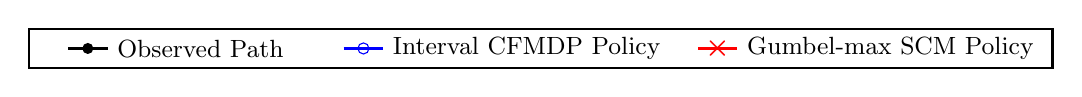
\begin{tikzpicture}[scale=1.0, every node/.style={scale=1.0}]
            \draw[thick, black] (-3, -0.25) rectangle (10, 0.25);
            %
            \draw[black, line width=1pt] (-2.5, 0.0) -- (-2,0.0);
            \fill[black] (-2.25,0.0) circle (2pt); %
            \node[right] at (-2,0.0) {\small Observed Path};
            
            %
            \draw[blue, line width=1pt] (1.0,0.0) -- (1.5,0.0);
            \node[draw=blue, circle, minimum size=4pt, inner sep=0pt] at (1.25,0.0) {}; %
            \node[right] at (1.5,0.0) {\small Interval CFMDP Policy};
            
            %
            \draw[red, line width=1pt] (5.5,0) -- (6,0);
            \node[red] at (5.75,0) {$\boldsymbol{\times}$}; %
            \node[right] at (6,0) {\small Gumbel-max SCM Policy};
        \end{tikzpicture}
    }\\
    %
    \subfigure[\footnotesize Lowest cumulative reward: Interval CFMDP ($312$), Gumbel-max SCM ($312$)]{%
        \resizebox{0.76\columnwidth}{!}{
             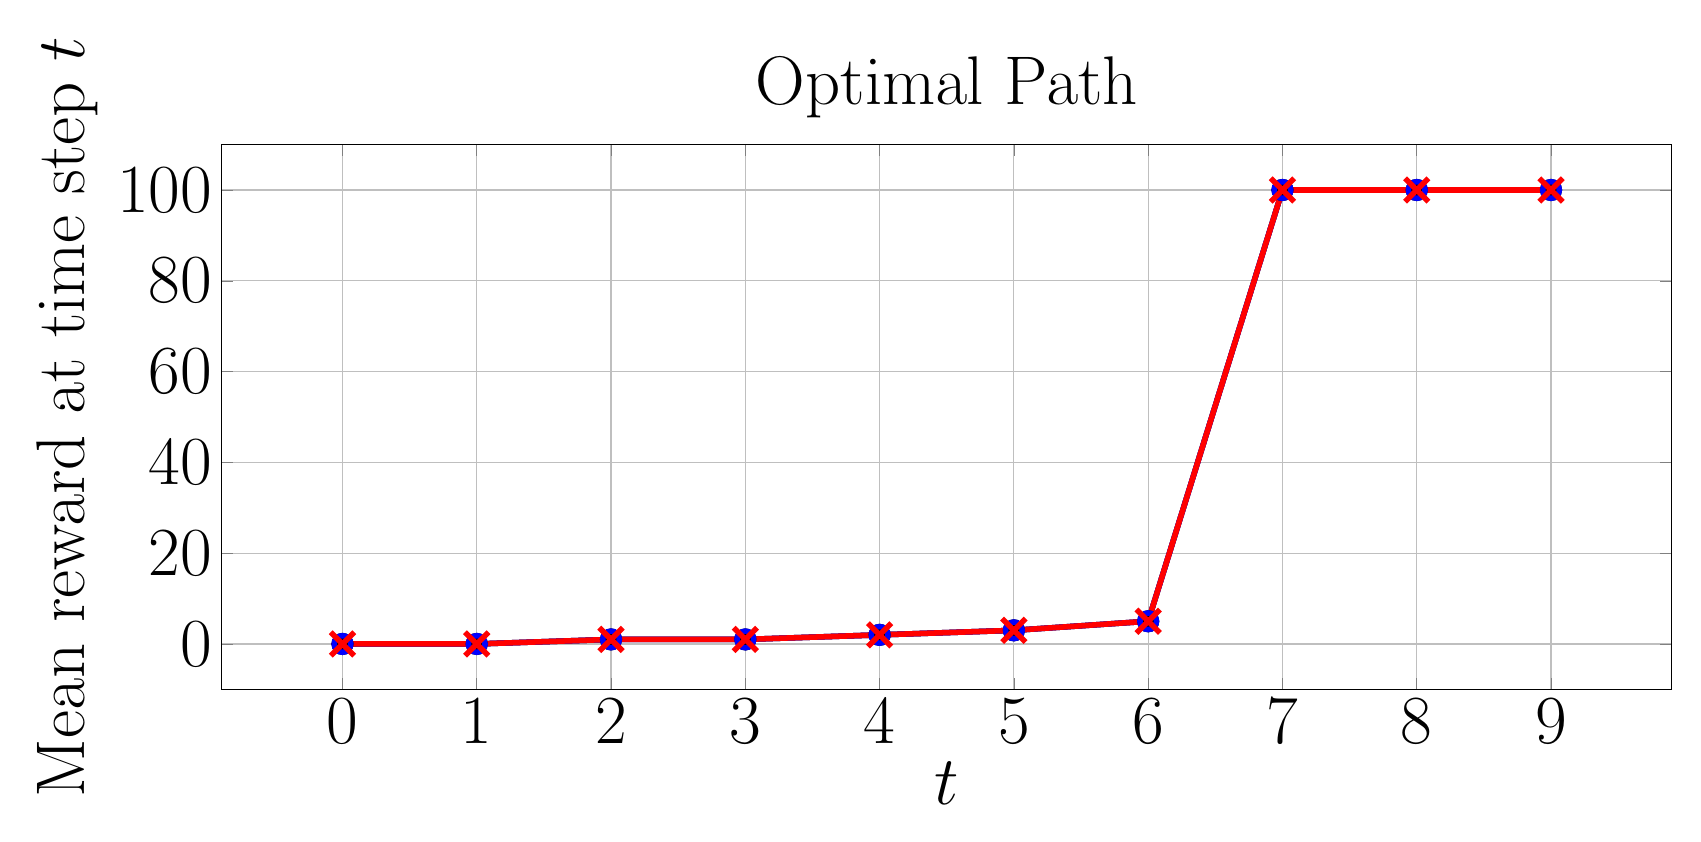
\begin{tikzpicture}
                \begin{axis}[
                    xlabel={$t$},
                    ylabel={Mean reward at time step $t$},
                    title={Optimal Path},
                    grid=both,
                    width=20cm, height=8.5cm,
                    every axis/.style={font=\Huge},
                    %
                ]
                \addplot[
                    color=black, %
                    mark=*, %
                    line width=2pt,
                    mark size=3pt,
                    error bars/.cd,
                    y dir=both, %
                    y explicit, %
                    error bar style={line width=1pt,solid},
                    error mark options={line width=1pt,mark size=4pt,rotate=90}
                ]
                coordinates {
                    (0, 0.0)  +- (0, 0.0)
                    (1, 0.0)  +- (0, 0.0) 
                    (2, 1.0)  +- (0, 0.0) 
                    (3, 1.0)  +- (0, 0.0)
                    (4, 2.0)  +- (0, 0.0)
                    (5, 3.0) +- (0, 0.0)
                    (6, 5.0) +- (0, 0.0)
                    (7, 100.0) +- (0, 0.0)
                    (8, 100.0) +- (0, 0.0)
                    (9, 100.0) +- (0, 0.0)
                };
                %
                \addplot[
                    color=blue, %
                    mark=o, %
                    line width=2pt,
                    mark size=3pt,
                    error bars/.cd,
                    y dir=both, %
                    y explicit, %
                    error bar style={line width=1pt,solid},
                    error mark options={line width=1pt,mark size=4pt,rotate=90}
                ]
                 coordinates {
                    (0, 0.0)  +- (0, 0.0)
                    (1, 0.0)  +- (0, 0.0) 
                    (2, 1.0)  +- (0, 0.0) 
                    (3, 1.0)  +- (0, 0.0)
                    (4, 2.0)  +- (0, 0.0)
                    (5, 3.0) +- (0, 0.0)
                    (6, 5.0) +- (0, 0.0)
                    (7, 100.0) +- (0, 0.0)
                    (8, 100.0) +- (0, 0.0)
                    (9, 100.0) +- (0, 0.0)
                };
                %
                \addplot[
                    color=red, %
                    mark=x, %
                    line width=2pt,
                    mark size=6pt,
                    error bars/.cd,
                    y dir=both, %
                    y explicit, %
                    error bar style={line width=1pt,solid},
                    error mark options={line width=1pt,mark size=4pt,rotate=90}
                ]
                coordinates {
                    (0, 0.0)  +- (0, 0.0)
                    (1, 0.0)  +- (0, 0.0) 
                    (2, 1.0)  +- (0, 0.0) 
                    (3, 1.0)  +- (0, 0.0)
                    (4, 2.0)  +- (0, 0.0)
                    (5, 3.0) +- (0, 0.0)
                    (6, 5.0) +- (0, 0.0)
                    (7, 100.0) +- (0, 0.0)
                    (8, 100.0) +- (0, 0.0)
                    (9, 100.0) +- (0, 0.0)
                };
                \end{axis}
            \end{tikzpicture}
         }
    }
    \hspace{1cm}
    \subfigure[\footnotesize Lowest cumulative reward: Interval CFMDP ($19$), Gumbel-max SCM ($-88$)]{%
         \resizebox{0.76\columnwidth}{!}{
            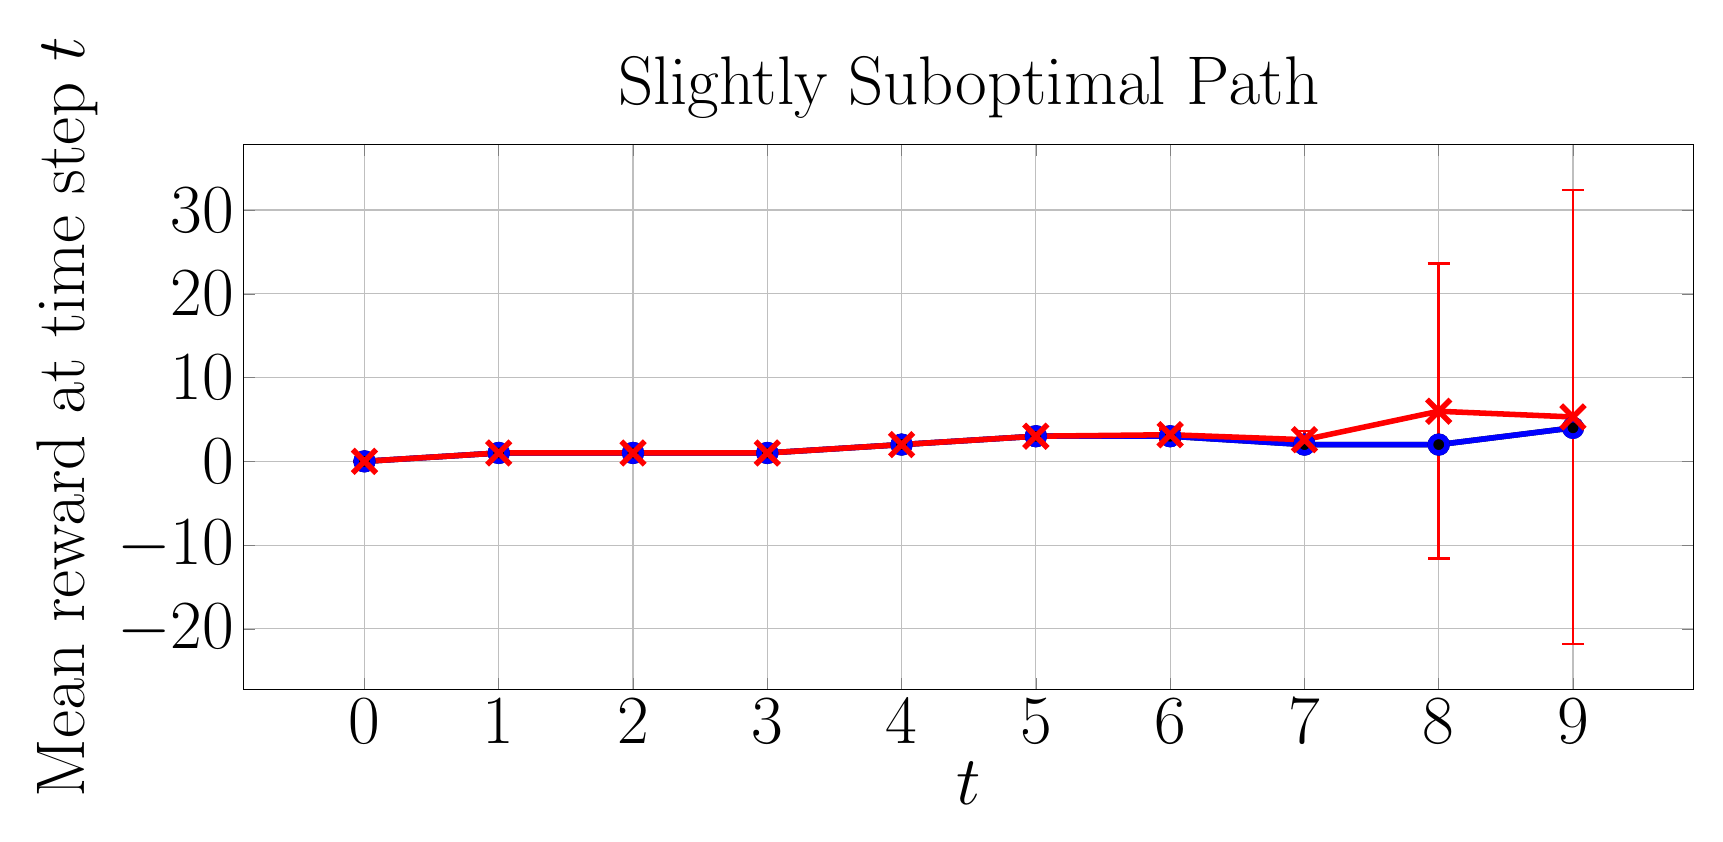
\begin{tikzpicture}
                \begin{axis}[
                    xlabel={$t$},
                    ylabel={Mean reward at time step $t$},
                    title={Slightly Suboptimal Path},
                    grid=both,
                    width=20cm, height=8.5cm,
                    every axis/.style={font=\Huge},
                    %
                ]
                \addplot[
                    color=black, %
                    mark=*, %
                    line width=2pt,
                    mark size=3pt,
                    error bars/.cd,
                    y dir=both, %
                    y explicit, %
                    error bar style={line width=1pt,solid},
                    error mark options={line width=1pt,mark size=4pt,rotate=90}
                ]
              coordinates {
                    (0, 0.0)  +- (0, 0.0)
                    (1, 1.0)  +- (0, 0.0) 
                    (2, 1.0)  +- (0, 0.0) 
                    (3, 1.0)  +- (0, 0.0)
                    (4, 2.0)  +- (0, 0.0)
                    (5, 3.0) +- (0, 0.0)
                    (6, 3.0) +- (0, 0.0)
                    (7, 2.0) +- (0, 0.0)
                    (8, 2.0) +- (0, 0.0)
                    (9, 4.0) +- (0, 0.0)
                };
                %
                \addplot[
                    color=blue, %
                    mark=o, %
                    line width=2pt,
                    mark size=3pt,
                    error bars/.cd,
                    y dir=both, %
                    y explicit, %
                    error bar style={line width=1pt,solid},
                    error mark options={line width=1pt,mark size=4pt,rotate=90}
                ]
              coordinates {
                    (0, 0.0)  +- (0, 0.0)
                    (1, 1.0)  +- (0, 0.0) 
                    (2, 1.0)  +- (0, 0.0) 
                    (3, 1.0)  +- (0, 0.0)
                    (4, 2.0)  +- (0, 0.0)
                    (5, 3.0) +- (0, 0.0)
                    (6, 3.0) +- (0, 0.0)
                    (7, 2.0) +- (0, 0.0)
                    (8, 2.0) +- (0, 0.0)
                    (9, 4.0) +- (0, 0.0)
                };
                %
                \addplot[
                    color=red, %
                    mark=x, %
                    line width=2pt,
                    mark size=6pt,
                    error bars/.cd,
                    y dir=both, %
                    y explicit, %
                    error bar style={line width=1pt,solid},
                    error mark options={line width=1pt,mark size=4pt,rotate=90}
                ]
                coordinates {
                    (0, 0.0)  +- (0, 0.0)
                    (1, 1.0)  +- (0, 0.0) 
                    (2, 1.0)  +- (0, 0.0) 
                    (3, 1.0)  +- (0, 0.0)
                    (4, 2.0)  += (0, 0.0)
                    (5, 3.0)  += (0, 0.0)
                    (6, 3.17847) += (0, 0.62606746) -= (0, 0.62606746)
                    (7, 2.5832885) += (0, 1.04598233) -= (0, 1.04598233)
                    (8, 5.978909) += (0, 17.60137623) -= (0, 17.60137623)
                    (9, 5.297059) += (0, 27.09227512) -= (0, 27.09227512)
                };
                \end{axis}
            \end{tikzpicture}
         }
    }\\[-1.5pt]
    \subfigure[\footnotesize Lowest cumulative reward: Interval CFMDP ($14$), Gumbel-max SCM ($-598$)]{%
         \resizebox{0.76\columnwidth}{!}{
             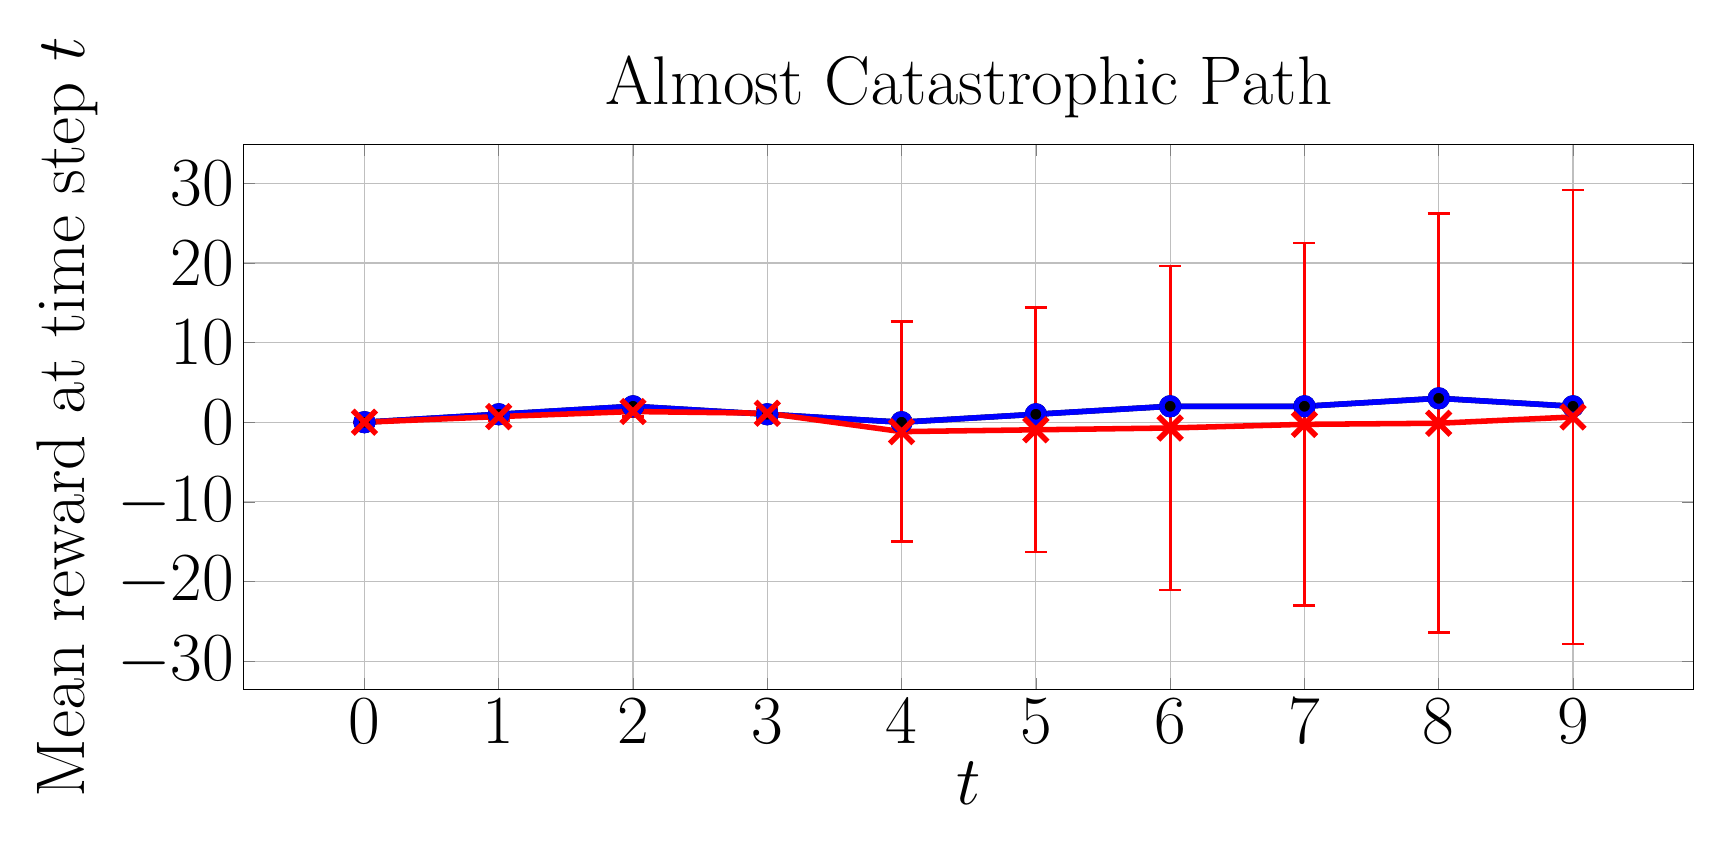
\begin{tikzpicture}
                \begin{axis}[
                    xlabel={$t$},
                    ylabel={Mean reward at time step $t$},
                    title={Almost Catastrophic Path},
                    grid=both,
                    width=20cm, height=8.5cm,
                    every axis/.style={font=\Huge},
                    %
                ]
                \addplot[
                    color=black, %
                    mark=*, %
                    line width=2pt,
                    mark size=3pt,
                    error bars/.cd,
                    y dir=both, %
                    y explicit, %
                    error bar style={line width=1pt,solid},
                    error mark options={line width=1pt,mark size=4pt,rotate=90}
                ]
                coordinates {
                    (0, 0.0)  +- (0, 0.0)
                    (1, 1.0)  +- (0, 0.0) 
                    (2, 2.0)  +- (0, 0.0) 
                    (3, 1.0)  +- (0, 0.0)
                    (4, 0.0)  +- (0, 0.0)
                    (5, 1.0) +- (0, 0.0)
                    (6, 2.0) +- (0, 0.0)
                    (7, 2.0) +- (0, 0.0)
                    (8, 3.0) +- (0, 0.0)
                    (9, 2.0) +- (0, 0.0)
                };
                %
                \addplot[
                    color=blue, %
                    mark=o, %
                    line width=2pt,
                    mark size=3pt,
                    error bars/.cd,
                    y dir=both, %
                    y explicit, %
                    error bar style={line width=1pt,solid},
                    error mark options={line width=1pt,mark size=4pt,rotate=90}
                ]
                coordinates {
                    (0, 0.0)  +- (0, 0.0)
                    (1, 1.0)  +- (0, 0.0) 
                    (2, 2.0)  +- (0, 0.0) 
                    (3, 1.0)  +- (0, 0.0)
                    (4, 0.0)  +- (0, 0.0)
                    (5, 1.0) +- (0, 0.0)
                    (6, 2.0) +- (0, 0.0)
                    (7, 2.0) +- (0, 0.0)
                    (8, 3.0) +- (0, 0.0)
                    (9, 2.0) +- (0, 0.0)
                };
                %
                \addplot[
                    color=red, %
                    mark=x, %
                    line width=2pt,
                    mark size=6pt,
                    error bars/.cd,
                    y dir=both, %
                    y explicit, %
                    error bar style={line width=1pt,solid},
                    error mark options={line width=1pt,mark size=4pt,rotate=90}
                ]
                coordinates {
                    (0, 0.0)  +- (0, 0.0)
                    (1, 0.7065655)  +- (0, 0.4553358) 
                    (2, 1.341673)  +- (0, 0.67091621) 
                    (3, 1.122926)  +- (0, 0.61281824)
                    (4, -1.1821935)  +- (0, 13.82444042)
                    (5, -0.952399)  +- (0, 15.35195457)
                    (6, -0.72672) +- (0, 20.33508414)
                    (7, -0.268983) +- (0, 22.77861454)
                    (8, -0.1310835) +- (0, 26.31013314)
                    (9, 0.65806) +- (0, 28.50670214)
                };
                %
            %
            %
            %
            %
            %
            %
            %
            %
            %
            %
            %
            %
            %
            %
            %
            %
            %
            %
                \end{axis}
            \end{tikzpicture}
         }
    }
    \hspace{1cm}
    \subfigure[\footnotesize Lowest cumulative reward: Interval CFMDP ($-698$), Gumbel-max SCM ($-698$)]{%
         \resizebox{0.76\columnwidth}{!}{
            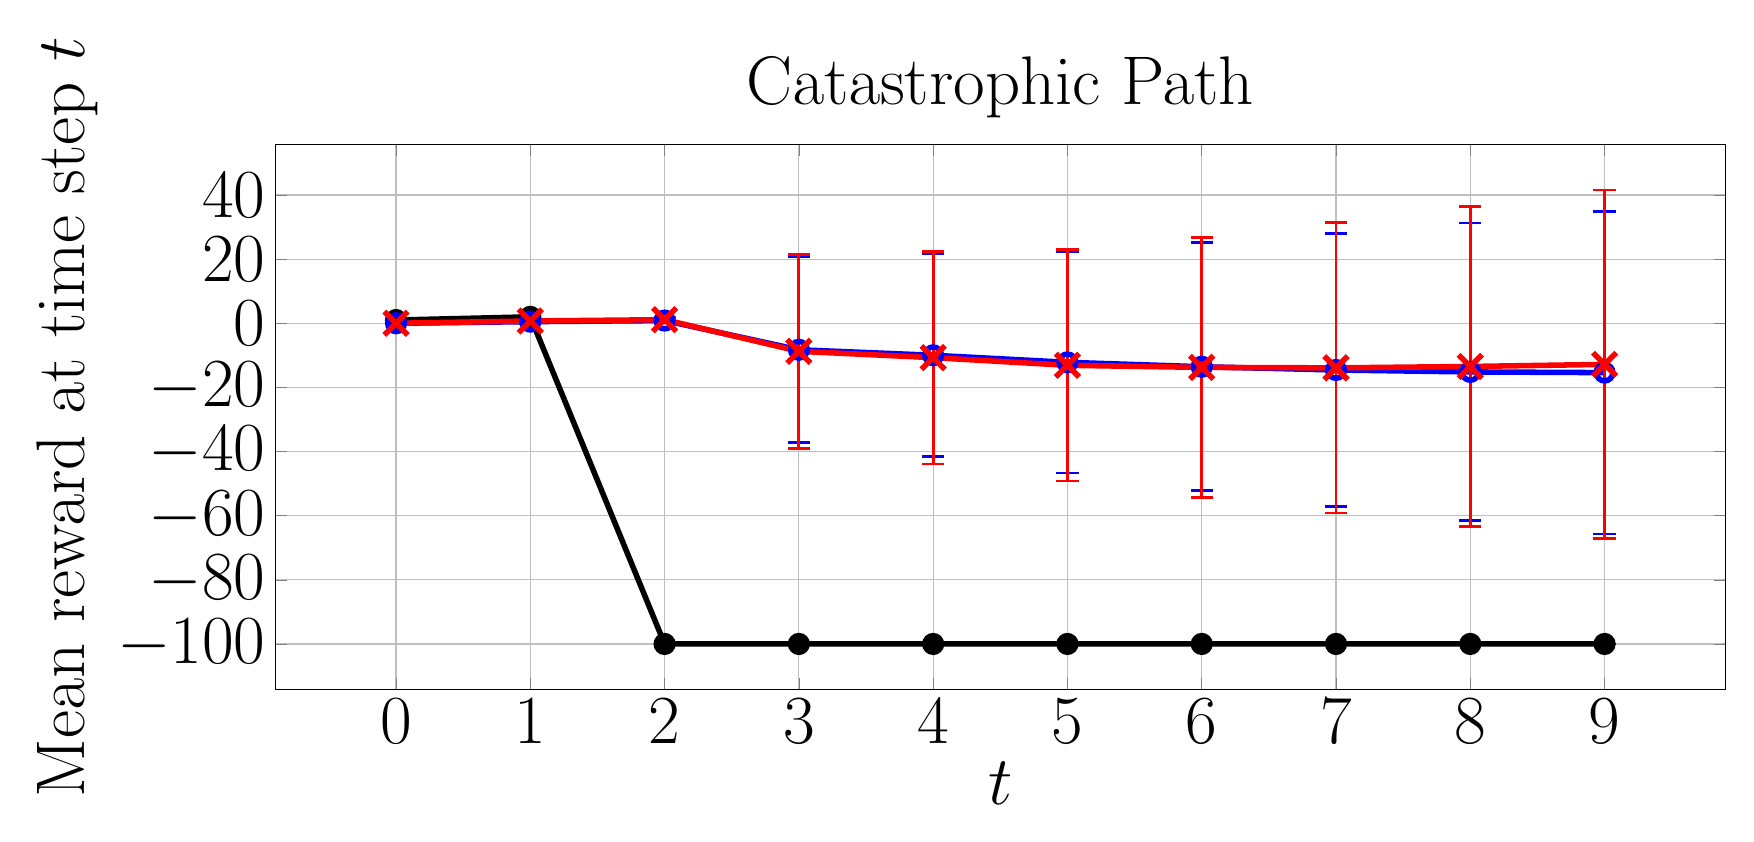
\begin{tikzpicture}
                \begin{axis}[
                    xlabel={$t$},
                    ylabel={Mean reward at time step $t$},
                    title={Catastrophic Path},
                    grid=both,
                    width=20cm, height=8.5cm,
                    every axis/.style={font=\Huge},
                    %
                ]
                \addplot[
                    color=black, %
                    mark=*, %
                    line width=2pt,
                    mark size=3pt,
                    error bars/.cd,
                    y dir=both, %
                    y explicit, %
                    error bar style={line width=1pt,solid},
                    error mark options={line width=1pt,mark size=4pt,rotate=90}
                ]
                coordinates {
                    (0, 1.0)  +- (0, 0.0)
                    (1, 2.0)  +- (0, 0.0) 
                    (2, -100.0)  +- (0, 0.0) 
                    (3, -100.0)  +- (0, 0.0)
                    (4, -100.0)  +- (0, 0.0)
                    (5, -100.0) +- (0, 0.0)
                    (6, -100.0) +- (0, 0.0)
                    (7, -100.0) +- (0, 0.0)
                    (8, -100.0) +- (0, 0.0)
                    (9, -100.0) +- (0, 0.0)
                };
                %
                \addplot[
                    color=blue, %
                    mark=o, %
                    line width=2pt,
                    mark size=3pt,
                    error bars/.cd,
                    y dir=both, %
                    y explicit, %
                    error bar style={line width=1pt,solid},
                    error mark options={line width=1pt,mark size=4pt,rotate=90}
                ]
                coordinates {
                    (0, 0.0)  +- (0, 0.0)
                    (1, 0.504814)  +- (0, 0.49997682) 
                    (2, 0.8439835)  +- (0, 0.76831917) 
                    (3, -8.2709165)  +- (0, 28.93656754)
                    (4, -9.981082)  +- (0, 31.66825363)
                    (5, -12.1776325) +- (0, 34.53463233)
                    (6, -13.556076) +- (0, 38.62845372)
                    (7, -14.574418) +- (0, 42.49603359)
                    (8, -15.1757075) +- (0, 46.41913968)
                    (9, -15.3900395) +- (0, 50.33563368)
                };
                %
                \addplot[
                    color=red, %
                    mark=x, %
                    line width=2pt,
                    mark size=6pt,
                    error bars/.cd,
                    y dir=both, %
                    y explicit, %
                    error bar style={line width=1pt,solid},
                    error mark options={line width=1pt,mark size=4pt,rotate=90}
                ]
                coordinates {
                    (0, 0.0)  +- (0, 0.0)
                    (1, 0.701873)  +- (0, 0.45743556) 
                    (2, 1.1227805)  +- (0, 0.73433129) 
                    (3, -8.7503255)  +- (0, 30.30257976)
                    (4, -10.722092)  +- (0, 33.17618589)
                    (5, -13.10721)  +- (0, 36.0648089)
                    (6, -13.7631645) +- (0, 40.56553451)
                    (7, -13.909043) +- (0, 45.23829402)
                    (8, -13.472517) +- (0, 49.96270296)
                    (9, -12.8278835) +- (0, 54.38618735)
                };
                %
            %
            %
            %
            %
            %
            %
            %
            %
            %
            %
            %
            %
            %
            %
            %
            %
            %
            %
                \end{axis}
            \end{tikzpicture}
         }
    }
    \caption{Average instant reward of CF paths induced by policies on GridWorld $p=0.4$.}
    \label{fig: reward p=0.4}
\end{figure*}

\subsection{Experimental Setup}
To compare policy performance, we measure the average rewards of counterfactual paths induced by our policy and the Gumbel-max policy by uniformly sampling $200$ counterfactual MDPs from the ICFMDP and generating $10,000$ counterfactual paths over each sampled CFMDP. \jl{Since the interval CFMDP depends on the observed path, we select $4$  paths of varying optimality to evaluate how the observed path impacts the performance of both policies: an optimal path, a slightly suboptimal path that could reach the optimal reward with a few changes, a catastrophic path that enters a catastrophic, terminal state with low reward, and an almost catastrophic path that was close to entering a catastrophic state.} When measuring the average probability bound widths and execution time needed to generate the ICFMDPs, we averaged over $20$ randomly generated observed paths
\footnote{Further training details are provided in Appendix \ref{app: training details}, and the code is provided at \href{https://github.com/ddv-lab/robust-cf-inference-in-MDPs}{https://github.com/ddv-lab/robust-cf-inference-in-MDPs}
%
%
.}.

\subsection{GridWorld}
\jl{The GridWorld MDP is a $4 \times 4$ grid where an agent must navigate from the top-left corner to the goal state in the bottom-right corner, avoiding a dangerous terminal state in the centre. At each time step, the agent can move up, down, left, or right, but there is a small probability (controlled by hyper-parameter $p$) of moving in an unintended direction. As the agent nears the goal, the reward for each state increases, culminating in a reward of $+100$ for reaching the goal. Entering the dangerous state results in a penalty of $-100$. We use two versions of GridWorld: a less stochastic version with $p=0.9$ (i.e., $90$\% chance of moving in the chosen direction) and a more stochastic version with $p=0.4$.}

\paragraph{GridWorld ($p=0.9$)}
When $p=0.9$, the counterfactual probability bounds are typically narrow (see Table \ref{tab:nonzero_probs} for average measurements). Consequently, as shown in Figure \ref{fig: reward p=0.9}, both policies are nearly identical and perform similarly well across the optimal, slightly suboptimal, and catastrophic paths.
%
However, for the almost catastrophic path, the interval CFMDP path is more conservative and follows the observed path more closely (as this is where the probability bounds are narrowest), which typically requires one additional step to reach the goal state than the Gumbel-max SCM policy.
%

\paragraph{GridWorld ($p=0.4$)}
\jl{When $p=0.4$, the GridWorld environment becomes more uncertain, increasing the risk of entering the dangerous state even if correct actions are chosen. Thus, as shown in Figure \ref{fig: reward p=0.4}, the interval CFMDP policy adopts a more conservative approach, avoiding deviation from the observed policy if it cannot guarantee higher counterfactual rewards (see the slightly suboptimal and almost catastrophic paths), whereas the Gumbel-max SCM is inconsistent: it can yield higher rewards, but also much lower rewards, reflected in the wide error bars.} For the catastrophic path, both policies must deviate from the observed path to achieve a higher reward and, in this case, perform similarly.
%
%
%
%
\subsection{Sepsis}
The Sepsis MDP \citep{oberst2019counterfactual} simulates trajectories of Sepsis patients. Each state consists of four vital signs (heart rate, blood pressure, oxygen concentration, and glucose levels), categorised as low, normal, or high.
and three treatments that can be toggled on/off at each time step (8 actions in total). Unlike \citet{oberst2019counterfactual}, we scale rewards based on the number of out-of-range vital signs, between $-1000$ (patient dies) and $1000$ (patient discharged). \jl{Like the GridWorld $p=0.4$ experiment, the Sepsis MDP is highly uncertain, as many states are equally likely to lead to optimal and poor outcomes. Thus, as shown in Figure \ref{fig: reward sepsis}, both policies follow the observed optimal and almost catastrophic paths to guarantee rewards are no worse than the observation.} However, improving the catastrophic path requires deviating from the observation. Here, the Gumbel-max SCM policy, on average, performs better than the interval CFMDP policy. But, since both policies have lower bounds clipped at $-1000$, neither policy reliably improves over the observation. In contrast, for the slightly suboptimal path, the interval CFMDP policy performs significantly better, shown by its higher lower bounds. 
Moreover, in these two cases, the worst-case counterfactual path generated by the interval CFMDP policy is better than that of the Gumbel-max SCM policy,
indicating its greater robustness.
%
\begin{figure*}
    \centering
     \resizebox{0.6\textwidth}{!}{
        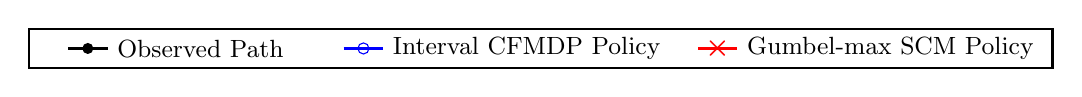
\begin{tikzpicture}[scale=1.0, every node/.style={scale=1.0}]
            \draw[thick, black] (-3, -0.25) rectangle (10, 0.25);
            %
            \draw[black, line width=1pt] (-2.5, 0.0) -- (-2,0.0);
            \fill[black] (-2.25,0.0) circle (2pt); %
            \node[right] at (-2,0.0) {\small Observed Path};
            
            %
            \draw[blue, line width=1pt] (1.0,0.0) -- (1.5,0.0);
            \node[draw=blue, circle, minimum size=4pt, inner sep=0pt] at (1.25,0.0) {}; %
            \node[right] at (1.5,0.0) {\small Interval CFMDP Policy};
            
            %
            \draw[red, line width=1pt] (5.5,0) -- (6,0);
            \node[red] at (5.75,0) {$\boldsymbol{\times}$}; %
            \node[right] at (6,0) {\small Gumbel-max SCM Policy};
        \end{tikzpicture}
    }\\
    \subfigure[\footnotesize Lowest cumulative reward: Interval CFMDP ($8000$), Gumbel-max SCM ($8000$)]{%
         \resizebox{0.76\columnwidth}{!}{
             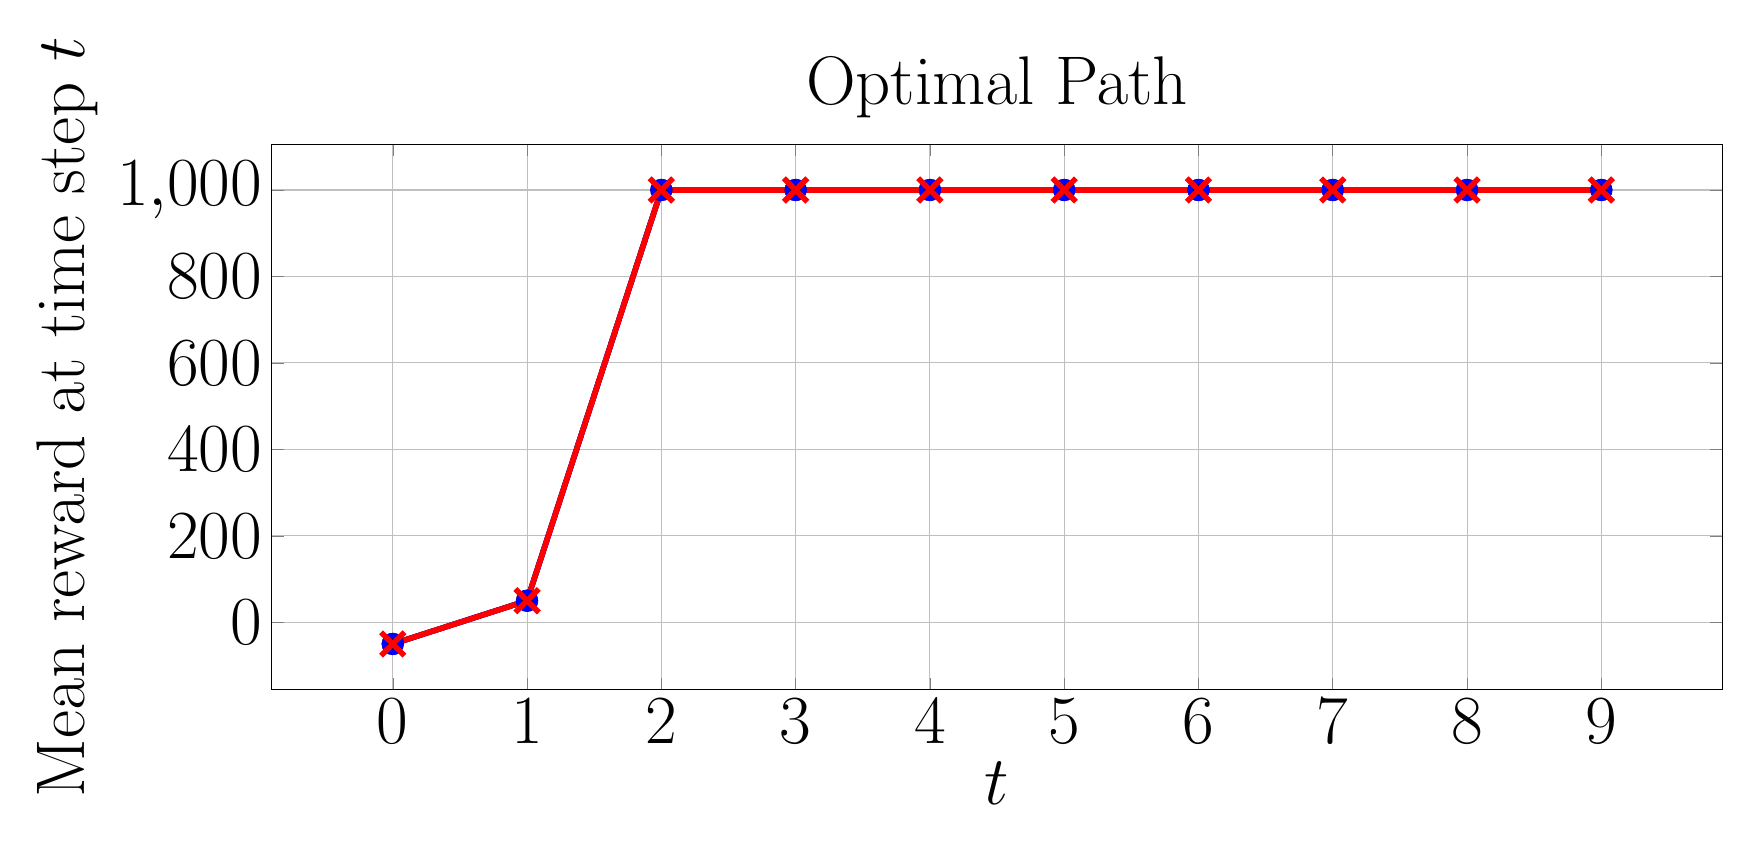
\begin{tikzpicture}
                \begin{axis}[
                    xlabel={$t$},
                    ylabel={Mean reward at time step $t$},
                    title={Optimal Path},
                    grid=both,
                    width=20cm, height=8.5cm,
                    every axis/.style={font=\Huge},
                    %
                ]
                \addplot[
                    color=black, %
                    mark=*, %
                    line width=2pt,
                    mark size=3pt,
                ]
                coordinates {
                    (0, -50.0)
                    (1, 50.0)
                    (2, 1000.0)
                    (3, 1000.0)
                    (4, 1000.0)
                    (5, 1000.0)
                    (6, 1000.0)
                    (7, 1000.0)
                    (8, 1000.0)
                    (9, 1000.0)
                };
                %
                \addplot[
                    color=blue, %
                    mark=o, %
                    line width=2pt,
                    mark size=3pt,
                    error bars/.cd,
                    y dir=both, %
                    y explicit, %
                    error bar style={line width=1pt,solid},
                    error mark options={line width=1pt,mark size=4pt,rotate=90}
                ]
                coordinates {
                    (0, -50.0)  +- (0, 0.0)
                    (1, 50.0)  +- (0, 0.0) 
                    (2, 1000.0)  +- (0, 0.0) 
                    (3, 1000.0)  +- (0, 0.0)
                    (4, 1000.0)  +- (0, 0.0)
                    (5, 1000.0) +- (0, 0.0)
                    (6, 1000.0) +- (0, 0.0)
                    (7, 1000.0) +- (0, 0.0)
                    (8, 1000.0) +- (0, 0.0)
                    (9, 1000.0) +- (0, 0.0)
                };
                %
                \addplot[
                    color=red, %
                    mark=x, %
                    line width=2pt,
                    mark size=6pt,
                    error bars/.cd,
                    y dir=both, %
                    y explicit, %
                    error bar style={line width=1pt,solid},
                    error mark options={line width=1pt,mark size=4pt,rotate=90}
                ]
                coordinates {
                    (0, -50.0)  +- (0, 0.0)
                    (1, 50.0)  +- (0, 0.0) 
                    (2, 1000.0)  +- (0, 0.0) 
                    (3, 1000.0)  +- (0, 0.0)
                    (4, 1000.0)  +- (0, 0.0)
                    (5, 1000.0) +- (0, 0.0)
                    (6, 1000.0) +- (0, 0.0)
                    (7, 1000.0) +- (0, 0.0)
                    (8, 1000.0) +- (0, 0.0)
                    (9, 1000.0) +- (0, 0.0)
                };
                %
                \end{axis}
            \end{tikzpicture}
         }
    }
    \hspace{1cm}
    \subfigure[\footnotesize Lowest cumulative reward: Interval CFMDP ($-5980$), Gumbel-max SCM ($-8000$)]{%
         \resizebox{0.76\columnwidth}{!}{
            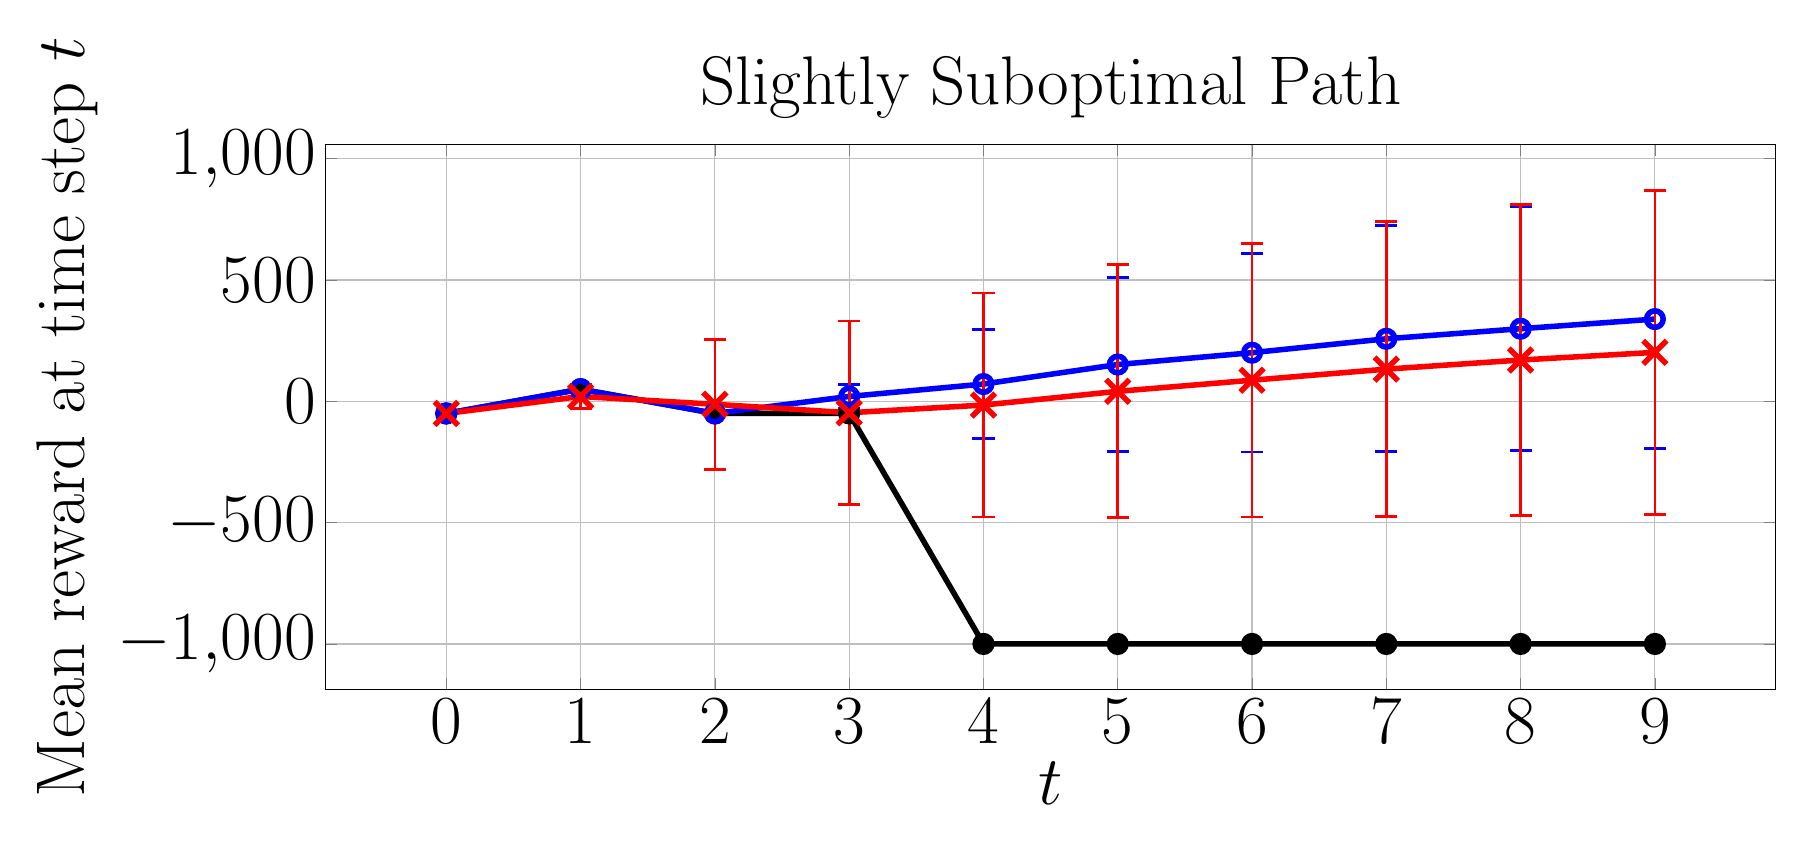
\begin{tikzpicture}
                \begin{axis}[
                    xlabel={$t$},
                    ylabel={Mean reward at time step $t$},
                    title={Slightly Suboptimal Path},
                    grid=both,
                    width=20cm, height=8.5cm,
                    every axis/.style={font=\Huge},
                    %
                ]
               \addplot[
                    color=black, %
                    mark=*, %
                    line width=2pt,
                    mark size=3pt,
                ]
                coordinates {
                    (0, -50.0)
                    (1, 50.0)
                    (2, -50.0)
                    (3, -50.0)
                    (4, -1000.0)
                    (5, -1000.0)
                    (6, -1000.0)
                    (7, -1000.0)
                    (8, -1000.0)
                    (9, -1000.0)
                };
                %
                \addplot[
                    color=blue, %
                    mark=o, %
                    line width=2pt,
                    mark size=3pt,
                    error bars/.cd,
                    y dir=both, %
                    y explicit, %
                    error bar style={line width=1pt,solid},
                    error mark options={line width=1pt,mark size=4pt,rotate=90}
                ]
                coordinates {
                    (0, -50.0)  +- (0, 0.0)
                    (1, 50.0)  +- (0, 0.0) 
                    (2, -50.0)  +- (0, 0.0) 
                    (3, 20.0631)  +- (0, 49.97539413)
                    (4, 71.206585)  +- (0, 226.02033693)
                    (5, 151.60797) +- (0, 359.23292559)
                    (6, 200.40593) +- (0, 408.86185176)
                    (7, 257.77948) +- (0, 466.10372804)
                    (8, 299.237465) +- (0, 501.82579506)
                    (9, 338.9129) +- (0, 532.06124996)
                };
                %
                \addplot[
                    color=red, %
                    mark=x, %
                    line width=2pt,
                    mark size=6pt,
                    error bars/.cd,
                    y dir=both, %
                    y explicit, %
                    error bar style={line width=1pt,solid},
                    error mark options={line width=1pt,mark size=4pt,rotate=90}
                ]
                coordinates {
                    (0, -50.0)  +- (0, 0.0)
                    (1, 20.00736)  +- (0, 49.99786741) 
                    (2, -12.282865)  +- (0, 267.598755) 
                    (3, -47.125995)  +- (0, 378.41755832)
                    (4, -15.381965)  +- (0, 461.77616558)
                    (5, 41.15459) +- (0, 521.53189262)
                    (6, 87.01595) +- (0, 564.22243126 )
                    (7, 132.62376) +- (0, 607.31338037)
                    (8, 170.168145) +- (0, 641.48013693)
                    (9, 201.813135) +- (0, 667.29441777)
                };
                %
                %
                %
                %
                %
                %
                %
                %
                %
                %
                %
                %
                %
                %
                %
                %
                %
                %
                %
                \end{axis}
            \end{tikzpicture}
         }
    }\\[-1.5pt]
    \subfigure[\footnotesize Lowest cumulative reward: Interval CFMDP ($100$), Gumbel-max SCM ($100$)]{%
         \resizebox{0.76\columnwidth}{!}{
             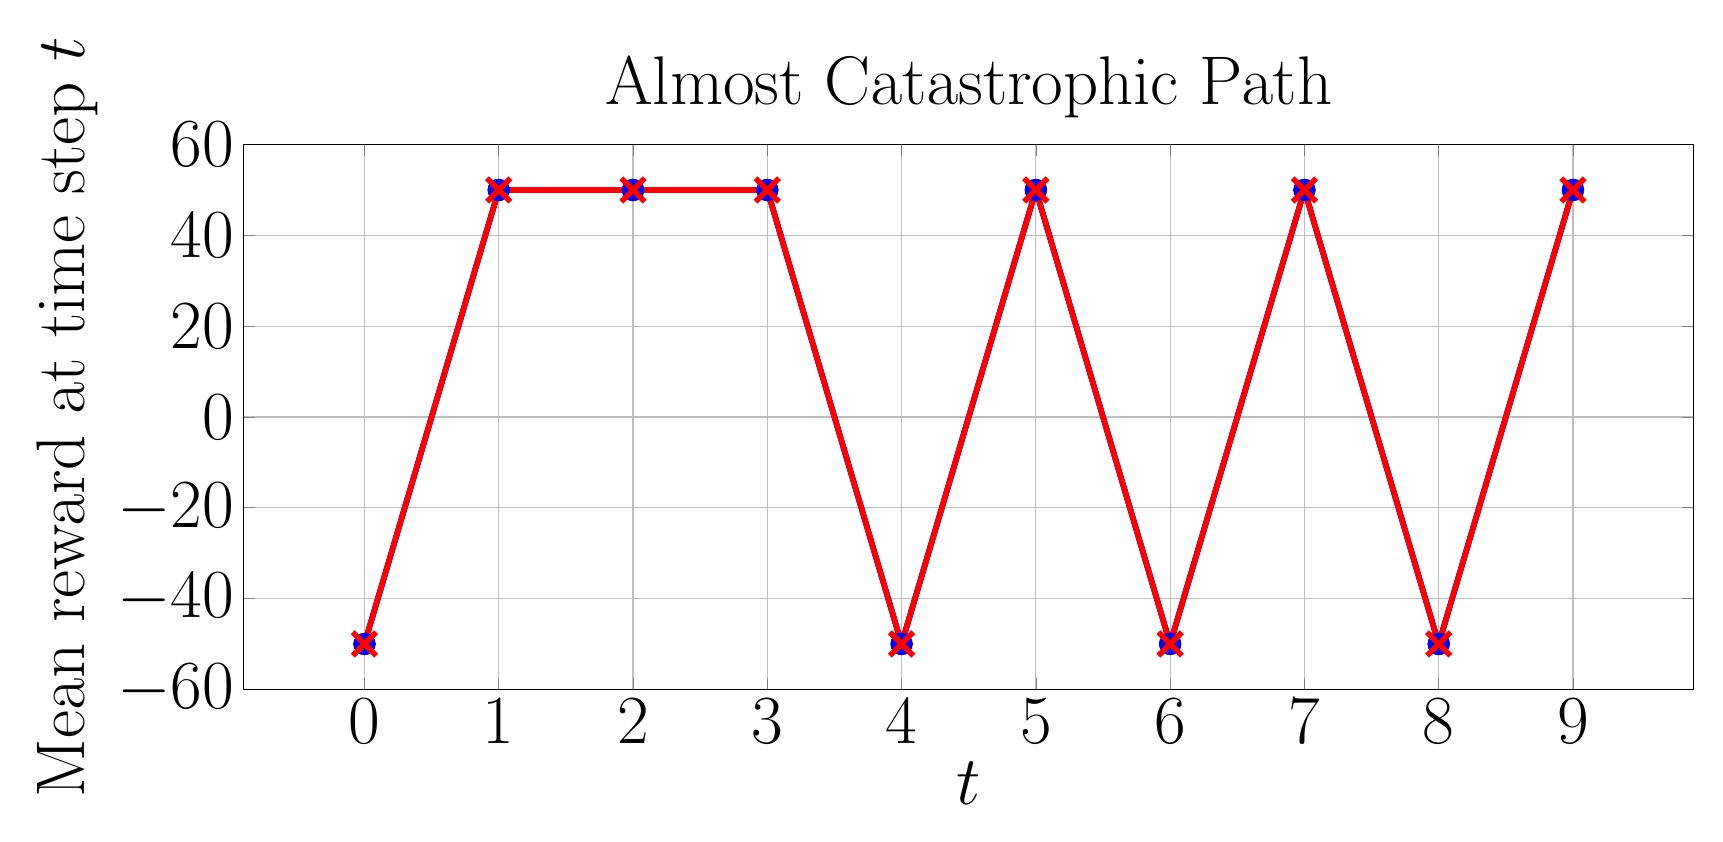
\begin{tikzpicture}
                \begin{axis}[
                    xlabel={$t$},
                    ylabel={Mean reward at time step $t$},
                    title={Almost Catastrophic Path},
                    grid=both,
                    every axis/.style={font=\Huge},
                    width=20cm, height=8.5cm,
                    %
                ]
               \addplot[
                    color=black, %
                    mark=*, %
                    line width=2pt,
                    mark size=3pt,
                ]
                coordinates {
                    (0, -50.0)
                    (1, 50.0)
                    (2, 50.0)
                    (3, 50.0)
                    (4, -50.0)
                    (5, 50.0)
                    (6, -50.0)
                    (7, 50.0)
                    (8, -50.0)
                    (9, 50.0)
                };
                %
                %
                \addplot[
                    color=blue, %
                    mark=o, %
                    line width=2pt,
                    mark size=3pt,
                    error bars/.cd,
                    y dir=both, %
                    y explicit, %
                    error bar style={line width=1pt,solid},
                    error mark options={line width=1pt,mark size=4pt,rotate=90}
                ]
                coordinates {
                    (0, -50.0)  +- (0, 0.0)
                    (1, 50.0)  +- (0, 0.0) 
                    (2, 50.0)  +- (0, 0.0) 
                    (3, 50.0)  +- (0, 0.0)
                    (4, -50.0)  +- (0, 0.0)
                    (5, 50.0) +- (0, 0.0)
                    (6, -50.0) +- (0, 0.0)
                    (7, 50.0) +- (0, 0.0)
                    (8, -50.0) +- (0, 0.0)
                    (9, 50.0) +- (0, 0.0)
                };
                %
                \addplot[
                    color=red, %
                    mark=x, %
                    line width=2pt,
                    mark size=6pt,
                    error bars/.cd,
                    y dir=both, %
                    y explicit, %
                    error bar style={line width=1pt,solid},
                    error mark options={line width=1pt,mark size=4pt,rotate=90}
                ]
                coordinates {
                    (0, -50.0)  +- (0, 0.0)
                    (1, 50.0)  +- (0, 0.0) 
                    (2, 50.0)  +- (0, 0.0) 
                    (3, 50.0)  +- (0, 0.0)
                    (4, -50.0)  +- (0, 0.0)
                    (5, 50.0) +- (0, 0.0)
                    (6, -50.0) +- (0, 0.0)
                    (7, 50.0) +- (0, 0.0)
                    (8, -50.0) +- (0, 0.0)
                    (9, 50.0) +- (0, 0.0)
                };
                %
                %
                %
                %
                %
                %
                %
                %
                %
                %
                %
                %
                %
                %
                %
                %
                %
                %
                %
                \end{axis}
            \end{tikzpicture}
         }
    }
    \hspace{1cm}
    \subfigure[\footnotesize Lowest cumulative reward: Interval CFMDP ($-7150$), Gumbel-max SCM ($-9050$)]{%
         \resizebox{0.76\columnwidth}{!}{
            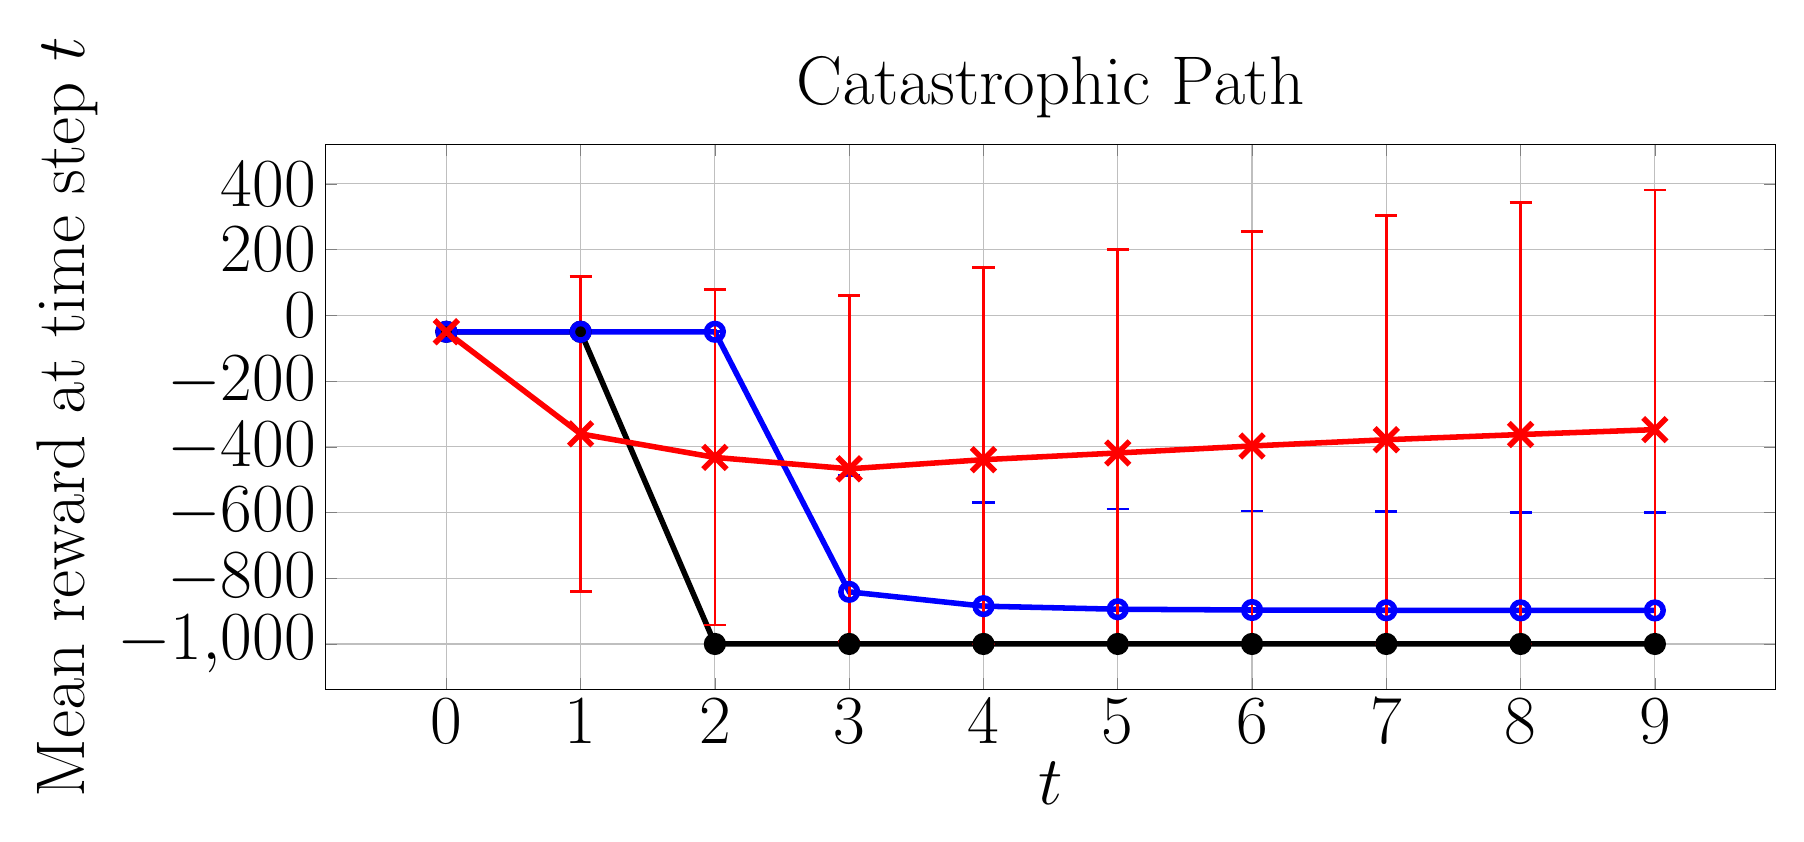
\begin{tikzpicture}
                \begin{axis}[
                    xlabel={$t$},
                    ylabel={Mean reward at time step $t$},
                    title={Catastrophic Path},
                    grid=both,
                    width=20cm, height=8.5cm,
                    every axis/.style={font=\Huge},
                    %
                ]
               \addplot[
                    color=black, %
                    mark=*, %
                    line width=2pt,
                    mark size=3pt,
                ]
                coordinates {
                    (0, -50.0)
                    (1, -50.0)
                    (2, -1000.0)
                    (3, -1000.0)
                    (4, -1000.0)
                    (5, -1000.0)
                    (6, -1000.0)
                    (7, -1000.0)
                    (8, -1000.0)
                    (9, -1000.0)
                };
                %
                %
                \addplot[
                    color=blue, %
                    mark=o, %
                    line width=2pt,
                    mark size=3pt,
                    error bars/.cd,
                    y dir=both, %
                    y explicit, %
                    error bar style={line width=1pt,solid},
                    error mark options={line width=1pt,mark size=4pt,rotate=90}
                ]
                coordinates {
                    (0, -50.0)  +- (0, 0.0)
                    (1, -50.0)  +- (0, 0.0) 
                    (2, -50.0)  +- (0, 0.0) 
                    (3, -841.440725)  += (0, 354.24605512) -= (0, 158.559275)
                    (4, -884.98225)  += (0, 315.37519669) -= (0, 115.01775)
                    (5, -894.330425) += (0, 304.88572805) -= (0, 105.669575)
                    (6, -896.696175) += (0, 301.19954514) -= (0, 103.303825)
                    (7, -897.4635) += (0, 299.61791279) -= (0, 102.5365)
                    (8, -897.77595) += (0, 298.80392585) -= (0, 102.22405)
                    (9, -897.942975) += (0, 298.32920557) -= (0, 102.057025)
                };
                %
                \addplot[
                    color=red, %
                    mark=x, %
                    line width=2pt,
                    mark size=6pt,
                    error bars/.cd,
                    y dir=both, %
                    y explicit, %
                    error bar style={line width=1pt,solid},
                    error mark options={line width=1pt,mark size=4pt,rotate=90}
                ]
            coordinates {
                    (0, -50.0)  +- (0, 0.0)
                    (1, -360.675265)  +- (0, 479.39812699) 
                    (2, -432.27629)  +- (0, 510.38620897) 
                    (3, -467.029545)  += (0, 526.36009628) -= (0, 526.36009628)
                    (4, -439.17429)  += (0, 583.96638919) -= (0, 560.82571)
                    (5, -418.82704) += (0, 618.43027478) -= (0, 581.17296)
                    (6, -397.464895) += (0, 652.67322574) -= (0, 602.535105)
                    (7, -378.49052) += (0, 682.85407033) -= (0, 621.50948)
                    (8, -362.654195) += (0, 707.01412023) -= (0, 637.345805)
                    (9, -347.737935) += (0, 729.29076479) -= (0, 652.262065)
                };
                %
                %
                %
                %
                %
                %
                %
                %
                %
                %
                %
                %
                %
                %
                %
                %
                %
                %
                %
                \end{axis}
            \end{tikzpicture}
         }
    }
    \caption{Average instant reward of CF paths induced by policies on Sepsis.}
    \label{fig: reward sepsis}
\end{figure*}

%
%
%
\subsection{Interval CFMDP Bounds}
%
%
Table \ref{tab:nonzero_probs} presents the mean counterfactual probability bound widths (excluding transitions where the upper bound is $0$) for each MDP, averaged over 20 observed paths. We compare the bounds under counterfactual stability (CS) and monotonicity (M) assumptions, CS alone, and no assumptions. This shows that the assumptions marginally reduce the bound widths, indicating the assumptions tighten the bounds without excluding too many causal models, as intended.
\renewcommand{\arraystretch}{1}

\begin{table}
\centering
\caption{Mean width of counterfactual probability bounds}
\resizebox{0.8\columnwidth}{!}{%
\begin{tabular}{|c|c|c|c|}
\hline
\multirow{2}{*}{\textbf{Environment}} & \multicolumn{3}{c|}{\textbf{Assumptions}} \\ \cline{2-4}
 & \textbf{CS + M} & \textbf{CS} & \textbf{None\tablefootnote{\jl{Equivalent to \citet{li2024probabilities}'s bounds (see Section \ref{sec: equivalence with Li}).}}} \\ \hline
\textbf{GridWorld} ($p=0.9$) & 0.0817 & 0.0977 & 0.100 \\ \hline
\textbf{GridWorld} ($p=0.4$) & 0.552  & 0.638  & 0.646 \\ \hline
\textbf{Sepsis} & 0.138 & 0.140 & 0.140 \\ \hline
\end{tabular}
}
\label{tab:nonzero_probs}
\end{table}


\subsection{Execution Times}
Table \ref{tab: times} compares the average time needed to generate the interval CFMDP vs.\ the Gumbel-max SCM CFMDP for 20 observations.
The GridWorld algorithms were run single-threaded, while the Sepsis experiments were run in parallel.
Generating the interval CFMDP is significantly faster as it uses exact analytical bounds, whereas the Gumbel-max CFMDP requires sampling from the Gumbel distribution to estimate counterfactual transition probabilities. \jl{Since constructing the counterfactual MDP models is the main bottleneck in both approaches, ours is more efficient overall and suitable for larger MDPs.}
\begin{table}
\centering
\caption{Mean execution time to generate CFMDPs}
\resizebox{0.99\columnwidth}{!}{%
\begin{tabular}{|c|c|c|}
\hline
\multirow{2}{*}{\textbf{Environment}} & \multicolumn{2}{c|}{\textbf{Mean Execution Time (s)}} \\ \cline{2-3} 
                                      & \textbf{Interval CFMDP} & \textbf{Gumbel-max CFMDP} \\ \hline
\textbf{GridWorld ($p=0.9$) }                  & 0.261                   & 56.1                      \\ \hline
\textbf{GridWorld ($p=0.4$)  }                 & 0.336                   & 54.5                      \\ \hline
\textbf{Sepsis}                                 & 688                     & 2940                      \\ \hline
\end{tabular}%
}
\label{tab: times}
\end{table}


%\section*{Impact statement}

This paper proposes that machine learning can and should be used to maximize social welfare. In principle, and by construction, the impact of our proposed framework on society aims to be positive. But our paper also points to the inherent difficulties of identifying, and making formal, what `good for society' is. We lean on the field of welfare economics, which has for decades contended with this challenge, for ideas on how the learning community can begin to approach this daunting task.
However, even if these ideas are conceptually appealing,
the path to practical welfare improvement presents many challenges---%
some expected, others unforseen.
% and will likely include many ups and downs.
For example, we may specify incorrect social welfare functions;
or we may specify them correctly but be unable to optimize them appropriately;
or we may be able to optimize but find that 
our assumptions are wrong, that theory differs from practice,
or that there were other considerations and complexities that we did not take into account.
For this we can look to other related fields---%
such as fairness, privacy, and alignment in machine learning---%
which have taken (and are still taking) similar journeys,
and learn from both their success and mistakes.
% and hope that ours will be similar.

Any discipline that seeks to affect policy should do so with much deliberation and care. Whereas welfare economics was designed with the explicit purpose of supporting (and influencing) policymakers,
machine learning has found itself in a similar position, but likely without any planned intent.
On the one hand, adjusting machine learning to support notions, such as social welfare,
that it was not designed to support initially can prove challenging.
However, and as we argue throughout, we believe that building on top of existing machinery is a more practical approach than to begin from scratch.
The necessity of confronting with welfare consideration can also
be an opportunity---as we can leverage these novel challenges
to make machine learning practice more informed, transparent, responsible, and socially aware.


% At the same time, the novelty of the challenges that welfare considerations present to the field make this an opportunity---%
% for chaning the role of machine learning in society for the better in a manner that is informed, transparent, and aware.



\section{Conclusion}
In this work, we propose a simple yet effective approach, called SMILE, for graph few-shot learning with fewer tasks. Specifically, we introduce a novel dual-level mixup strategy, including within-task and across-task mixup, for enriching the diversity of nodes within each task and the diversity of tasks. Also, we incorporate the degree-based prior information to learn expressive node embeddings. Theoretically, we prove that SMILE effectively enhances the model's generalization performance. Empirically, we conduct extensive experiments on multiple benchmarks and the results suggest that SMILE significantly outperforms other baselines, including both in-domain and cross-domain few-shot settings.
% \smallskip
% \myparagraph{Acknowledgments} We thank the reviewers for their comments.
% The work by Moshe Tennenholtz was supported by funding from the
% European Research Council (ERC) under the European Union's Horizon
% 2020 research and innovation programme (grant agreement 740435).



%\input{system_old}




%\input{hidding_prob.tex}
%\section{Network Issues} \label{sec:network-issues}
This section delves into the network layer's vulnerabilities, pivotal for synchronizing time across digital systems. Such synchronization is vital for applications ranging from digital payments to industrial automation. Yet, it faces threats from \textit{attackers controlling network devices} (on-path attacker) or \textit{possessing privileged access to a victim's local network stack} (off-path attacker).

\subsection{Limited Use of Authentication Mechanisms} Cryptography techniques, used by protocols like NTP~\cite{ntpv4-rfc} and PTP~\cite{ptp-std-doc}, play a critical role in ensuring data integrity and origin authentication of the time-sync traffic, thwarting man-in-the-middle (MITM) attacks. Yet, several issues persist regarding the adoption of these methods making time-sync protocols vulnerable to attacks.


\noindent\textbf{\texttt{I10.} False packet injection.} A MITM adversary can impersonate a genuine time server and send false time-sync packets to the target. These attacks may result from weak assumptions underlying the authentication mechanism adopted by the time-sync protocol. For instance, the reliance of NTP's broadcast mode authentication protocol TESLA~\cite{tesla-cryptography} (also used by PTP~\cite{ptp-std-doc}) on loosely synchronized devices creates a circular dependency between authentication and time-sync~\cite{ntp-replay-drop-attack}, rendering the former useless. Moreover, infiltration of malicious servers in the pool of legitimate time servers is  a genuine concern~\cite{shark-ntp-pool, devil-time-origin}. It is because cryptographic authentication only protects against a MITM attacker and the malicious servers render it ineffective. This allows Kwon et. al., to use a handful of malicious time servers, injected to the NTP pool~\cite{ntpd-pool-project}, to disrupt time-sync clients spread over entire countries~\cite{shark-ntp-pool}. Despite their shortcomings, authentication techniques make packet injection attacks harder. However, the adoption of these mechanisms is not universal. For instance, Huygens~\cite{huygens}, RBS~\cite{Elson2003RBS}, FTSP~\cite{ftsp-2004}, TPSN~\cite{tpsn-2003} do not implement any origin authentication mechanisms and have no protection against packet injection. The severity of the issue is evident from the fact that \textit{RBS, FTSP and TPSN} are among the most cited protocols for time-sync in sensor networks. In contrast, secure time synchronization protocols such as the one introduced by Ganeriwal et. al.~\cite{net-sync-wsn-sec-prot} has received an order of magnitude fewer citations (see table~\ref{tab:time-sync-wsn-citations}). Packet injection is one of the most potent attacks against time-sync protocols and could be used to induce \textit{time travel, warping or just increased uncertainty} (\textbf{\texttt{A1-3}}) in the victim's view of time.

\begin{table}
\scriptsize
\centering
\begin{tabular}{ | c | c | c | c | }
 \hline
  \textbf{Protocol} & \textbf{Authentication} & \textbf{Date Published} & \textbf{Citations} \\
 \hline
 \hline
  RBS~\cite{Elson2003RBS}  & \textit{No} & $2003$ & $3927$   \\
 \hline
   TPSN~\cite{tpsn-2003}  & \textit{No} & $2003$ & $3206$   \\
 \hline
   FTSP~\cite{ftsp-2004}  & \textit{No} & $2004$ & $3052$   \\
 \hline
 \hline
   Secure Time-Sync~\cite{Elson2003RBS}  & \textit{Yes} & $2005$ & $278$   \\
 \hline
\end{tabular}
\caption{One of the earliest time-sync protocols proposed for wireless sensor networks (WSNs). The protocols (RBS, TPSN and FTSP) that do not incorporate authentication mechanisms have received an order of magnitude more citations than the protocol (STS) that make use of cryptography mechanisms. \textit{Source: Google Scholars as of Jan 22, 2024.}}
\label{tab:time-sync-wsn-citations}
\end{table}

\noindent\textbf{\texttt{I11.} Packet modification.} Correct implementation of authentication protocols prevents false packet injection but may not prevent against packet modification. This is best exemplified by PTP, which makes use of authentication~\cite{ptp-std-doc} to protects the PTP packets except the correction field of the packet header. This field allows each network node to update correction field with the packet processing delay. PTP uses this information to achieve better time-sync accuracy by eliminating the variable network delays~\cite{net-sync-ptp-covert-channel}. However, a MITM attacker (on-path or off-path) can add incorrect information to this field and manipulate the PTP client. Jacobs et, al., use this channel to introduce \textit{significant offsets} (\textbf{\texttt{A3}}) to the victim device while \textit{avoiding detection}. They could also induce the victim device to change its clock frequency (\textbf{\textit{A2}}), resulting in an even larger time deviation from the time server~\cite{net-sync-ptp-covert-channel}. We note that this attack is not PTP specific, and any time-sync protocol seeking network delay information may be subject to this attack. Finally, we also note that this technique is less sophisticated as it does not require by-passing authentication requires.

\noindent\textbf{\texttt{I12.} Packet replay.} Authentication issues discussed in $I10$ can also result in replay attacks. In this attack, the adversary repeatedly sends one or a sequence of pre-recorded time server packets to the victim. Packet replay attacks have been successfully demonstrated against NTP broadcast mode~\cite{ntp-replay-drop-attack}. Malhotra et. al. exploited limitations in existing NTP client implementations to keep the victim stuck at a single point in time (\textbf{\texttt{A1}}). They point out that the one-way nature of the time-sync traffic (NTP broadcast mode) enables this attack. It implies that other one-way time synchronization protocols such as RBS~\cite{Elson2003RBS} may also be susceptible to this attack.

\noindent\textbf{\texttt{I13.} Spoofing Wireless Timing Signals.} Time-sync protocols like GPS, ROCS~\cite{ROCS-FM-Beacons}, Syntonizor~\cite{Syntonizor-AC-powerlines} and WizSync~\cite{WizSync-Wifi-Beacons} work using a periodic wireless timing signal that is transmitted directly from the timing source(s) to the clients i.e. over a single hop. These protocols lack authentication mechanisms allowing adversaries to spoof timing signals. This attack is the equivalent to packet manipulation attack on packet exchange based protocols (NTP~\cite{nts-rfc}, PTP~\cite{ptp-std-doc}, FTSP~\cite{ftsp-2004} etc.). Similar to the packet manipulation attacks, an external adversary mimics a trusted timing source but transmits incorrect timing information. It does so by generating a powerful spoof signal, using antenna(s), that can overpower the legitimate signal. Such an attacker often stays \textit{stealthy} while introducing uncertainty in the victim's local clocks~\cite{gps-spoofing-fundamentals} (\textbf{\texttt{A3}}). Satellite based global positing systems (GPS) is a typical target of this attack~\cite{gps-spoofing-21}. However, other time-sync protocols in this category (e.g., ROCS,~\cite{ROCS-FM-Beacons}, WizSync~\cite{WizSync-Wifi-Beacons} and Syntonizor~\cite{Syntonizor-AC-powerlines} etc.) haven't seen significant spoofing attacks due to their limited application. Nevertheless, signal spoofing remains a viable attack option for a motivated adversary.

\subsection{Availability Issues}
Beyond modifying timing packets, time-sync is also affected by just delaying the transmission of the timing information (as discussed in section~\ref{subsec:case-studies}). An adversary may leverage this observation and use unpredictable delays to add errors to the time-sync process or it  may outright block time-sync traffic headed towards the victim. 

\noindent\textbf{\texttt{I14.} Packet delay.} Time synchronization protocols determine the time offset between the server and the client by exchanging packets over the network. These network packets experience delays causing uncertainty in the exchanged timing information and the corresponding offset calculations (see section~\ref{subsec:case-studies}). Time-sync protocols rely heavily on precise network delay measurements to remove this uncertainty in the offset estimations. NTP~\cite{ntpv4-rfc} solves this challenge by measuring round trip times (RTTs) and computes network delay as half of the RTT, assuming symmetric delays~\cite{rfc1305}. On the other hand PTP measures the network delays by mandating each processing node to update the PTP packets with its resident delay (see $I11$). While effective under normal network conditions, these delay estimation mechanisms are not robust to adversarial delays. A malicious network node may introduce additional network delays~\footnote{In case of NTP, the server-bound and client-bound packets are delayed by different duration while for PTP the adversary would not update PTP packets with its resident delay} to degrade the synchronization performance. For instance, Annesi et. al. show that delay attacks against PTP can induce errors of several milliseconds, accumulating over time to even larger values under a sustained attacks~\cite{ptp-futile-encryption} (\textbf{\texttt{A2}}). However, vulnerability to delay attacks extend beyond NTP and PTP; virtually all time-sync protocols are susceptible to these attacks.

\noindent\textbf{\texttt{I15.} Packet drop.} 
Intercepting and dropping time-sync packets is a simple yet effective MiTM attack that desynchronizes the victim device from its time server. Facing this \textit{denial-of-service} attack, the victim solely relies on its \textit{local clock} which diverges away from the server time (\textbf{\texttt{A3}}) dictated by the stability of the victim's time source. For low-end systems using inexpensive quartz crystals, the time difference may accumulate to several minutes per day. In contrast, devices using more stable oven-controlled quartz oscillators may experience deviations of only a few seconds in the same period. However, despite its effectiveness, the victim can deduce potential instances of this attack, with relative ease, from sudden unavailability of time-server.

\noindent\textbf{\texttt{I16.} Blocking Wireless Timing Signals.} For single-hop wireless time synchronization (GPS~\cite{gps-spoofing-fundamentals}, ROCS~\cite{ROCS-FM-Beacons}, WizSync~\cite{WizSync-Wifi-Beacons} etc.), denial of service attack takes the form of blocking the wireless timing signal. An adversary achieves this by generating high powered noise in the frequency band used by the wireless timing signal. It requires physical proximity to the target and signal transmission equipment, raising the cost of this attack. Nevertheless, GPS signal blocking techniques have been studied extensively~\cite{gps-jamming-overview} due to ubiquitous use of GPS by defense and civil infrastructure. In principle, other single-hop wireless protocols such as Syntonizor~\cite{Syntonizor-AC-powerlines} and ROC~\cite{ROCS-FM-Beacons} are also vulnerable to these attacks, even though no such attack against them is known.

\subsection{Implementation Issues} In addition to the the communication medium, the end-points of this channel i.e. the applications implementing the time-sync protocol themselves represent an attack surface.

\noindent\textbf{\texttt{I17.} Untrusted time synchronization software.} Applications implementing time-sync protocols may harbor security vulnerabilities of their own. For instance, CVE database lists 98 vulnerabilities, discovered over the years, in the NTP application developed by \textit{NTP.org}~\cite{ntp-cve-details}. This application is used by both the time-sync clients and servers,~\footnote{It is recommended for servers joining the NTP pool project~\cite{ntpd-pool-project}.} and can be exploited by an adversary with access to \textit{privileged execution} on the victim device or \textit{a network connection to the NTP application}. An attack exploiting client side application vulnerability would only affect a single machine, however, the server side exploit would affect time alignment at all of its clients. Further, these attacks may cause the target applications to crash pausing the time-sync service or may just degrade time-sync performance (\textbf{\texttt{A3}}) over longer periods. It is worth pointing out time-sync applications executing in the privileged context present an even bigger risk, as any vulnerability in them could compromise the system beyond time-sync service.
%\definecolor{darkgreen}{rgb}{0.0, 0.5, 0.0}
\definecolor{violet}{rgb}{0.56, 0.0, 1.0}
\section{Evaluation}
We apply our methodology to derive counterfactual policies for various MDPs, addressing three main research questions: (1) how does our policy's performance compare to the Gumbel-max SCM approach; (2) how do the counterfactual stability and monotonicity assumptions impact the probability bounds; and (3) how fast is our approach compared with the Gumbel-max SCM method?

\begin{figure*}
    \centering
    %
    \resizebox{0.6\textwidth}{!}{
        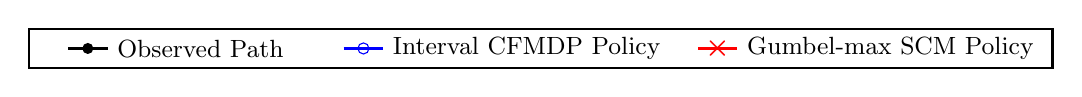
\begin{tikzpicture}[scale=1.0, every node/.style={scale=1.0}]
            \draw[thick, black] (-3, -0.25) rectangle (10, 0.25);
            %
            \draw[black, line width=1pt] (-2.5, 0.0) -- (-2,0.0);
            \fill[black] (-2.25,0.0) circle (2pt); %
            \node[right] at (-2,0.0) {\small Observed Path};
            
            %
            \draw[blue, line width=1pt] (1.0,0.0) -- (1.5,0.0);
            \node[draw=blue, circle, minimum size=4pt, inner sep=0pt] at (1.25,0.0) {}; %
            \node[right] at (1.5,0.0) {\small Interval CFMDP Policy};
            
            %
            \draw[red, line width=1pt] (5.5,0) -- (6,0);
            \node[red] at (5.75,0) {$\boldsymbol{\times}$}; %
            \node[right] at (6,0) {\small Gumbel-max SCM Policy};
        \end{tikzpicture}
    }\\
    %
    \subfigure[\footnotesize Lowest cumulative reward: Interval CFMDP ($312$), Gumbel-max SCM ($312$)]{%
        \resizebox{0.76\columnwidth}{!}{
             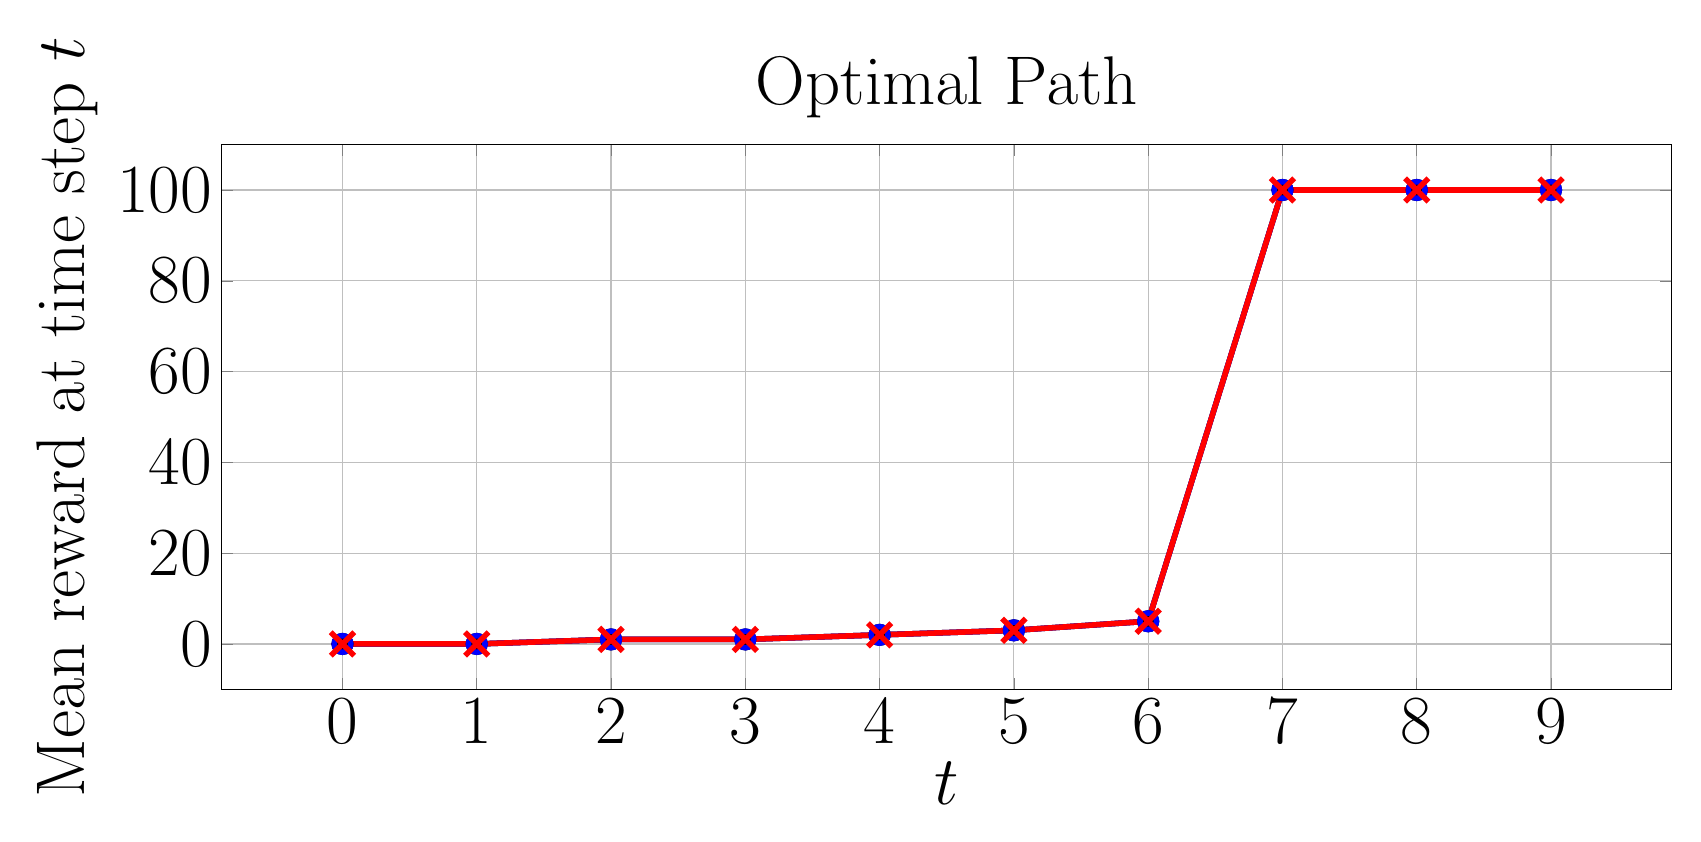
\begin{tikzpicture}
                \begin{axis}[
                    xlabel={$t$},
                    ylabel={Mean reward at time step $t$},
                    title={Optimal Path},
                    grid=both,
                    width=20cm, height=8.5cm,
                    every axis/.style={font=\Huge},
                    %
                ]
                \addplot[
                    color=black, %
                    mark=*, %
                    line width=2pt,
                    mark size=3pt,
                    error bars/.cd,
                    y dir=both, %
                    y explicit, %
                    error bar style={line width=1pt,solid},
                    error mark options={line width=1pt,mark size=4pt,rotate=90}
                ]
                coordinates {
                    (0, 0.0)  +- (0, 0.0)
                    (1, 0.0)  +- (0, 0.0) 
                    (2, 1.0)  +- (0, 0.0) 
                    (3, 1.0)  +- (0, 0.0)
                    (4, 2.0)  +- (0, 0.0)
                    (5, 3.0) +- (0, 0.0)
                    (6, 5.0) +- (0, 0.0)
                    (7, 100.0) +- (0, 0.0)
                    (8, 100.0) +- (0, 0.0)
                    (9, 100.0) +- (0, 0.0)
                };
                %
                \addplot[
                    color=blue, %
                    mark=o, %
                    line width=2pt,
                    mark size=3pt,
                    error bars/.cd,
                    y dir=both, %
                    y explicit, %
                    error bar style={line width=1pt,solid},
                    error mark options={line width=1pt,mark size=4pt,rotate=90}
                ]
                 coordinates {
                    (0, 0.0)  +- (0, 0.0)
                    (1, 0.0)  +- (0, 0.0) 
                    (2, 1.0)  +- (0, 0.0) 
                    (3, 1.0)  +- (0, 0.0)
                    (4, 2.0)  +- (0, 0.0)
                    (5, 3.0) +- (0, 0.0)
                    (6, 5.0) +- (0, 0.0)
                    (7, 100.0) +- (0, 0.0)
                    (8, 100.0) +- (0, 0.0)
                    (9, 100.0) +- (0, 0.0)
                };
                %
                \addplot[
                    color=red, %
                    mark=x, %
                    line width=2pt,
                    mark size=6pt,
                    error bars/.cd,
                    y dir=both, %
                    y explicit, %
                    error bar style={line width=1pt,solid},
                    error mark options={line width=1pt,mark size=4pt,rotate=90}
                ]
                coordinates {
                    (0, 0.0)  +- (0, 0.0)
                    (1, 0.0)  +- (0, 0.0) 
                    (2, 1.0)  +- (0, 0.0) 
                    (3, 1.0)  +- (0, 0.0)
                    (4, 2.0)  +- (0, 0.0)
                    (5, 3.0) +- (0, 0.0)
                    (6, 5.0) +- (0, 0.0)
                    (7, 100.0) +- (0, 0.0)
                    (8, 100.0) +- (0, 0.0)
                    (9, 100.0) +- (0, 0.0)
                };
                \end{axis}
            \end{tikzpicture}
         }
    }
    \hspace{1cm}
    \subfigure[\footnotesize Lowest cumulative reward: Interval CFMDP ($19$), Gumbel-max SCM ($-88$)]{%
         \resizebox{0.76\columnwidth}{!}{
            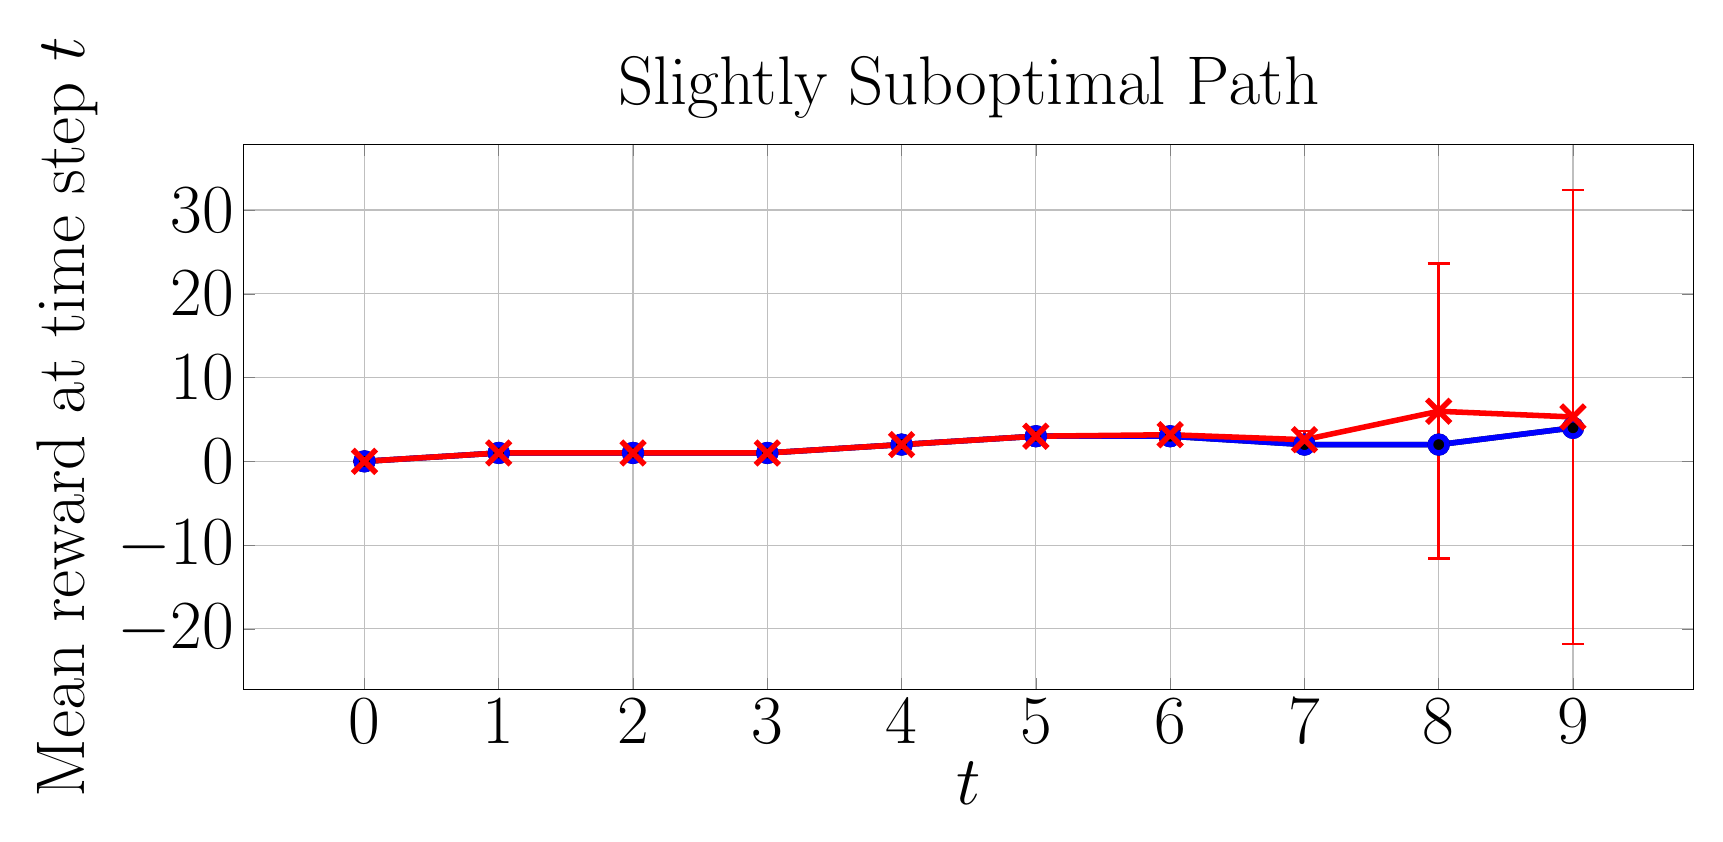
\begin{tikzpicture}
                \begin{axis}[
                    xlabel={$t$},
                    ylabel={Mean reward at time step $t$},
                    title={Slightly Suboptimal Path},
                    grid=both,
                    width=20cm, height=8.5cm,
                    every axis/.style={font=\Huge},
                    %
                ]
                \addplot[
                    color=black, %
                    mark=*, %
                    line width=2pt,
                    mark size=3pt,
                    error bars/.cd,
                    y dir=both, %
                    y explicit, %
                    error bar style={line width=1pt,solid},
                    error mark options={line width=1pt,mark size=4pt,rotate=90}
                ]
              coordinates {
                    (0, 0.0)  +- (0, 0.0)
                    (1, 1.0)  +- (0, 0.0) 
                    (2, 1.0)  +- (0, 0.0) 
                    (3, 1.0)  +- (0, 0.0)
                    (4, 2.0)  +- (0, 0.0)
                    (5, 3.0) +- (0, 0.0)
                    (6, 3.0) +- (0, 0.0)
                    (7, 2.0) +- (0, 0.0)
                    (8, 2.0) +- (0, 0.0)
                    (9, 4.0) +- (0, 0.0)
                };
                %
                \addplot[
                    color=blue, %
                    mark=o, %
                    line width=2pt,
                    mark size=3pt,
                    error bars/.cd,
                    y dir=both, %
                    y explicit, %
                    error bar style={line width=1pt,solid},
                    error mark options={line width=1pt,mark size=4pt,rotate=90}
                ]
              coordinates {
                    (0, 0.0)  +- (0, 0.0)
                    (1, 1.0)  +- (0, 0.0) 
                    (2, 1.0)  +- (0, 0.0) 
                    (3, 1.0)  +- (0, 0.0)
                    (4, 2.0)  +- (0, 0.0)
                    (5, 3.0) +- (0, 0.0)
                    (6, 3.0) +- (0, 0.0)
                    (7, 2.0) +- (0, 0.0)
                    (8, 2.0) +- (0, 0.0)
                    (9, 4.0) +- (0, 0.0)
                };
                %
                \addplot[
                    color=red, %
                    mark=x, %
                    line width=2pt,
                    mark size=6pt,
                    error bars/.cd,
                    y dir=both, %
                    y explicit, %
                    error bar style={line width=1pt,solid},
                    error mark options={line width=1pt,mark size=4pt,rotate=90}
                ]
                coordinates {
                    (0, 0.0)  +- (0, 0.0)
                    (1, 1.0)  +- (0, 0.0) 
                    (2, 1.0)  +- (0, 0.0) 
                    (3, 1.0)  +- (0, 0.0)
                    (4, 2.0)  += (0, 0.0)
                    (5, 3.0)  += (0, 0.0)
                    (6, 3.17847) += (0, 0.62606746) -= (0, 0.62606746)
                    (7, 2.5832885) += (0, 1.04598233) -= (0, 1.04598233)
                    (8, 5.978909) += (0, 17.60137623) -= (0, 17.60137623)
                    (9, 5.297059) += (0, 27.09227512) -= (0, 27.09227512)
                };
                \end{axis}
            \end{tikzpicture}
         }
    }\\[-1.5pt]
    \subfigure[\footnotesize Lowest cumulative reward: Interval CFMDP ($14$), Gumbel-max SCM ($-598$)]{%
         \resizebox{0.76\columnwidth}{!}{
             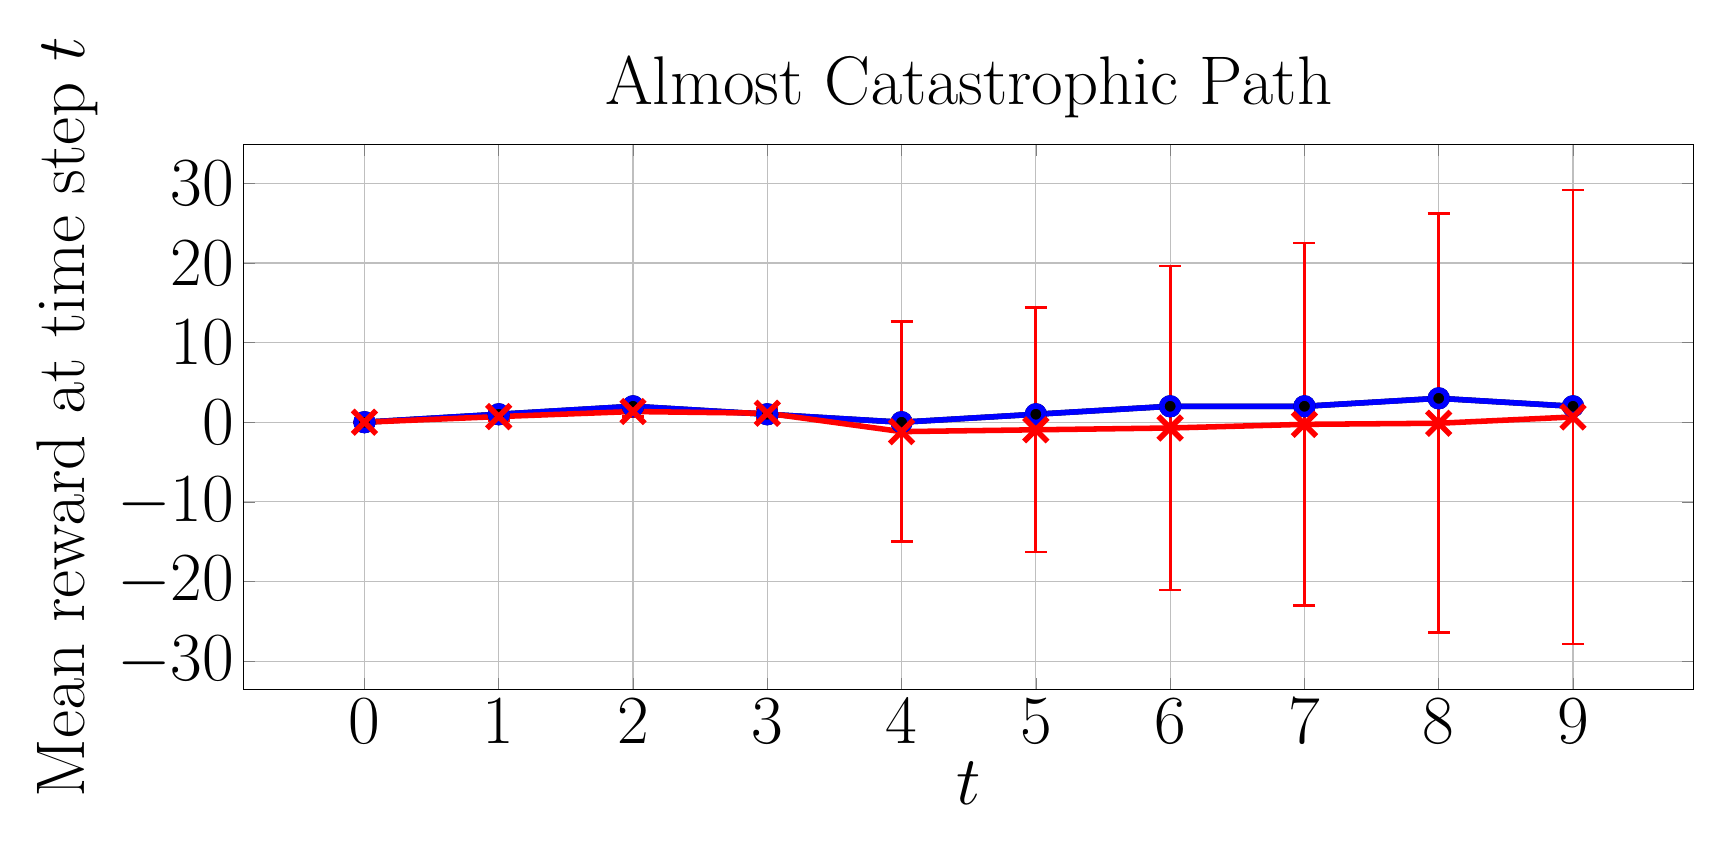
\begin{tikzpicture}
                \begin{axis}[
                    xlabel={$t$},
                    ylabel={Mean reward at time step $t$},
                    title={Almost Catastrophic Path},
                    grid=both,
                    width=20cm, height=8.5cm,
                    every axis/.style={font=\Huge},
                    %
                ]
                \addplot[
                    color=black, %
                    mark=*, %
                    line width=2pt,
                    mark size=3pt,
                    error bars/.cd,
                    y dir=both, %
                    y explicit, %
                    error bar style={line width=1pt,solid},
                    error mark options={line width=1pt,mark size=4pt,rotate=90}
                ]
                coordinates {
                    (0, 0.0)  +- (0, 0.0)
                    (1, 1.0)  +- (0, 0.0) 
                    (2, 2.0)  +- (0, 0.0) 
                    (3, 1.0)  +- (0, 0.0)
                    (4, 0.0)  +- (0, 0.0)
                    (5, 1.0) +- (0, 0.0)
                    (6, 2.0) +- (0, 0.0)
                    (7, 2.0) +- (0, 0.0)
                    (8, 3.0) +- (0, 0.0)
                    (9, 2.0) +- (0, 0.0)
                };
                %
                \addplot[
                    color=blue, %
                    mark=o, %
                    line width=2pt,
                    mark size=3pt,
                    error bars/.cd,
                    y dir=both, %
                    y explicit, %
                    error bar style={line width=1pt,solid},
                    error mark options={line width=1pt,mark size=4pt,rotate=90}
                ]
                coordinates {
                    (0, 0.0)  +- (0, 0.0)
                    (1, 1.0)  +- (0, 0.0) 
                    (2, 2.0)  +- (0, 0.0) 
                    (3, 1.0)  +- (0, 0.0)
                    (4, 0.0)  +- (0, 0.0)
                    (5, 1.0) +- (0, 0.0)
                    (6, 2.0) +- (0, 0.0)
                    (7, 2.0) +- (0, 0.0)
                    (8, 3.0) +- (0, 0.0)
                    (9, 2.0) +- (0, 0.0)
                };
                %
                \addplot[
                    color=red, %
                    mark=x, %
                    line width=2pt,
                    mark size=6pt,
                    error bars/.cd,
                    y dir=both, %
                    y explicit, %
                    error bar style={line width=1pt,solid},
                    error mark options={line width=1pt,mark size=4pt,rotate=90}
                ]
                coordinates {
                    (0, 0.0)  +- (0, 0.0)
                    (1, 0.7065655)  +- (0, 0.4553358) 
                    (2, 1.341673)  +- (0, 0.67091621) 
                    (3, 1.122926)  +- (0, 0.61281824)
                    (4, -1.1821935)  +- (0, 13.82444042)
                    (5, -0.952399)  +- (0, 15.35195457)
                    (6, -0.72672) +- (0, 20.33508414)
                    (7, -0.268983) +- (0, 22.77861454)
                    (8, -0.1310835) +- (0, 26.31013314)
                    (9, 0.65806) +- (0, 28.50670214)
                };
                %
            %
            %
            %
            %
            %
            %
            %
            %
            %
            %
            %
            %
            %
            %
            %
            %
            %
            %
                \end{axis}
            \end{tikzpicture}
         }
    }
    \hspace{1cm}
    \subfigure[\footnotesize Lowest cumulative reward: Interval CFMDP ($-698$), Gumbel-max SCM ($-698$)]{%
         \resizebox{0.76\columnwidth}{!}{
            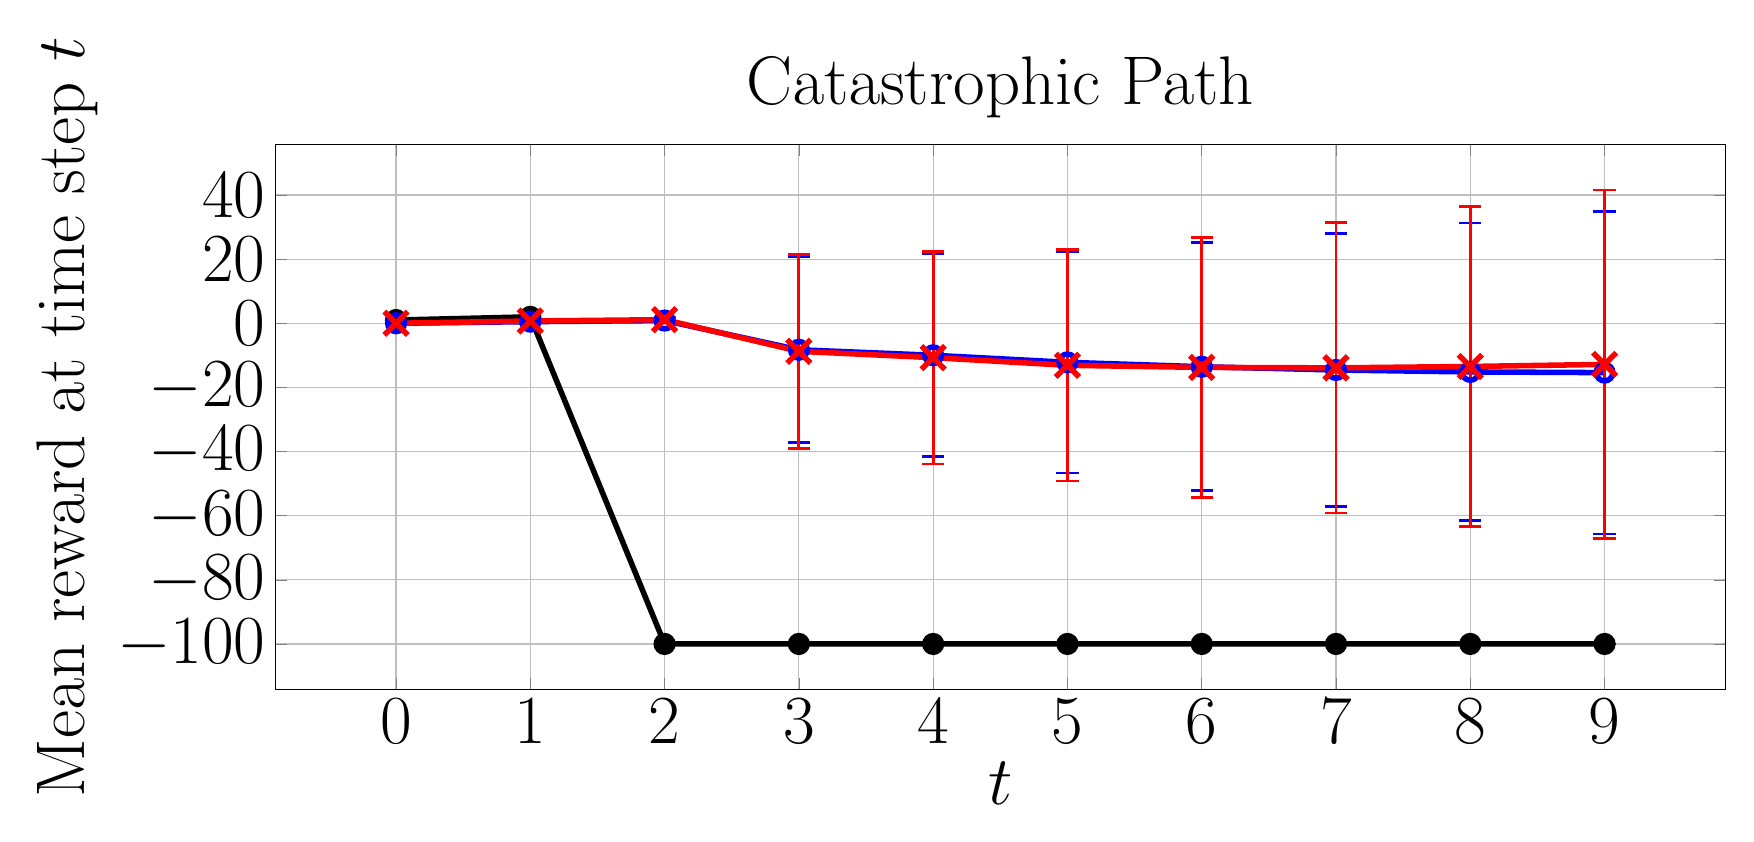
\begin{tikzpicture}
                \begin{axis}[
                    xlabel={$t$},
                    ylabel={Mean reward at time step $t$},
                    title={Catastrophic Path},
                    grid=both,
                    width=20cm, height=8.5cm,
                    every axis/.style={font=\Huge},
                    %
                ]
                \addplot[
                    color=black, %
                    mark=*, %
                    line width=2pt,
                    mark size=3pt,
                    error bars/.cd,
                    y dir=both, %
                    y explicit, %
                    error bar style={line width=1pt,solid},
                    error mark options={line width=1pt,mark size=4pt,rotate=90}
                ]
                coordinates {
                    (0, 1.0)  +- (0, 0.0)
                    (1, 2.0)  +- (0, 0.0) 
                    (2, -100.0)  +- (0, 0.0) 
                    (3, -100.0)  +- (0, 0.0)
                    (4, -100.0)  +- (0, 0.0)
                    (5, -100.0) +- (0, 0.0)
                    (6, -100.0) +- (0, 0.0)
                    (7, -100.0) +- (0, 0.0)
                    (8, -100.0) +- (0, 0.0)
                    (9, -100.0) +- (0, 0.0)
                };
                %
                \addplot[
                    color=blue, %
                    mark=o, %
                    line width=2pt,
                    mark size=3pt,
                    error bars/.cd,
                    y dir=both, %
                    y explicit, %
                    error bar style={line width=1pt,solid},
                    error mark options={line width=1pt,mark size=4pt,rotate=90}
                ]
                coordinates {
                    (0, 0.0)  +- (0, 0.0)
                    (1, 0.504814)  +- (0, 0.49997682) 
                    (2, 0.8439835)  +- (0, 0.76831917) 
                    (3, -8.2709165)  +- (0, 28.93656754)
                    (4, -9.981082)  +- (0, 31.66825363)
                    (5, -12.1776325) +- (0, 34.53463233)
                    (6, -13.556076) +- (0, 38.62845372)
                    (7, -14.574418) +- (0, 42.49603359)
                    (8, -15.1757075) +- (0, 46.41913968)
                    (9, -15.3900395) +- (0, 50.33563368)
                };
                %
                \addplot[
                    color=red, %
                    mark=x, %
                    line width=2pt,
                    mark size=6pt,
                    error bars/.cd,
                    y dir=both, %
                    y explicit, %
                    error bar style={line width=1pt,solid},
                    error mark options={line width=1pt,mark size=4pt,rotate=90}
                ]
                coordinates {
                    (0, 0.0)  +- (0, 0.0)
                    (1, 0.701873)  +- (0, 0.45743556) 
                    (2, 1.1227805)  +- (0, 0.73433129) 
                    (3, -8.7503255)  +- (0, 30.30257976)
                    (4, -10.722092)  +- (0, 33.17618589)
                    (5, -13.10721)  +- (0, 36.0648089)
                    (6, -13.7631645) +- (0, 40.56553451)
                    (7, -13.909043) +- (0, 45.23829402)
                    (8, -13.472517) +- (0, 49.96270296)
                    (9, -12.8278835) +- (0, 54.38618735)
                };
                %
            %
            %
            %
            %
            %
            %
            %
            %
            %
            %
            %
            %
            %
            %
            %
            %
            %
            %
                \end{axis}
            \end{tikzpicture}
         }
    }
    \caption{Average instant reward of CF paths induced by policies on GridWorld $p=0.4$.}
    \label{fig: reward p=0.4}
\end{figure*}

\subsection{Experimental Setup}
To compare policy performance, we measure the average rewards of counterfactual paths induced by our policy and the Gumbel-max policy by uniformly sampling $200$ counterfactual MDPs from the ICFMDP and generating $10,000$ counterfactual paths over each sampled CFMDP. \jl{Since the interval CFMDP depends on the observed path, we select $4$  paths of varying optimality to evaluate how the observed path impacts the performance of both policies: an optimal path, a slightly suboptimal path that could reach the optimal reward with a few changes, a catastrophic path that enters a catastrophic, terminal state with low reward, and an almost catastrophic path that was close to entering a catastrophic state.} When measuring the average probability bound widths and execution time needed to generate the ICFMDPs, we averaged over $20$ randomly generated observed paths
\footnote{Further training details are provided in Appendix \ref{app: training details}, and the code is provided at \href{https://github.com/ddv-lab/robust-cf-inference-in-MDPs}{https://github.com/ddv-lab/robust-cf-inference-in-MDPs}
%
%
.}.

\subsection{GridWorld}
\jl{The GridWorld MDP is a $4 \times 4$ grid where an agent must navigate from the top-left corner to the goal state in the bottom-right corner, avoiding a dangerous terminal state in the centre. At each time step, the agent can move up, down, left, or right, but there is a small probability (controlled by hyper-parameter $p$) of moving in an unintended direction. As the agent nears the goal, the reward for each state increases, culminating in a reward of $+100$ for reaching the goal. Entering the dangerous state results in a penalty of $-100$. We use two versions of GridWorld: a less stochastic version with $p=0.9$ (i.e., $90$\% chance of moving in the chosen direction) and a more stochastic version with $p=0.4$.}

\paragraph{GridWorld ($p=0.9$)}
When $p=0.9$, the counterfactual probability bounds are typically narrow (see Table \ref{tab:nonzero_probs} for average measurements). Consequently, as shown in Figure \ref{fig: reward p=0.9}, both policies are nearly identical and perform similarly well across the optimal, slightly suboptimal, and catastrophic paths.
%
However, for the almost catastrophic path, the interval CFMDP path is more conservative and follows the observed path more closely (as this is where the probability bounds are narrowest), which typically requires one additional step to reach the goal state than the Gumbel-max SCM policy.
%

\paragraph{GridWorld ($p=0.4$)}
\jl{When $p=0.4$, the GridWorld environment becomes more uncertain, increasing the risk of entering the dangerous state even if correct actions are chosen. Thus, as shown in Figure \ref{fig: reward p=0.4}, the interval CFMDP policy adopts a more conservative approach, avoiding deviation from the observed policy if it cannot guarantee higher counterfactual rewards (see the slightly suboptimal and almost catastrophic paths), whereas the Gumbel-max SCM is inconsistent: it can yield higher rewards, but also much lower rewards, reflected in the wide error bars.} For the catastrophic path, both policies must deviate from the observed path to achieve a higher reward and, in this case, perform similarly.
%
%
%
%
\subsection{Sepsis}
The Sepsis MDP \citep{oberst2019counterfactual} simulates trajectories of Sepsis patients. Each state consists of four vital signs (heart rate, blood pressure, oxygen concentration, and glucose levels), categorised as low, normal, or high.
and three treatments that can be toggled on/off at each time step (8 actions in total). Unlike \citet{oberst2019counterfactual}, we scale rewards based on the number of out-of-range vital signs, between $-1000$ (patient dies) and $1000$ (patient discharged). \jl{Like the GridWorld $p=0.4$ experiment, the Sepsis MDP is highly uncertain, as many states are equally likely to lead to optimal and poor outcomes. Thus, as shown in Figure \ref{fig: reward sepsis}, both policies follow the observed optimal and almost catastrophic paths to guarantee rewards are no worse than the observation.} However, improving the catastrophic path requires deviating from the observation. Here, the Gumbel-max SCM policy, on average, performs better than the interval CFMDP policy. But, since both policies have lower bounds clipped at $-1000$, neither policy reliably improves over the observation. In contrast, for the slightly suboptimal path, the interval CFMDP policy performs significantly better, shown by its higher lower bounds. 
Moreover, in these two cases, the worst-case counterfactual path generated by the interval CFMDP policy is better than that of the Gumbel-max SCM policy,
indicating its greater robustness.
%
\begin{figure*}
    \centering
     \resizebox{0.6\textwidth}{!}{
        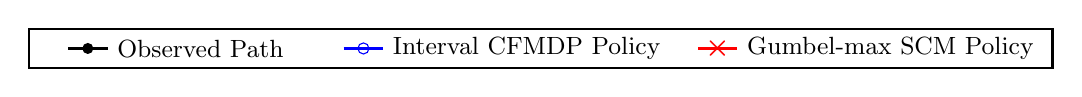
\begin{tikzpicture}[scale=1.0, every node/.style={scale=1.0}]
            \draw[thick, black] (-3, -0.25) rectangle (10, 0.25);
            %
            \draw[black, line width=1pt] (-2.5, 0.0) -- (-2,0.0);
            \fill[black] (-2.25,0.0) circle (2pt); %
            \node[right] at (-2,0.0) {\small Observed Path};
            
            %
            \draw[blue, line width=1pt] (1.0,0.0) -- (1.5,0.0);
            \node[draw=blue, circle, minimum size=4pt, inner sep=0pt] at (1.25,0.0) {}; %
            \node[right] at (1.5,0.0) {\small Interval CFMDP Policy};
            
            %
            \draw[red, line width=1pt] (5.5,0) -- (6,0);
            \node[red] at (5.75,0) {$\boldsymbol{\times}$}; %
            \node[right] at (6,0) {\small Gumbel-max SCM Policy};
        \end{tikzpicture}
    }\\
    \subfigure[\footnotesize Lowest cumulative reward: Interval CFMDP ($8000$), Gumbel-max SCM ($8000$)]{%
         \resizebox{0.76\columnwidth}{!}{
             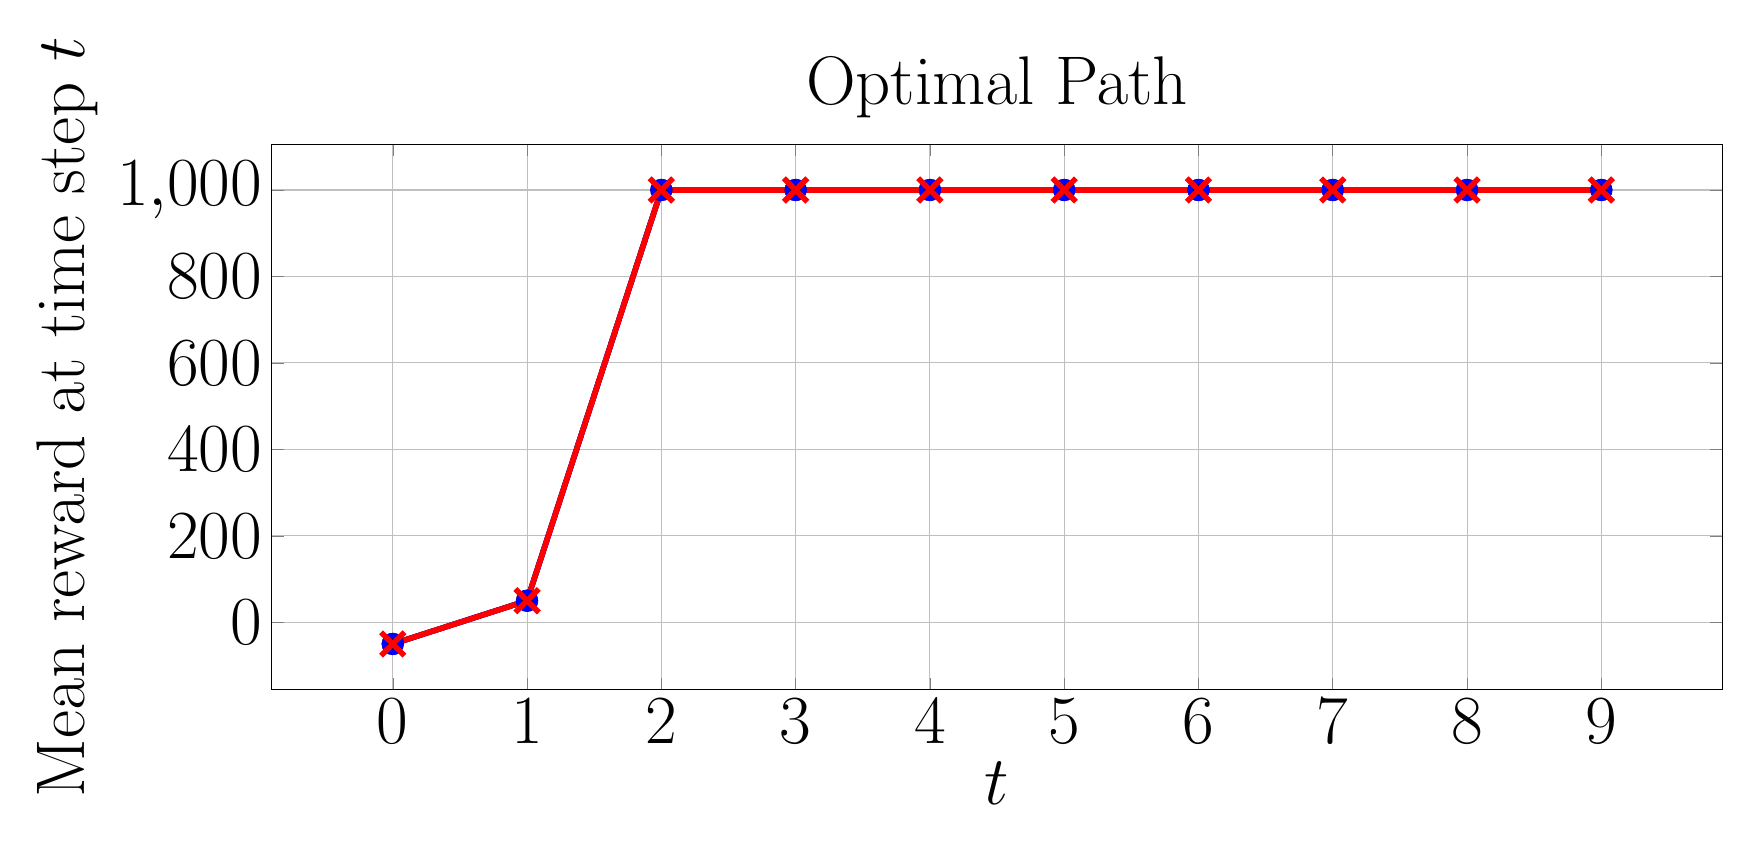
\begin{tikzpicture}
                \begin{axis}[
                    xlabel={$t$},
                    ylabel={Mean reward at time step $t$},
                    title={Optimal Path},
                    grid=both,
                    width=20cm, height=8.5cm,
                    every axis/.style={font=\Huge},
                    %
                ]
                \addplot[
                    color=black, %
                    mark=*, %
                    line width=2pt,
                    mark size=3pt,
                ]
                coordinates {
                    (0, -50.0)
                    (1, 50.0)
                    (2, 1000.0)
                    (3, 1000.0)
                    (4, 1000.0)
                    (5, 1000.0)
                    (6, 1000.0)
                    (7, 1000.0)
                    (8, 1000.0)
                    (9, 1000.0)
                };
                %
                \addplot[
                    color=blue, %
                    mark=o, %
                    line width=2pt,
                    mark size=3pt,
                    error bars/.cd,
                    y dir=both, %
                    y explicit, %
                    error bar style={line width=1pt,solid},
                    error mark options={line width=1pt,mark size=4pt,rotate=90}
                ]
                coordinates {
                    (0, -50.0)  +- (0, 0.0)
                    (1, 50.0)  +- (0, 0.0) 
                    (2, 1000.0)  +- (0, 0.0) 
                    (3, 1000.0)  +- (0, 0.0)
                    (4, 1000.0)  +- (0, 0.0)
                    (5, 1000.0) +- (0, 0.0)
                    (6, 1000.0) +- (0, 0.0)
                    (7, 1000.0) +- (0, 0.0)
                    (8, 1000.0) +- (0, 0.0)
                    (9, 1000.0) +- (0, 0.0)
                };
                %
                \addplot[
                    color=red, %
                    mark=x, %
                    line width=2pt,
                    mark size=6pt,
                    error bars/.cd,
                    y dir=both, %
                    y explicit, %
                    error bar style={line width=1pt,solid},
                    error mark options={line width=1pt,mark size=4pt,rotate=90}
                ]
                coordinates {
                    (0, -50.0)  +- (0, 0.0)
                    (1, 50.0)  +- (0, 0.0) 
                    (2, 1000.0)  +- (0, 0.0) 
                    (3, 1000.0)  +- (0, 0.0)
                    (4, 1000.0)  +- (0, 0.0)
                    (5, 1000.0) +- (0, 0.0)
                    (6, 1000.0) +- (0, 0.0)
                    (7, 1000.0) +- (0, 0.0)
                    (8, 1000.0) +- (0, 0.0)
                    (9, 1000.0) +- (0, 0.0)
                };
                %
                \end{axis}
            \end{tikzpicture}
         }
    }
    \hspace{1cm}
    \subfigure[\footnotesize Lowest cumulative reward: Interval CFMDP ($-5980$), Gumbel-max SCM ($-8000$)]{%
         \resizebox{0.76\columnwidth}{!}{
            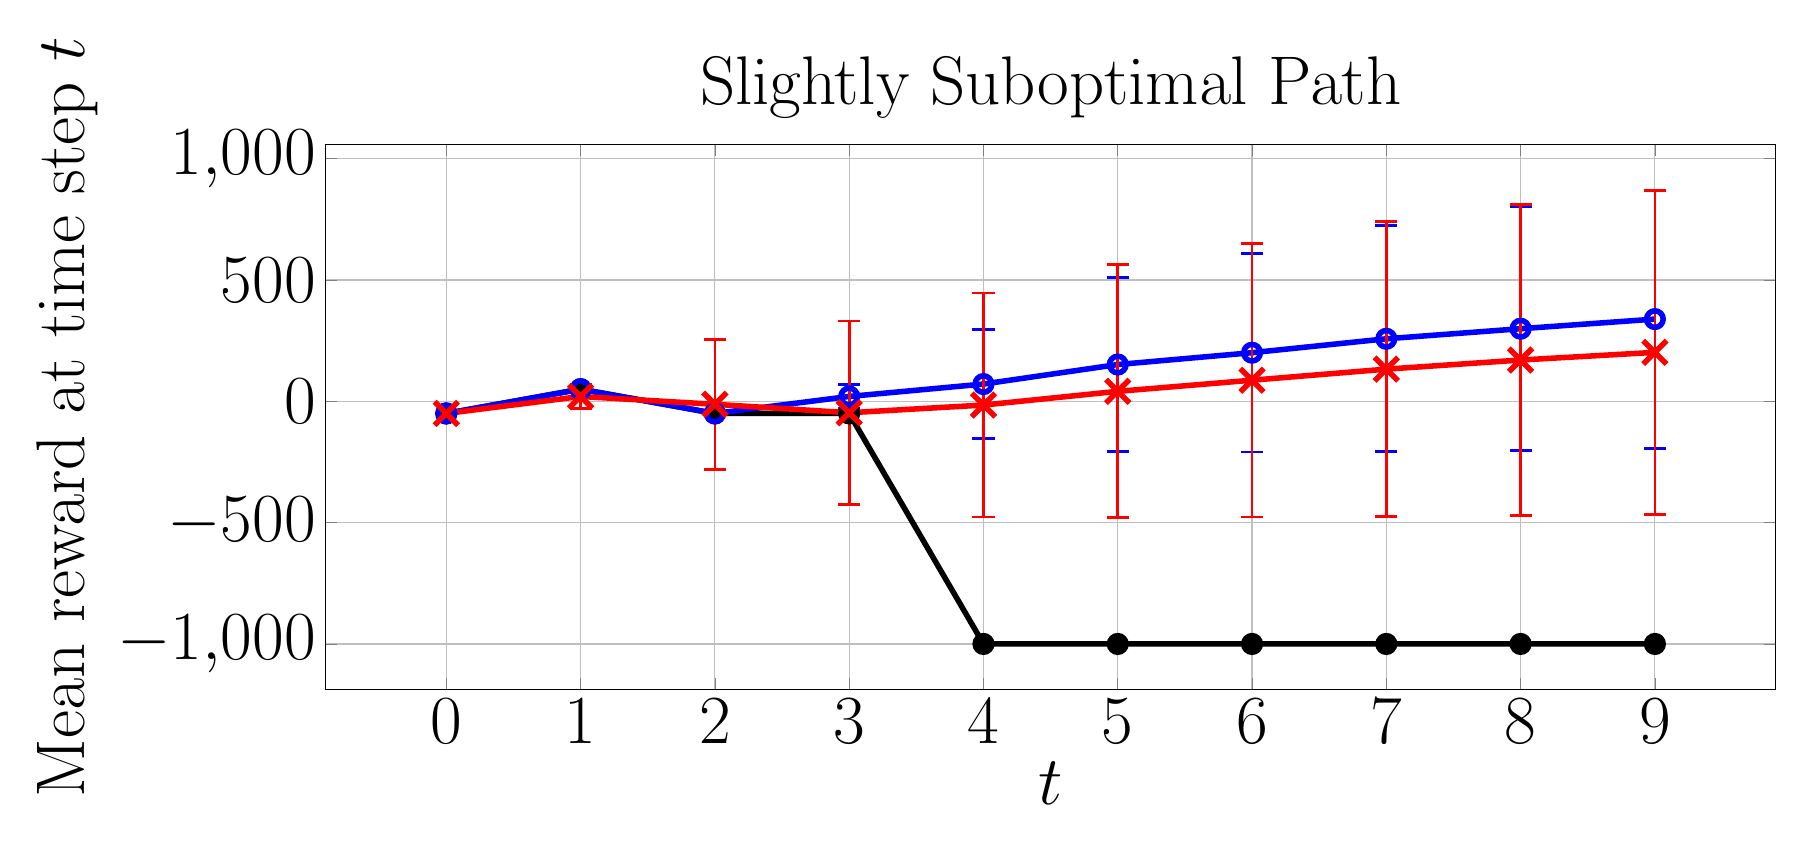
\begin{tikzpicture}
                \begin{axis}[
                    xlabel={$t$},
                    ylabel={Mean reward at time step $t$},
                    title={Slightly Suboptimal Path},
                    grid=both,
                    width=20cm, height=8.5cm,
                    every axis/.style={font=\Huge},
                    %
                ]
               \addplot[
                    color=black, %
                    mark=*, %
                    line width=2pt,
                    mark size=3pt,
                ]
                coordinates {
                    (0, -50.0)
                    (1, 50.0)
                    (2, -50.0)
                    (3, -50.0)
                    (4, -1000.0)
                    (5, -1000.0)
                    (6, -1000.0)
                    (7, -1000.0)
                    (8, -1000.0)
                    (9, -1000.0)
                };
                %
                \addplot[
                    color=blue, %
                    mark=o, %
                    line width=2pt,
                    mark size=3pt,
                    error bars/.cd,
                    y dir=both, %
                    y explicit, %
                    error bar style={line width=1pt,solid},
                    error mark options={line width=1pt,mark size=4pt,rotate=90}
                ]
                coordinates {
                    (0, -50.0)  +- (0, 0.0)
                    (1, 50.0)  +- (0, 0.0) 
                    (2, -50.0)  +- (0, 0.0) 
                    (3, 20.0631)  +- (0, 49.97539413)
                    (4, 71.206585)  +- (0, 226.02033693)
                    (5, 151.60797) +- (0, 359.23292559)
                    (6, 200.40593) +- (0, 408.86185176)
                    (7, 257.77948) +- (0, 466.10372804)
                    (8, 299.237465) +- (0, 501.82579506)
                    (9, 338.9129) +- (0, 532.06124996)
                };
                %
                \addplot[
                    color=red, %
                    mark=x, %
                    line width=2pt,
                    mark size=6pt,
                    error bars/.cd,
                    y dir=both, %
                    y explicit, %
                    error bar style={line width=1pt,solid},
                    error mark options={line width=1pt,mark size=4pt,rotate=90}
                ]
                coordinates {
                    (0, -50.0)  +- (0, 0.0)
                    (1, 20.00736)  +- (0, 49.99786741) 
                    (2, -12.282865)  +- (0, 267.598755) 
                    (3, -47.125995)  +- (0, 378.41755832)
                    (4, -15.381965)  +- (0, 461.77616558)
                    (5, 41.15459) +- (0, 521.53189262)
                    (6, 87.01595) +- (0, 564.22243126 )
                    (7, 132.62376) +- (0, 607.31338037)
                    (8, 170.168145) +- (0, 641.48013693)
                    (9, 201.813135) +- (0, 667.29441777)
                };
                %
                %
                %
                %
                %
                %
                %
                %
                %
                %
                %
                %
                %
                %
                %
                %
                %
                %
                %
                \end{axis}
            \end{tikzpicture}
         }
    }\\[-1.5pt]
    \subfigure[\footnotesize Lowest cumulative reward: Interval CFMDP ($100$), Gumbel-max SCM ($100$)]{%
         \resizebox{0.76\columnwidth}{!}{
             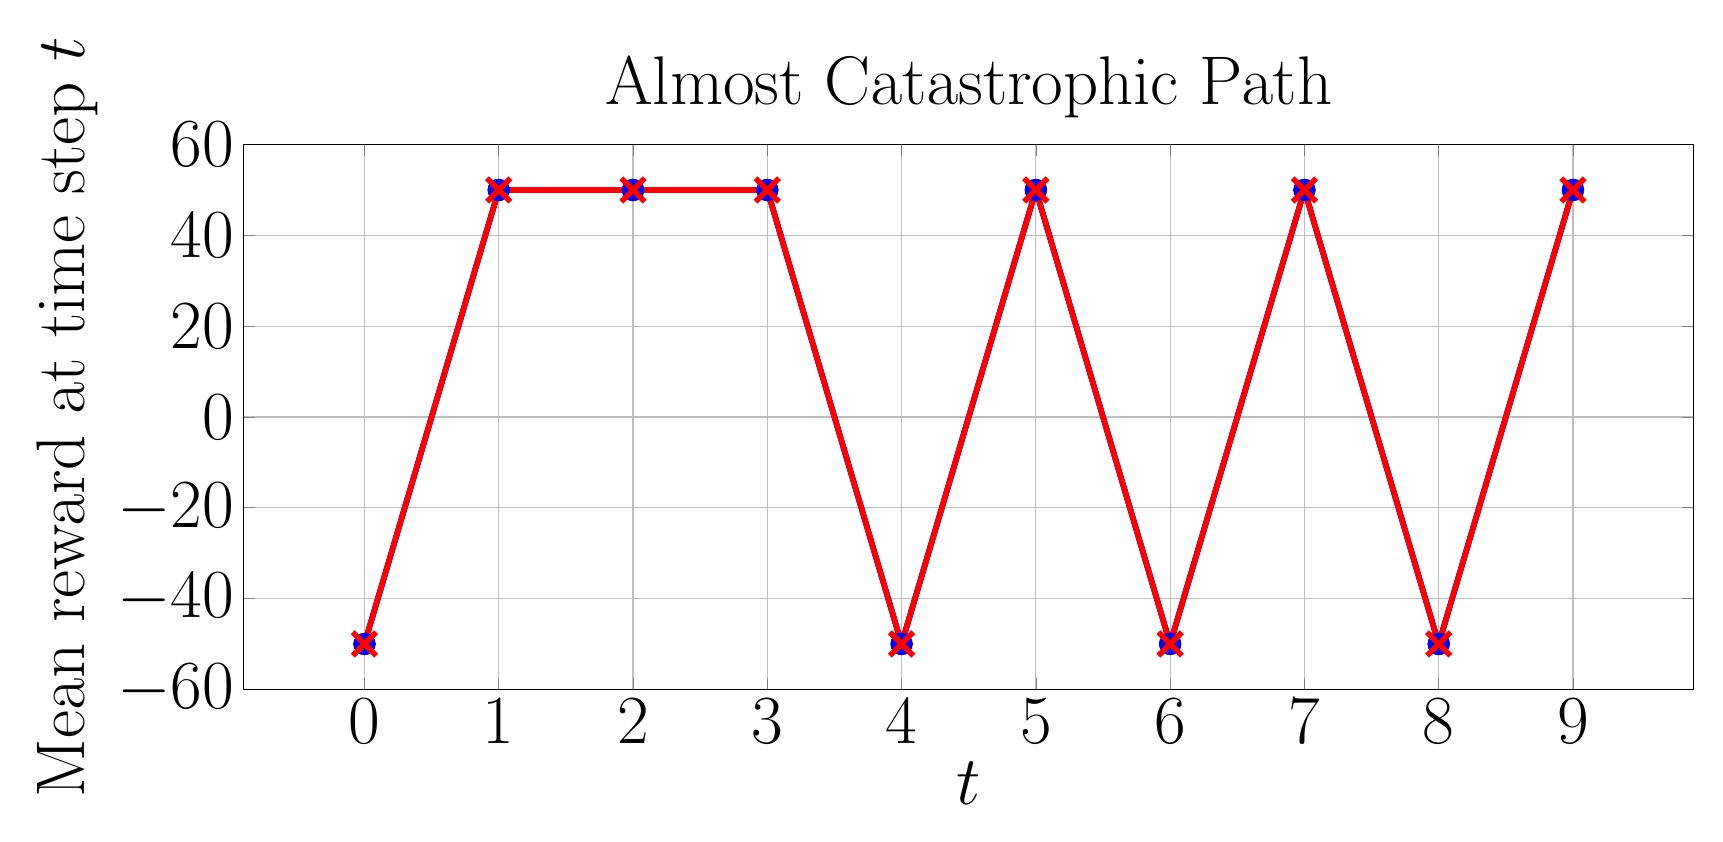
\begin{tikzpicture}
                \begin{axis}[
                    xlabel={$t$},
                    ylabel={Mean reward at time step $t$},
                    title={Almost Catastrophic Path},
                    grid=both,
                    every axis/.style={font=\Huge},
                    width=20cm, height=8.5cm,
                    %
                ]
               \addplot[
                    color=black, %
                    mark=*, %
                    line width=2pt,
                    mark size=3pt,
                ]
                coordinates {
                    (0, -50.0)
                    (1, 50.0)
                    (2, 50.0)
                    (3, 50.0)
                    (4, -50.0)
                    (5, 50.0)
                    (6, -50.0)
                    (7, 50.0)
                    (8, -50.0)
                    (9, 50.0)
                };
                %
                %
                \addplot[
                    color=blue, %
                    mark=o, %
                    line width=2pt,
                    mark size=3pt,
                    error bars/.cd,
                    y dir=both, %
                    y explicit, %
                    error bar style={line width=1pt,solid},
                    error mark options={line width=1pt,mark size=4pt,rotate=90}
                ]
                coordinates {
                    (0, -50.0)  +- (0, 0.0)
                    (1, 50.0)  +- (0, 0.0) 
                    (2, 50.0)  +- (0, 0.0) 
                    (3, 50.0)  +- (0, 0.0)
                    (4, -50.0)  +- (0, 0.0)
                    (5, 50.0) +- (0, 0.0)
                    (6, -50.0) +- (0, 0.0)
                    (7, 50.0) +- (0, 0.0)
                    (8, -50.0) +- (0, 0.0)
                    (9, 50.0) +- (0, 0.0)
                };
                %
                \addplot[
                    color=red, %
                    mark=x, %
                    line width=2pt,
                    mark size=6pt,
                    error bars/.cd,
                    y dir=both, %
                    y explicit, %
                    error bar style={line width=1pt,solid},
                    error mark options={line width=1pt,mark size=4pt,rotate=90}
                ]
                coordinates {
                    (0, -50.0)  +- (0, 0.0)
                    (1, 50.0)  +- (0, 0.0) 
                    (2, 50.0)  +- (0, 0.0) 
                    (3, 50.0)  +- (0, 0.0)
                    (4, -50.0)  +- (0, 0.0)
                    (5, 50.0) +- (0, 0.0)
                    (6, -50.0) +- (0, 0.0)
                    (7, 50.0) +- (0, 0.0)
                    (8, -50.0) +- (0, 0.0)
                    (9, 50.0) +- (0, 0.0)
                };
                %
                %
                %
                %
                %
                %
                %
                %
                %
                %
                %
                %
                %
                %
                %
                %
                %
                %
                %
                \end{axis}
            \end{tikzpicture}
         }
    }
    \hspace{1cm}
    \subfigure[\footnotesize Lowest cumulative reward: Interval CFMDP ($-7150$), Gumbel-max SCM ($-9050$)]{%
         \resizebox{0.76\columnwidth}{!}{
            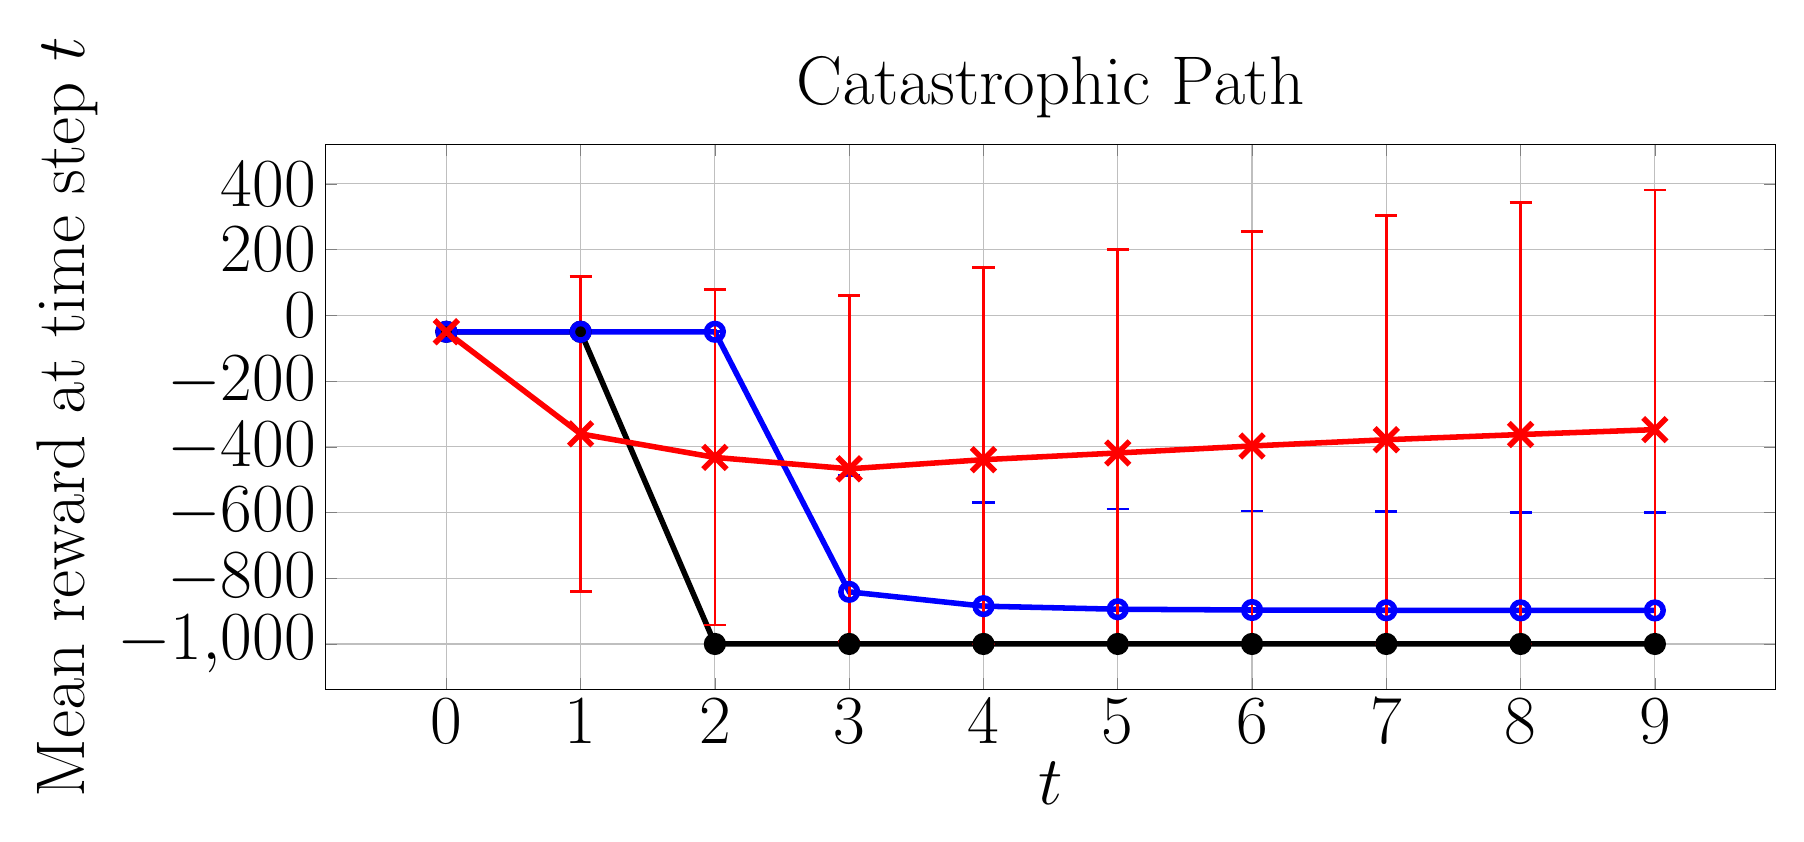
\begin{tikzpicture}
                \begin{axis}[
                    xlabel={$t$},
                    ylabel={Mean reward at time step $t$},
                    title={Catastrophic Path},
                    grid=both,
                    width=20cm, height=8.5cm,
                    every axis/.style={font=\Huge},
                    %
                ]
               \addplot[
                    color=black, %
                    mark=*, %
                    line width=2pt,
                    mark size=3pt,
                ]
                coordinates {
                    (0, -50.0)
                    (1, -50.0)
                    (2, -1000.0)
                    (3, -1000.0)
                    (4, -1000.0)
                    (5, -1000.0)
                    (6, -1000.0)
                    (7, -1000.0)
                    (8, -1000.0)
                    (9, -1000.0)
                };
                %
                %
                \addplot[
                    color=blue, %
                    mark=o, %
                    line width=2pt,
                    mark size=3pt,
                    error bars/.cd,
                    y dir=both, %
                    y explicit, %
                    error bar style={line width=1pt,solid},
                    error mark options={line width=1pt,mark size=4pt,rotate=90}
                ]
                coordinates {
                    (0, -50.0)  +- (0, 0.0)
                    (1, -50.0)  +- (0, 0.0) 
                    (2, -50.0)  +- (0, 0.0) 
                    (3, -841.440725)  += (0, 354.24605512) -= (0, 158.559275)
                    (4, -884.98225)  += (0, 315.37519669) -= (0, 115.01775)
                    (5, -894.330425) += (0, 304.88572805) -= (0, 105.669575)
                    (6, -896.696175) += (0, 301.19954514) -= (0, 103.303825)
                    (7, -897.4635) += (0, 299.61791279) -= (0, 102.5365)
                    (8, -897.77595) += (0, 298.80392585) -= (0, 102.22405)
                    (9, -897.942975) += (0, 298.32920557) -= (0, 102.057025)
                };
                %
                \addplot[
                    color=red, %
                    mark=x, %
                    line width=2pt,
                    mark size=6pt,
                    error bars/.cd,
                    y dir=both, %
                    y explicit, %
                    error bar style={line width=1pt,solid},
                    error mark options={line width=1pt,mark size=4pt,rotate=90}
                ]
            coordinates {
                    (0, -50.0)  +- (0, 0.0)
                    (1, -360.675265)  +- (0, 479.39812699) 
                    (2, -432.27629)  +- (0, 510.38620897) 
                    (3, -467.029545)  += (0, 526.36009628) -= (0, 526.36009628)
                    (4, -439.17429)  += (0, 583.96638919) -= (0, 560.82571)
                    (5, -418.82704) += (0, 618.43027478) -= (0, 581.17296)
                    (6, -397.464895) += (0, 652.67322574) -= (0, 602.535105)
                    (7, -378.49052) += (0, 682.85407033) -= (0, 621.50948)
                    (8, -362.654195) += (0, 707.01412023) -= (0, 637.345805)
                    (9, -347.737935) += (0, 729.29076479) -= (0, 652.262065)
                };
                %
                %
                %
                %
                %
                %
                %
                %
                %
                %
                %
                %
                %
                %
                %
                %
                %
                %
                %
                \end{axis}
            \end{tikzpicture}
         }
    }
    \caption{Average instant reward of CF paths induced by policies on Sepsis.}
    \label{fig: reward sepsis}
\end{figure*}

%
%
%
\subsection{Interval CFMDP Bounds}
%
%
Table \ref{tab:nonzero_probs} presents the mean counterfactual probability bound widths (excluding transitions where the upper bound is $0$) for each MDP, averaged over 20 observed paths. We compare the bounds under counterfactual stability (CS) and monotonicity (M) assumptions, CS alone, and no assumptions. This shows that the assumptions marginally reduce the bound widths, indicating the assumptions tighten the bounds without excluding too many causal models, as intended.
\renewcommand{\arraystretch}{1}

\begin{table}
\centering
\caption{Mean width of counterfactual probability bounds}
\resizebox{0.8\columnwidth}{!}{%
\begin{tabular}{|c|c|c|c|}
\hline
\multirow{2}{*}{\textbf{Environment}} & \multicolumn{3}{c|}{\textbf{Assumptions}} \\ \cline{2-4}
 & \textbf{CS + M} & \textbf{CS} & \textbf{None\tablefootnote{\jl{Equivalent to \citet{li2024probabilities}'s bounds (see Section \ref{sec: equivalence with Li}).}}} \\ \hline
\textbf{GridWorld} ($p=0.9$) & 0.0817 & 0.0977 & 0.100 \\ \hline
\textbf{GridWorld} ($p=0.4$) & 0.552  & 0.638  & 0.646 \\ \hline
\textbf{Sepsis} & 0.138 & 0.140 & 0.140 \\ \hline
\end{tabular}
}
\label{tab:nonzero_probs}
\end{table}


\subsection{Execution Times}
Table \ref{tab: times} compares the average time needed to generate the interval CFMDP vs.\ the Gumbel-max SCM CFMDP for 20 observations.
The GridWorld algorithms were run single-threaded, while the Sepsis experiments were run in parallel.
Generating the interval CFMDP is significantly faster as it uses exact analytical bounds, whereas the Gumbel-max CFMDP requires sampling from the Gumbel distribution to estimate counterfactual transition probabilities. \jl{Since constructing the counterfactual MDP models is the main bottleneck in both approaches, ours is more efficient overall and suitable for larger MDPs.}
\begin{table}
\centering
\caption{Mean execution time to generate CFMDPs}
\resizebox{0.99\columnwidth}{!}{%
\begin{tabular}{|c|c|c|}
\hline
\multirow{2}{*}{\textbf{Environment}} & \multicolumn{2}{c|}{\textbf{Mean Execution Time (s)}} \\ \cline{2-3} 
                                      & \textbf{Interval CFMDP} & \textbf{Gumbel-max CFMDP} \\ \hline
\textbf{GridWorld ($p=0.9$) }                  & 0.261                   & 56.1                      \\ \hline
\textbf{GridWorld ($p=0.4$)  }                 & 0.336                   & 54.5                      \\ \hline
\textbf{Sepsis}                                 & 688                     & 2940                      \\ \hline
\end{tabular}%
}
\label{tab: times}
\end{table}

%We present RiskHarvester, a risk-based tool to compute a security risk score based on the value of the asset and ease of attack on a database. We calculated the value of asset by identifying the sensitive data categories present in a database from the database keywords. We utilized data flow analysis, SQL, and Object Relational Mapper (ORM) parsing to identify the database keywords. To calculate the ease of attack, we utilized passive network analysis to retrieve the database host information. To evaluate RiskHarvester, we curated RiskBench, a benchmark of 1,791 database secret-asset pairs with sensitive data categories and host information manually retrieved from 188 GitHub repositories. RiskHarvester demonstrates precision of (95\%) and recall (90\%) in detecting database keywords for the value of asset and precision of (96\%) and recall (94\%) in detecting valid hosts for ease of attack. Finally, we conducted an online survey to understand whether developers prioritize secret removal based on security risk score. We found that 86\% of the developers prioritized the secrets for removal with descending security risk scores.

%%%%%%%%%%%%%%%%%%%%

\bibliographystyle{IEEEtran}
\bibliography{references}




%\subsection{Lloyd-Max Algorithm}
\label{subsec:Lloyd-Max}
For a given quantization bitwidth $B$ and an operand $\bm{X}$, the Lloyd-Max algorithm finds $2^B$ quantization levels $\{\hat{x}_i\}_{i=1}^{2^B}$ such that quantizing $\bm{X}$ by rounding each scalar in $\bm{X}$ to the nearest quantization level minimizes the quantization MSE. 

The algorithm starts with an initial guess of quantization levels and then iteratively computes quantization thresholds $\{\tau_i\}_{i=1}^{2^B-1}$ and updates quantization levels $\{\hat{x}_i\}_{i=1}^{2^B}$. Specifically, at iteration $n$, thresholds are set to the midpoints of the previous iteration's levels:
\begin{align*}
    \tau_i^{(n)}=\frac{\hat{x}_i^{(n-1)}+\hat{x}_{i+1}^{(n-1)}}2 \text{ for } i=1\ldots 2^B-1
\end{align*}
Subsequently, the quantization levels are re-computed as conditional means of the data regions defined by the new thresholds:
\begin{align*}
    \hat{x}_i^{(n)}=\mathbb{E}\left[ \bm{X} \big| \bm{X}\in [\tau_{i-1}^{(n)},\tau_i^{(n)}] \right] \text{ for } i=1\ldots 2^B
\end{align*}
where to satisfy boundary conditions we have $\tau_0=-\infty$ and $\tau_{2^B}=\infty$. The algorithm iterates the above steps until convergence.

Figure \ref{fig:lm_quant} compares the quantization levels of a $7$-bit floating point (E3M3) quantizer (left) to a $7$-bit Lloyd-Max quantizer (right) when quantizing a layer of weights from the GPT3-126M model at a per-tensor granularity. As shown, the Lloyd-Max quantizer achieves substantially lower quantization MSE. Further, Table \ref{tab:FP7_vs_LM7} shows the superior perplexity achieved by Lloyd-Max quantizers for bitwidths of $7$, $6$ and $5$. The difference between the quantizers is clear at 5 bits, where per-tensor FP quantization incurs a drastic and unacceptable increase in perplexity, while Lloyd-Max quantization incurs a much smaller increase. Nevertheless, we note that even the optimal Lloyd-Max quantizer incurs a notable ($\sim 1.5$) increase in perplexity due to the coarse granularity of quantization. 

\begin{figure}[h]
  \centering
  \includegraphics[width=0.7\linewidth]{sections/figures/LM7_FP7.pdf}
  \caption{\small Quantization levels and the corresponding quantization MSE of Floating Point (left) vs Lloyd-Max (right) Quantizers for a layer of weights in the GPT3-126M model.}
  \label{fig:lm_quant}
\end{figure}

\begin{table}[h]\scriptsize
\begin{center}
\caption{\label{tab:FP7_vs_LM7} \small Comparing perplexity (lower is better) achieved by floating point quantizers and Lloyd-Max quantizers on a GPT3-126M model for the Wikitext-103 dataset.}
\begin{tabular}{c|cc|c}
\hline
 \multirow{2}{*}{\textbf{Bitwidth}} & \multicolumn{2}{|c|}{\textbf{Floating-Point Quantizer}} & \textbf{Lloyd-Max Quantizer} \\
 & Best Format & Wikitext-103 Perplexity & Wikitext-103 Perplexity \\
\hline
7 & E3M3 & 18.32 & 18.27 \\
6 & E3M2 & 19.07 & 18.51 \\
5 & E4M0 & 43.89 & 19.71 \\
\hline
\end{tabular}
\end{center}
\end{table}

\subsection{Proof of Local Optimality of LO-BCQ}
\label{subsec:lobcq_opt_proof}
For a given block $\bm{b}_j$, the quantization MSE during LO-BCQ can be empirically evaluated as $\frac{1}{L_b}\lVert \bm{b}_j- \bm{\hat{b}}_j\rVert^2_2$ where $\bm{\hat{b}}_j$ is computed from equation (\ref{eq:clustered_quantization_definition}) as $C_{f(\bm{b}_j)}(\bm{b}_j)$. Further, for a given block cluster $\mathcal{B}_i$, we compute the quantization MSE as $\frac{1}{|\mathcal{B}_{i}|}\sum_{\bm{b} \in \mathcal{B}_{i}} \frac{1}{L_b}\lVert \bm{b}- C_i^{(n)}(\bm{b})\rVert^2_2$. Therefore, at the end of iteration $n$, we evaluate the overall quantization MSE $J^{(n)}$ for a given operand $\bm{X}$ composed of $N_c$ block clusters as:
\begin{align*}
    \label{eq:mse_iter_n}
    J^{(n)} = \frac{1}{N_c} \sum_{i=1}^{N_c} \frac{1}{|\mathcal{B}_{i}^{(n)}|}\sum_{\bm{v} \in \mathcal{B}_{i}^{(n)}} \frac{1}{L_b}\lVert \bm{b}- B_i^{(n)}(\bm{b})\rVert^2_2
\end{align*}

At the end of iteration $n$, the codebooks are updated from $\mathcal{C}^{(n-1)}$ to $\mathcal{C}^{(n)}$. However, the mapping of a given vector $\bm{b}_j$ to quantizers $\mathcal{C}^{(n)}$ remains as  $f^{(n)}(\bm{b}_j)$. At the next iteration, during the vector clustering step, $f^{(n+1)}(\bm{b}_j)$ finds new mapping of $\bm{b}_j$ to updated codebooks $\mathcal{C}^{(n)}$ such that the quantization MSE over the candidate codebooks is minimized. Therefore, we obtain the following result for $\bm{b}_j$:
\begin{align*}
\frac{1}{L_b}\lVert \bm{b}_j - C_{f^{(n+1)}(\bm{b}_j)}^{(n)}(\bm{b}_j)\rVert^2_2 \le \frac{1}{L_b}\lVert \bm{b}_j - C_{f^{(n)}(\bm{b}_j)}^{(n)}(\bm{b}_j)\rVert^2_2
\end{align*}

That is, quantizing $\bm{b}_j$ at the end of the block clustering step of iteration $n+1$ results in lower quantization MSE compared to quantizing at the end of iteration $n$. Since this is true for all $\bm{b} \in \bm{X}$, we assert the following:
\begin{equation}
\begin{split}
\label{eq:mse_ineq_1}
    \tilde{J}^{(n+1)} &= \frac{1}{N_c} \sum_{i=1}^{N_c} \frac{1}{|\mathcal{B}_{i}^{(n+1)}|}\sum_{\bm{b} \in \mathcal{B}_{i}^{(n+1)}} \frac{1}{L_b}\lVert \bm{b} - C_i^{(n)}(b)\rVert^2_2 \le J^{(n)}
\end{split}
\end{equation}
where $\tilde{J}^{(n+1)}$ is the the quantization MSE after the vector clustering step at iteration $n+1$.

Next, during the codebook update step (\ref{eq:quantizers_update}) at iteration $n+1$, the per-cluster codebooks $\mathcal{C}^{(n)}$ are updated to $\mathcal{C}^{(n+1)}$ by invoking the Lloyd-Max algorithm \citep{Lloyd}. We know that for any given value distribution, the Lloyd-Max algorithm minimizes the quantization MSE. Therefore, for a given vector cluster $\mathcal{B}_i$ we obtain the following result:

\begin{equation}
    \frac{1}{|\mathcal{B}_{i}^{(n+1)}|}\sum_{\bm{b} \in \mathcal{B}_{i}^{(n+1)}} \frac{1}{L_b}\lVert \bm{b}- C_i^{(n+1)}(\bm{b})\rVert^2_2 \le \frac{1}{|\mathcal{B}_{i}^{(n+1)}|}\sum_{\bm{b} \in \mathcal{B}_{i}^{(n+1)}} \frac{1}{L_b}\lVert \bm{b}- C_i^{(n)}(\bm{b})\rVert^2_2
\end{equation}

The above equation states that quantizing the given block cluster $\mathcal{B}_i$ after updating the associated codebook from $C_i^{(n)}$ to $C_i^{(n+1)}$ results in lower quantization MSE. Since this is true for all the block clusters, we derive the following result: 
\begin{equation}
\begin{split}
\label{eq:mse_ineq_2}
     J^{(n+1)} &= \frac{1}{N_c} \sum_{i=1}^{N_c} \frac{1}{|\mathcal{B}_{i}^{(n+1)}|}\sum_{\bm{b} \in \mathcal{B}_{i}^{(n+1)}} \frac{1}{L_b}\lVert \bm{b}- C_i^{(n+1)}(\bm{b})\rVert^2_2  \le \tilde{J}^{(n+1)}   
\end{split}
\end{equation}

Following (\ref{eq:mse_ineq_1}) and (\ref{eq:mse_ineq_2}), we find that the quantization MSE is non-increasing for each iteration, that is, $J^{(1)} \ge J^{(2)} \ge J^{(3)} \ge \ldots \ge J^{(M)}$ where $M$ is the maximum number of iterations. 
%Therefore, we can say that if the algorithm converges, then it must be that it has converged to a local minimum. 
\hfill $\blacksquare$


\begin{figure}
    \begin{center}
    \includegraphics[width=0.5\textwidth]{sections//figures/mse_vs_iter.pdf}
    \end{center}
    \caption{\small NMSE vs iterations during LO-BCQ compared to other block quantization proposals}
    \label{fig:nmse_vs_iter}
\end{figure}

Figure \ref{fig:nmse_vs_iter} shows the empirical convergence of LO-BCQ across several block lengths and number of codebooks. Also, the MSE achieved by LO-BCQ is compared to baselines such as MXFP and VSQ. As shown, LO-BCQ converges to a lower MSE than the baselines. Further, we achieve better convergence for larger number of codebooks ($N_c$) and for a smaller block length ($L_b$), both of which increase the bitwidth of BCQ (see Eq \ref{eq:bitwidth_bcq}).


\subsection{Additional Accuracy Results}
%Table \ref{tab:lobcq_config} lists the various LOBCQ configurations and their corresponding bitwidths.
\begin{table}
\setlength{\tabcolsep}{4.75pt}
\begin{center}
\caption{\label{tab:lobcq_config} Various LO-BCQ configurations and their bitwidths.}
\begin{tabular}{|c||c|c|c|c||c|c||c|} 
\hline
 & \multicolumn{4}{|c||}{$L_b=8$} & \multicolumn{2}{|c||}{$L_b=4$} & $L_b=2$ \\
 \hline
 \backslashbox{$L_A$\kern-1em}{\kern-1em$N_c$} & 2 & 4 & 8 & 16 & 2 & 4 & 2 \\
 \hline
 64 & 4.25 & 4.375 & 4.5 & 4.625 & 4.375 & 4.625 & 4.625\\
 \hline
 32 & 4.375 & 4.5 & 4.625& 4.75 & 4.5 & 4.75 & 4.75 \\
 \hline
 16 & 4.625 & 4.75& 4.875 & 5 & 4.75 & 5 & 5 \\
 \hline
\end{tabular}
\end{center}
\end{table}

%\subsection{Perplexity achieved by various LO-BCQ configurations on Wikitext-103 dataset}

\begin{table} \centering
\begin{tabular}{|c||c|c|c|c||c|c||c|} 
\hline
 $L_b \rightarrow$& \multicolumn{4}{c||}{8} & \multicolumn{2}{c||}{4} & 2\\
 \hline
 \backslashbox{$L_A$\kern-1em}{\kern-1em$N_c$} & 2 & 4 & 8 & 16 & 2 & 4 & 2  \\
 %$N_c \rightarrow$ & 2 & 4 & 8 & 16 & 2 & 4 & 2 \\
 \hline
 \hline
 \multicolumn{8}{c}{GPT3-1.3B (FP32 PPL = 9.98)} \\ 
 \hline
 \hline
 64 & 10.40 & 10.23 & 10.17 & 10.15 &  10.28 & 10.18 & 10.19 \\
 \hline
 32 & 10.25 & 10.20 & 10.15 & 10.12 &  10.23 & 10.17 & 10.17 \\
 \hline
 16 & 10.22 & 10.16 & 10.10 & 10.09 &  10.21 & 10.14 & 10.16 \\
 \hline
  \hline
 \multicolumn{8}{c}{GPT3-8B (FP32 PPL = 7.38)} \\ 
 \hline
 \hline
 64 & 7.61 & 7.52 & 7.48 &  7.47 &  7.55 &  7.49 & 7.50 \\
 \hline
 32 & 7.52 & 7.50 & 7.46 &  7.45 &  7.52 &  7.48 & 7.48  \\
 \hline
 16 & 7.51 & 7.48 & 7.44 &  7.44 &  7.51 &  7.49 & 7.47  \\
 \hline
\end{tabular}
\caption{\label{tab:ppl_gpt3_abalation} Wikitext-103 perplexity across GPT3-1.3B and 8B models.}
\end{table}

\begin{table} \centering
\begin{tabular}{|c||c|c|c|c||} 
\hline
 $L_b \rightarrow$& \multicolumn{4}{c||}{8}\\
 \hline
 \backslashbox{$L_A$\kern-1em}{\kern-1em$N_c$} & 2 & 4 & 8 & 16 \\
 %$N_c \rightarrow$ & 2 & 4 & 8 & 16 & 2 & 4 & 2 \\
 \hline
 \hline
 \multicolumn{5}{|c|}{Llama2-7B (FP32 PPL = 5.06)} \\ 
 \hline
 \hline
 64 & 5.31 & 5.26 & 5.19 & 5.18  \\
 \hline
 32 & 5.23 & 5.25 & 5.18 & 5.15  \\
 \hline
 16 & 5.23 & 5.19 & 5.16 & 5.14  \\
 \hline
 \multicolumn{5}{|c|}{Nemotron4-15B (FP32 PPL = 5.87)} \\ 
 \hline
 \hline
 64  & 6.3 & 6.20 & 6.13 & 6.08  \\
 \hline
 32  & 6.24 & 6.12 & 6.07 & 6.03  \\
 \hline
 16  & 6.12 & 6.14 & 6.04 & 6.02  \\
 \hline
 \multicolumn{5}{|c|}{Nemotron4-340B (FP32 PPL = 3.48)} \\ 
 \hline
 \hline
 64 & 3.67 & 3.62 & 3.60 & 3.59 \\
 \hline
 32 & 3.63 & 3.61 & 3.59 & 3.56 \\
 \hline
 16 & 3.61 & 3.58 & 3.57 & 3.55 \\
 \hline
\end{tabular}
\caption{\label{tab:ppl_llama7B_nemo15B} Wikitext-103 perplexity compared to FP32 baseline in Llama2-7B and Nemotron4-15B, 340B models}
\end{table}

%\subsection{Perplexity achieved by various LO-BCQ configurations on MMLU dataset}


\begin{table} \centering
\begin{tabular}{|c||c|c|c|c||c|c|c|c|} 
\hline
 $L_b \rightarrow$& \multicolumn{4}{c||}{8} & \multicolumn{4}{c||}{8}\\
 \hline
 \backslashbox{$L_A$\kern-1em}{\kern-1em$N_c$} & 2 & 4 & 8 & 16 & 2 & 4 & 8 & 16  \\
 %$N_c \rightarrow$ & 2 & 4 & 8 & 16 & 2 & 4 & 2 \\
 \hline
 \hline
 \multicolumn{5}{|c|}{Llama2-7B (FP32 Accuracy = 45.8\%)} & \multicolumn{4}{|c|}{Llama2-70B (FP32 Accuracy = 69.12\%)} \\ 
 \hline
 \hline
 64 & 43.9 & 43.4 & 43.9 & 44.9 & 68.07 & 68.27 & 68.17 & 68.75 \\
 \hline
 32 & 44.5 & 43.8 & 44.9 & 44.5 & 68.37 & 68.51 & 68.35 & 68.27  \\
 \hline
 16 & 43.9 & 42.7 & 44.9 & 45 & 68.12 & 68.77 & 68.31 & 68.59  \\
 \hline
 \hline
 \multicolumn{5}{|c|}{GPT3-22B (FP32 Accuracy = 38.75\%)} & \multicolumn{4}{|c|}{Nemotron4-15B (FP32 Accuracy = 64.3\%)} \\ 
 \hline
 \hline
 64 & 36.71 & 38.85 & 38.13 & 38.92 & 63.17 & 62.36 & 63.72 & 64.09 \\
 \hline
 32 & 37.95 & 38.69 & 39.45 & 38.34 & 64.05 & 62.30 & 63.8 & 64.33  \\
 \hline
 16 & 38.88 & 38.80 & 38.31 & 38.92 & 63.22 & 63.51 & 63.93 & 64.43  \\
 \hline
\end{tabular}
\caption{\label{tab:mmlu_abalation} Accuracy on MMLU dataset across GPT3-22B, Llama2-7B, 70B and Nemotron4-15B models.}
\end{table}


%\subsection{Perplexity achieved by various LO-BCQ configurations on LM evaluation harness}

\begin{table} \centering
\begin{tabular}{|c||c|c|c|c||c|c|c|c|} 
\hline
 $L_b \rightarrow$& \multicolumn{4}{c||}{8} & \multicolumn{4}{c||}{8}\\
 \hline
 \backslashbox{$L_A$\kern-1em}{\kern-1em$N_c$} & 2 & 4 & 8 & 16 & 2 & 4 & 8 & 16  \\
 %$N_c \rightarrow$ & 2 & 4 & 8 & 16 & 2 & 4 & 2 \\
 \hline
 \hline
 \multicolumn{5}{|c|}{Race (FP32 Accuracy = 37.51\%)} & \multicolumn{4}{|c|}{Boolq (FP32 Accuracy = 64.62\%)} \\ 
 \hline
 \hline
 64 & 36.94 & 37.13 & 36.27 & 37.13 & 63.73 & 62.26 & 63.49 & 63.36 \\
 \hline
 32 & 37.03 & 36.36 & 36.08 & 37.03 & 62.54 & 63.51 & 63.49 & 63.55  \\
 \hline
 16 & 37.03 & 37.03 & 36.46 & 37.03 & 61.1 & 63.79 & 63.58 & 63.33  \\
 \hline
 \hline
 \multicolumn{5}{|c|}{Winogrande (FP32 Accuracy = 58.01\%)} & \multicolumn{4}{|c|}{Piqa (FP32 Accuracy = 74.21\%)} \\ 
 \hline
 \hline
 64 & 58.17 & 57.22 & 57.85 & 58.33 & 73.01 & 73.07 & 73.07 & 72.80 \\
 \hline
 32 & 59.12 & 58.09 & 57.85 & 58.41 & 73.01 & 73.94 & 72.74 & 73.18  \\
 \hline
 16 & 57.93 & 58.88 & 57.93 & 58.56 & 73.94 & 72.80 & 73.01 & 73.94  \\
 \hline
\end{tabular}
\caption{\label{tab:mmlu_abalation} Accuracy on LM evaluation harness tasks on GPT3-1.3B model.}
\end{table}

\begin{table} \centering
\begin{tabular}{|c||c|c|c|c||c|c|c|c|} 
\hline
 $L_b \rightarrow$& \multicolumn{4}{c||}{8} & \multicolumn{4}{c||}{8}\\
 \hline
 \backslashbox{$L_A$\kern-1em}{\kern-1em$N_c$} & 2 & 4 & 8 & 16 & 2 & 4 & 8 & 16  \\
 %$N_c \rightarrow$ & 2 & 4 & 8 & 16 & 2 & 4 & 2 \\
 \hline
 \hline
 \multicolumn{5}{|c|}{Race (FP32 Accuracy = 41.34\%)} & \multicolumn{4}{|c|}{Boolq (FP32 Accuracy = 68.32\%)} \\ 
 \hline
 \hline
 64 & 40.48 & 40.10 & 39.43 & 39.90 & 69.20 & 68.41 & 69.45 & 68.56 \\
 \hline
 32 & 39.52 & 39.52 & 40.77 & 39.62 & 68.32 & 67.43 & 68.17 & 69.30  \\
 \hline
 16 & 39.81 & 39.71 & 39.90 & 40.38 & 68.10 & 66.33 & 69.51 & 69.42  \\
 \hline
 \hline
 \multicolumn{5}{|c|}{Winogrande (FP32 Accuracy = 67.88\%)} & \multicolumn{4}{|c|}{Piqa (FP32 Accuracy = 78.78\%)} \\ 
 \hline
 \hline
 64 & 66.85 & 66.61 & 67.72 & 67.88 & 77.31 & 77.42 & 77.75 & 77.64 \\
 \hline
 32 & 67.25 & 67.72 & 67.72 & 67.00 & 77.31 & 77.04 & 77.80 & 77.37  \\
 \hline
 16 & 68.11 & 68.90 & 67.88 & 67.48 & 77.37 & 78.13 & 78.13 & 77.69  \\
 \hline
\end{tabular}
\caption{\label{tab:mmlu_abalation} Accuracy on LM evaluation harness tasks on GPT3-8B model.}
\end{table}

\begin{table} \centering
\begin{tabular}{|c||c|c|c|c||c|c|c|c|} 
\hline
 $L_b \rightarrow$& \multicolumn{4}{c||}{8} & \multicolumn{4}{c||}{8}\\
 \hline
 \backslashbox{$L_A$\kern-1em}{\kern-1em$N_c$} & 2 & 4 & 8 & 16 & 2 & 4 & 8 & 16  \\
 %$N_c \rightarrow$ & 2 & 4 & 8 & 16 & 2 & 4 & 2 \\
 \hline
 \hline
 \multicolumn{5}{|c|}{Race (FP32 Accuracy = 40.67\%)} & \multicolumn{4}{|c|}{Boolq (FP32 Accuracy = 76.54\%)} \\ 
 \hline
 \hline
 64 & 40.48 & 40.10 & 39.43 & 39.90 & 75.41 & 75.11 & 77.09 & 75.66 \\
 \hline
 32 & 39.52 & 39.52 & 40.77 & 39.62 & 76.02 & 76.02 & 75.96 & 75.35  \\
 \hline
 16 & 39.81 & 39.71 & 39.90 & 40.38 & 75.05 & 73.82 & 75.72 & 76.09  \\
 \hline
 \hline
 \multicolumn{5}{|c|}{Winogrande (FP32 Accuracy = 70.64\%)} & \multicolumn{4}{|c|}{Piqa (FP32 Accuracy = 79.16\%)} \\ 
 \hline
 \hline
 64 & 69.14 & 70.17 & 70.17 & 70.56 & 78.24 & 79.00 & 78.62 & 78.73 \\
 \hline
 32 & 70.96 & 69.69 & 71.27 & 69.30 & 78.56 & 79.49 & 79.16 & 78.89  \\
 \hline
 16 & 71.03 & 69.53 & 69.69 & 70.40 & 78.13 & 79.16 & 79.00 & 79.00  \\
 \hline
\end{tabular}
\caption{\label{tab:mmlu_abalation} Accuracy on LM evaluation harness tasks on GPT3-22B model.}
\end{table}

\begin{table} \centering
\begin{tabular}{|c||c|c|c|c||c|c|c|c|} 
\hline
 $L_b \rightarrow$& \multicolumn{4}{c||}{8} & \multicolumn{4}{c||}{8}\\
 \hline
 \backslashbox{$L_A$\kern-1em}{\kern-1em$N_c$} & 2 & 4 & 8 & 16 & 2 & 4 & 8 & 16  \\
 %$N_c \rightarrow$ & 2 & 4 & 8 & 16 & 2 & 4 & 2 \\
 \hline
 \hline
 \multicolumn{5}{|c|}{Race (FP32 Accuracy = 44.4\%)} & \multicolumn{4}{|c|}{Boolq (FP32 Accuracy = 79.29\%)} \\ 
 \hline
 \hline
 64 & 42.49 & 42.51 & 42.58 & 43.45 & 77.58 & 77.37 & 77.43 & 78.1 \\
 \hline
 32 & 43.35 & 42.49 & 43.64 & 43.73 & 77.86 & 75.32 & 77.28 & 77.86  \\
 \hline
 16 & 44.21 & 44.21 & 43.64 & 42.97 & 78.65 & 77 & 76.94 & 77.98  \\
 \hline
 \hline
 \multicolumn{5}{|c|}{Winogrande (FP32 Accuracy = 69.38\%)} & \multicolumn{4}{|c|}{Piqa (FP32 Accuracy = 78.07\%)} \\ 
 \hline
 \hline
 64 & 68.9 & 68.43 & 69.77 & 68.19 & 77.09 & 76.82 & 77.09 & 77.86 \\
 \hline
 32 & 69.38 & 68.51 & 68.82 & 68.90 & 78.07 & 76.71 & 78.07 & 77.86  \\
 \hline
 16 & 69.53 & 67.09 & 69.38 & 68.90 & 77.37 & 77.8 & 77.91 & 77.69  \\
 \hline
\end{tabular}
\caption{\label{tab:mmlu_abalation} Accuracy on LM evaluation harness tasks on Llama2-7B model.}
\end{table}

\begin{table} \centering
\begin{tabular}{|c||c|c|c|c||c|c|c|c|} 
\hline
 $L_b \rightarrow$& \multicolumn{4}{c||}{8} & \multicolumn{4}{c||}{8}\\
 \hline
 \backslashbox{$L_A$\kern-1em}{\kern-1em$N_c$} & 2 & 4 & 8 & 16 & 2 & 4 & 8 & 16  \\
 %$N_c \rightarrow$ & 2 & 4 & 8 & 16 & 2 & 4 & 2 \\
 \hline
 \hline
 \multicolumn{5}{|c|}{Race (FP32 Accuracy = 48.8\%)} & \multicolumn{4}{|c|}{Boolq (FP32 Accuracy = 85.23\%)} \\ 
 \hline
 \hline
 64 & 49.00 & 49.00 & 49.28 & 48.71 & 82.82 & 84.28 & 84.03 & 84.25 \\
 \hline
 32 & 49.57 & 48.52 & 48.33 & 49.28 & 83.85 & 84.46 & 84.31 & 84.93  \\
 \hline
 16 & 49.85 & 49.09 & 49.28 & 48.99 & 85.11 & 84.46 & 84.61 & 83.94  \\
 \hline
 \hline
 \multicolumn{5}{|c|}{Winogrande (FP32 Accuracy = 79.95\%)} & \multicolumn{4}{|c|}{Piqa (FP32 Accuracy = 81.56\%)} \\ 
 \hline
 \hline
 64 & 78.77 & 78.45 & 78.37 & 79.16 & 81.45 & 80.69 & 81.45 & 81.5 \\
 \hline
 32 & 78.45 & 79.01 & 78.69 & 80.66 & 81.56 & 80.58 & 81.18 & 81.34  \\
 \hline
 16 & 79.95 & 79.56 & 79.79 & 79.72 & 81.28 & 81.66 & 81.28 & 80.96  \\
 \hline
\end{tabular}
\caption{\label{tab:mmlu_abalation} Accuracy on LM evaluation harness tasks on Llama2-70B model.}
\end{table}

%\section{MSE Studies}
%\textcolor{red}{TODO}


\subsection{Number Formats and Quantization Method}
\label{subsec:numFormats_quantMethod}
\subsubsection{Integer Format}
An $n$-bit signed integer (INT) is typically represented with a 2s-complement format \citep{yao2022zeroquant,xiao2023smoothquant,dai2021vsq}, where the most significant bit denotes the sign.

\subsubsection{Floating Point Format}
An $n$-bit signed floating point (FP) number $x$ comprises of a 1-bit sign ($x_{\mathrm{sign}}$), $B_m$-bit mantissa ($x_{\mathrm{mant}}$) and $B_e$-bit exponent ($x_{\mathrm{exp}}$) such that $B_m+B_e=n-1$. The associated constant exponent bias ($E_{\mathrm{bias}}$) is computed as $(2^{{B_e}-1}-1)$. We denote this format as $E_{B_e}M_{B_m}$.  

\subsubsection{Quantization Scheme}
\label{subsec:quant_method}
A quantization scheme dictates how a given unquantized tensor is converted to its quantized representation. We consider FP formats for the purpose of illustration. Given an unquantized tensor $\bm{X}$ and an FP format $E_{B_e}M_{B_m}$, we first, we compute the quantization scale factor $s_X$ that maps the maximum absolute value of $\bm{X}$ to the maximum quantization level of the $E_{B_e}M_{B_m}$ format as follows:
\begin{align}
\label{eq:sf}
    s_X = \frac{\mathrm{max}(|\bm{X}|)}{\mathrm{max}(E_{B_e}M_{B_m})}
\end{align}
In the above equation, $|\cdot|$ denotes the absolute value function.

Next, we scale $\bm{X}$ by $s_X$ and quantize it to $\hat{\bm{X}}$ by rounding it to the nearest quantization level of $E_{B_e}M_{B_m}$ as:

\begin{align}
\label{eq:tensor_quant}
    \hat{\bm{X}} = \text{round-to-nearest}\left(\frac{\bm{X}}{s_X}, E_{B_e}M_{B_m}\right)
\end{align}

We perform dynamic max-scaled quantization \citep{wu2020integer}, where the scale factor $s$ for activations is dynamically computed during runtime.

\subsection{Vector Scaled Quantization}
\begin{wrapfigure}{r}{0.35\linewidth}
  \centering
  \includegraphics[width=\linewidth]{sections/figures/vsquant.jpg}
  \caption{\small Vectorwise decomposition for per-vector scaled quantization (VSQ \citep{dai2021vsq}).}
  \label{fig:vsquant}
\end{wrapfigure}
During VSQ \citep{dai2021vsq}, the operand tensors are decomposed into 1D vectors in a hardware friendly manner as shown in Figure \ref{fig:vsquant}. Since the decomposed tensors are used as operands in matrix multiplications during inference, it is beneficial to perform this decomposition along the reduction dimension of the multiplication. The vectorwise quantization is performed similar to tensorwise quantization described in Equations \ref{eq:sf} and \ref{eq:tensor_quant}, where a scale factor $s_v$ is required for each vector $\bm{v}$ that maps the maximum absolute value of that vector to the maximum quantization level. While smaller vector lengths can lead to larger accuracy gains, the associated memory and computational overheads due to the per-vector scale factors increases. To alleviate these overheads, VSQ \citep{dai2021vsq} proposed a second level quantization of the per-vector scale factors to unsigned integers, while MX \citep{rouhani2023shared} quantizes them to integer powers of 2 (denoted as $2^{INT}$).

\subsubsection{MX Format}
The MX format proposed in \citep{rouhani2023microscaling} introduces the concept of sub-block shifting. For every two scalar elements of $b$-bits each, there is a shared exponent bit. The value of this exponent bit is determined through an empirical analysis that targets minimizing quantization MSE. We note that the FP format $E_{1}M_{b}$ is strictly better than MX from an accuracy perspective since it allocates a dedicated exponent bit to each scalar as opposed to sharing it across two scalars. Therefore, we conservatively bound the accuracy of a $b+2$-bit signed MX format with that of a $E_{1}M_{b}$ format in our comparisons. For instance, we use E1M2 format as a proxy for MX4.

\begin{figure}
    \centering
    \includegraphics[width=1\linewidth]{sections//figures/BlockFormats.pdf}
    \caption{\small Comparing LO-BCQ to MX format.}
    \label{fig:block_formats}
\end{figure}

Figure \ref{fig:block_formats} compares our $4$-bit LO-BCQ block format to MX \citep{rouhani2023microscaling}. As shown, both LO-BCQ and MX decompose a given operand tensor into block arrays and each block array into blocks. Similar to MX, we find that per-block quantization ($L_b < L_A$) leads to better accuracy due to increased flexibility. While MX achieves this through per-block $1$-bit micro-scales, we associate a dedicated codebook to each block through a per-block codebook selector. Further, MX quantizes the per-block array scale-factor to E8M0 format without per-tensor scaling. In contrast during LO-BCQ, we find that per-tensor scaling combined with quantization of per-block array scale-factor to E4M3 format results in superior inference accuracy across models. 


\end{document}

%%%%%%%%%%%%%%%%%%%%%%%%%%%%%%%%%%%%%%%%%

